\chapter{Linearization Results}
\label{LinResults}
\subsection{Estimation Data}

As the parameter estimation is based on a linearized model an operating point for the system is chosen. This point is based on the tank level being approximately half way full which allows for an equal amount of deviation in both directions. For the chosen operating point, data is gather from the system while small steps are individually applied to the two main pumps and the opening degree of the PMA valves. In order to use the data for parameter estimation the operating point is subtracted, leaving only small signal values.  

The operating point of the PMA valves is chosen to $63^{\circ}$ and the small signal values for the estimation can be seen in \figref{fig:est_OD_data}.

\begin{figure}[H]
\centering
% This file was created by matlab2tikz.
%
%The latest updates can be retrieved from
%  http://www.mathworks.com/matlabcentral/fileexchange/22022-matlab2tikz-matlab2tikz
%where you can also make suggestions and rate matlab2tikz.
%
\definecolor{mycolor1}{rgb}{0.00000,0.44700,0.74100}%
\definecolor{mycolor2}{rgb}{0.85000,0.32500,0.09800}%
\definecolor{mycolor3}{rgb}{0.92900,0.69400,0.12500}%
\definecolor{mycolor4}{rgb}{0.49400,0.18400,0.55600}%
%
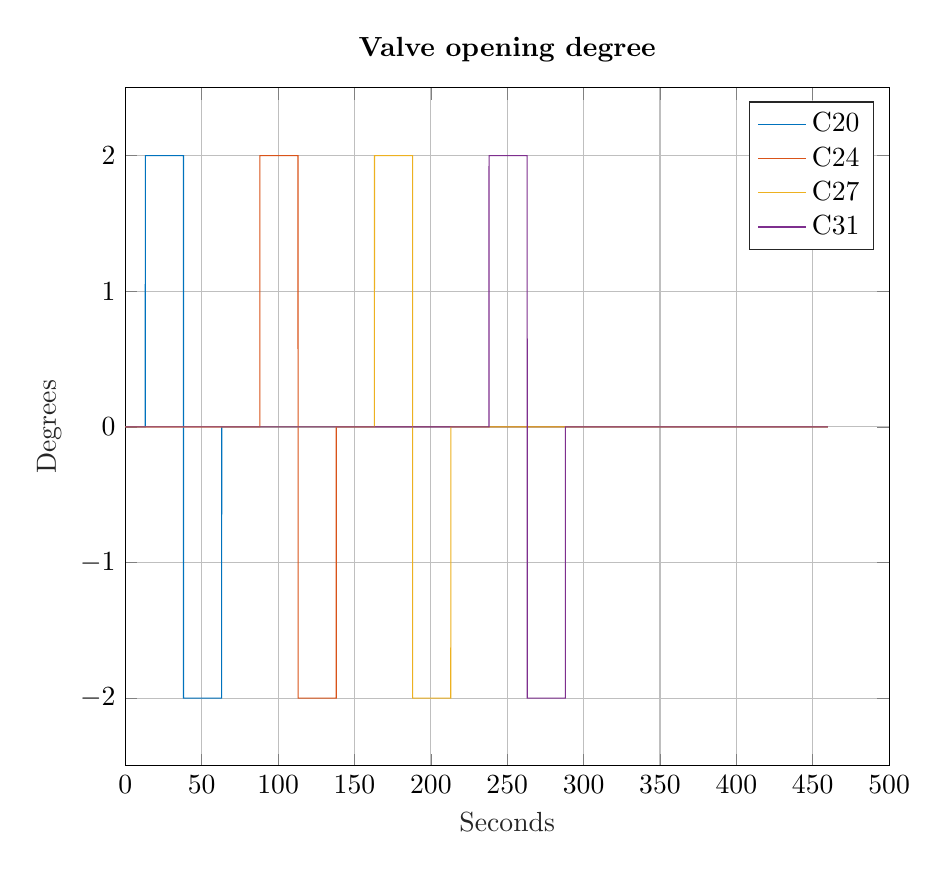
\begin{tikzpicture}

\begin{axis}[%
width=0.8\textwidth,
height=3.39in,
at={(0.758in,0.481in)},
scale only axis,
xmin=0,
xmax=500,
xlabel style={font=\color{white!15!black}},
xlabel={Seconds},
ymin=-2.5,
ymax=2.5,
ylabel style={font=\color{white!15!black}},
ylabel={Degrees},
axis background/.style={fill=white},
title style={font=\bfseries},
title={Valve opening degree},
xmajorgrids,
ymajorgrids,
legend style={legend cell align=left, align=left, draw=white!15!black}
]
\addplot [color=mycolor1]
  table[row sep=crcr]{%
0	-1.13686837721616e-13\\
13.05	-1.13686837721616e-13\\
13.1	1.99999999999989\\
38.05	1.99999999999989\\
38.1	-2.00000000000006\\
63.05	-2.00000000000006\\
63.1	-1.13686837721616e-13\\
459.95	-1.13686837721616e-13\\
};
\addlegendentry{C20}

\addplot [color=mycolor2]
  table[row sep=crcr]{%
0	-1.13686837721616e-13\\
88.05	-1.13686837721616e-13\\
88.1	1.99999999999989\\
113.05	1.99999999999989\\
113.1	-2.00000000000006\\
138.05	-2.00000000000006\\
138.1	-1.13686837721616e-13\\
459.95	-1.13686837721616e-13\\
};
\addlegendentry{C24}

\addplot [color=mycolor3]
  table[row sep=crcr]{%
0	-1.13686837721616e-13\\
163.05	-1.13686837721616e-13\\
163.1	1.99999999999989\\
188.05	1.99999999999989\\
188.1	-2.00000000000006\\
213.05	-2.00000000000006\\
213.1	-1.13686837721616e-13\\
459.95	-1.13686837721616e-13\\
};
\addlegendentry{C27}

\addplot [color=mycolor4]
  table[row sep=crcr]{%
0	-1.13686837721616e-13\\
238.05	-1.13686837721616e-13\\
238.1	1.99999999999989\\
263.05	1.99999999999989\\
263.1	-2.00000000000006\\
288.05	-2.00000000000006\\
288.1	-1.13686837721616e-13\\
459.95	-1.13686837721616e-13\\
};
\addlegendentry{C31}

\end{axis}
\end{tikzpicture}% 
\caption{Small signal values of the opening degrees of the pma valves. }
\label{fig:est_OD_data}
\end{figure}

Furthermore the operating point for the pumps is chosen at a speed of $\omega = 0.4$, where the small signal values for the estimation are shown in \figref{fig:est_deltap_data}. 

\begin{figure}[H]
\centering
% This file was created by matlab2tikz.
%
%The latest updates can be retrieved from
%  http://www.mathworks.com/matlabcentral/fileexchange/22022-matlab2tikz-matlab2tikz
%where you can also make suggestions and rate matlab2tikz.
%
\definecolor{mycolor1}{rgb}{0.00000,0.44700,0.74100}%
\definecolor{mycolor2}{rgb}{0.85000,0.32500,0.09800}%
%
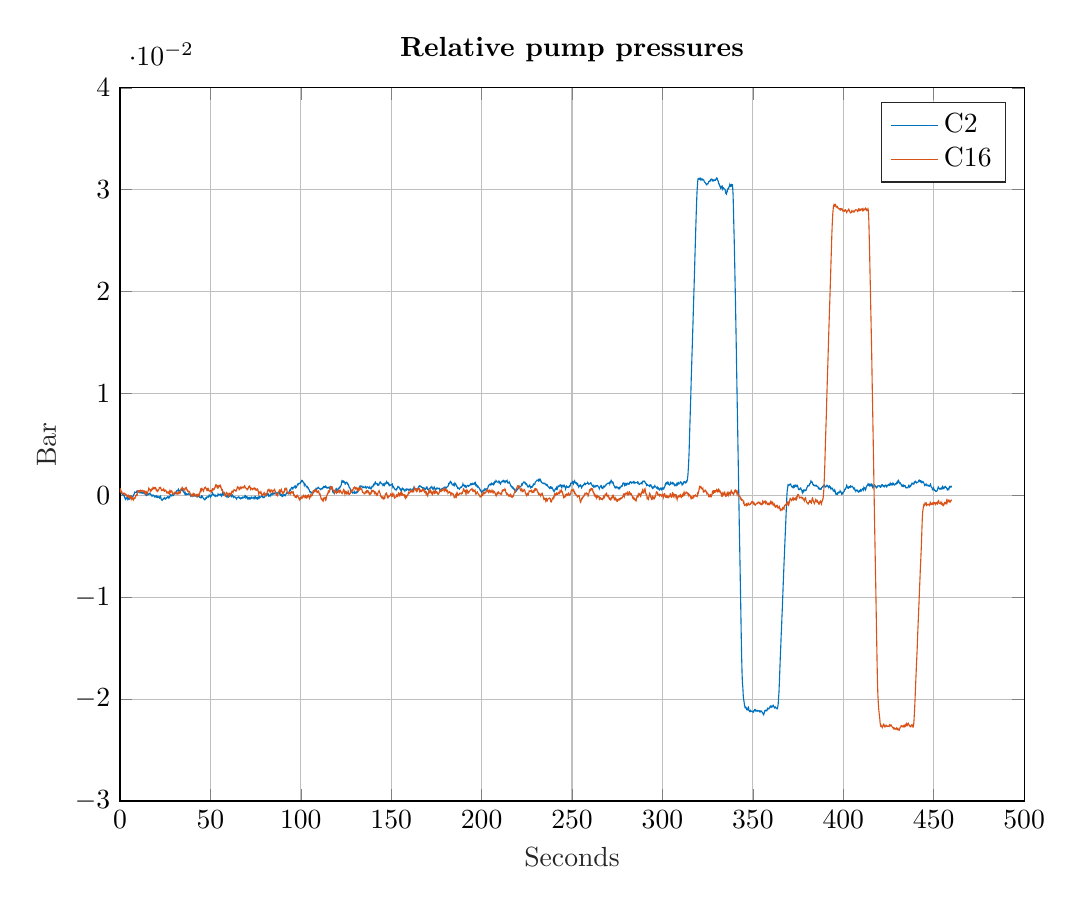
\begin{tikzpicture}

\begin{axis}[%
width=4.521in,
height=3.566in,
at={(0.758in,0.481in)},
scale only axis,
xmin=0,
xmax=500,
xlabel style={font=\color{white!15!black}},
xlabel={Seconds},
ymin=-0.03,
ymax=0.04,
ylabel style={font=\color{white!15!black}},
ylabel={Bar},
axis background/.style={fill=white},
title style={font=\bfseries},
title={Relative pump pressures},
xmajorgrids,
ymajorgrids,
legend style={legend cell align=left, align=left, draw=white!15!black}
]
\addplot [color=mycolor1]
  table[row sep=crcr]{%
0	0.000522666177914743\\
0.100000000000023	0.000486009286419176\\
0.300000000000011	0.000443242912979258\\
0.399999999999977	0.000394367057651834\\
0.5	0.000369929129988122\\
0.649999999999977	0.000235520527837707\\
0.899999999999977	0.000223301564005851\\
1.19999999999999	0.000125549853351004\\
1.44999999999999	0.000174425708678427\\
1.89999999999998	4.00171065280119e-05\\
2	-1.49682306869181e-05\\
2.25	-3.940615835063e-05\\
2.44999999999999	-7.60630498461978e-05\\
2.69999999999999	-0.000234909579660325\\
2.80000000000001	-0.000216581133940963\\
2.94999999999999	-0.000259347507324037\\
3.10000000000002	-0.000424303519082514\\
3.14999999999998	-0.000424303519082514\\
3.25	-0.00037542766375509\\
3.85000000000002	-0.000210471651996613\\
3.89999999999998	-0.000167705278613539\\
4.05000000000001	-0.000137157869005478\\
4.14999999999998	-0.000234909579660325\\
4.30000000000001	-0.000344880254147029\\
4.44999999999999	-0.000241019061604675\\
4.94999999999999	-0.000369318181810741\\
5.10000000000002	-0.00031433284459581\\
5.19999999999999	-0.000357099217978885\\
5.30000000000001	-0.000338770772259522\\
5.55000000000001	-0.000271566471155893\\
5.60000000000002	-0.000228800097772819\\
5.69999999999999	-0.000222690615828469\\
5.80000000000001	-0.000204362170109107\\
5.89999999999998	-0.000192143206277251\\
6	-0.000198252688164757\\
6.19999999999999	-0.000149376832837334\\
6.35000000000002	-0.000228800097772819\\
6.44999999999999	-0.000265456989268387\\
6.5	-0.000259347507324037\\
6.64999999999998	-0.000167705278613539\\
7	-0.000143267350949827\\
7.14999999999998	-0.000149376832837334\\
7.35000000000002	-2.7187194518774e-05\\
7.44999999999999	-2.74926685506216e-06\\
7.55000000000001	4.61265884723616e-05\\
7.64999999999998	6.44550341917238e-05\\
7.69999999999999	0.000101111925687292\\
7.89999999999998	0.000143878299127209\\
8.05000000000001	0.000272177419333275\\
8.10000000000002	0.000327162756605048\\
8.19999999999999	0.000339381720436904\\
8.30000000000001	0.000333272238492555\\
9	0.000272177419333275\\
9.30000000000001	0.000394367057651834\\
9.39999999999998	0.000345491202324411\\
9.5	0.00035160068426876\\
9.75	0.000431023949147402\\
10.35	0.000418804985315546\\
10.45	0.000388257575764328\\
10.75	0.000437133431091752\\
11.1	0.000247739491669563\\
11.4	0.000308834310828843\\
11.55	0.000321053274660699\\
11.65	0.000308834310828843\\
11.75	0.000302724828941336\\
11.85	0.000241630009782057\\
11.95	0.000235520527837707\\
12.05	0.000278286901277625\\
12.25	0.000259958455501419\\
12.4	0.000217192082118345\\
12.55	0.000235520527837707\\
12.65	0.000278286901277625\\
12.75	0.000284396383165131\\
12.9	0.000290505865109481\\
13	0.000290505865109481\\
13.1	0.000296615346996987\\
13.25	0.000186644672510283\\
13.45	0.000192754154454633\\
13.5	0.000217192082118345\\
14.1	8.88929618554357e-05\\
14.3	0.000137768817182859\\
14.65	-1.49682306869181e-05\\
14.9	3.3602150324441e-06\\
14.95	2.16886608086497e-05\\
15.05	0.000101111925687292\\
15.2	0.000137768817182859\\
15.35	0.000107221407631641\\
15.5	0.000131659335295353\\
15.7	8.27834799679295e-05\\
16	0.000143878299127209\\
16.1	0.000162206744846571\\
16.25	0.000162206744846571\\
16.3	0.000180535190622777\\
16.45	0.000131659335295353\\
16.55	0.000131659335295353\\
16.65	0.000119440371463497\\
16.75	0.000125549853351004\\
16.8	0.000156097262959065\\
17.15	0.000101111925687292\\
17.25	4.61265884723616e-05\\
17.35	-1.49682306869181e-05\\
17.4	-4.55156402949797e-05\\
17.75	-2.74926685506216e-06\\
17.9	-5.77346041268356e-05\\
18	-6.99535679586916e-05\\
18.1	-6.99535679586916e-05\\
18.2	9.46969697679378e-06\\
18.35	4.00171065280119e-05\\
18.7	-2.10777126312678e-05\\
18.8	-3.32966764631237e-05\\
18.9	-5.77346041268356e-05\\
18.95	-5.77346041268356e-05\\
19.1	-0.000131048387117971\\
19.3	-0.000161595796669189\\
19.5	-8.21725317905475e-05\\
19.6	-0.00010050097750991\\
19.95	-6.38440860143419e-05\\
20.05	-0.000137157869005478\\
20.2	-0.000155486314781683\\
20.35	-9.43914956224035e-05\\
20.5	-0.000155486314781683\\
20.6	-0.000124938905173622\\
20.7	-0.000137157869005478\\
20.75	-0.000167705278613539\\
20.85	-0.000143267350949827\\
20.95	-0.000112719941341766\\
21.15	-0.000186033724332901\\
21.5	-0.000204362170109107\\
21.65	-0.000143267350949827\\
21.75	-0.000131048387117971\\
22	-0.000253238025436531\\
22.2	-0.000204362170109107\\
22.3	-0.000192143206277251\\
22.45	-0.000112719941341766\\
22.65	-0.000234909579660325\\
22.75	-0.000344880254147029\\
23	-0.000424303519082514\\
23.1	-0.000412084555250658\\
23.35	-0.000473179374409938\\
23.45	-0.00043652248291437\\
23.6	-0.000393756109474452\\
23.8	-0.000369318181810741\\
23.95	-0.000357099217978885\\
24.1	-0.000308223362651461\\
24.25	-0.000338770772259522\\
24.35	-0.000283785434987749\\
24.55	-0.000289894916932099\\
24.7	-0.000241019061604675\\
24.85	-0.000308223362651461\\
24.95	-0.00031433284459581\\
25.15	-0.00031433284459581\\
25.2	-0.000308223362651461\\
25.3	-0.000344880254147029\\
25.4	-0.000320442326483317\\
25.5	-0.000289894916932099\\
25.6	-0.000283785434987749\\
25.8	-0.000204362170109107\\
25.9	-0.000204362170109107\\
26.05	-0.000186033724332901\\
26.2	-0.000186033724332901\\
26.4	-0.000131048387117971\\
26.6	-0.000155486314781683\\
26.75	-0.000259347507324037\\
26.85	-0.000234909579660325\\
26.95	-0.000167705278613539\\
27.05	-0.000179924242445395\\
27.15	-0.000192143206277251\\
27.25	-0.000149376832837334\\
27.5	-0.000204362170109107\\
27.6	-0.000143267350949827\\
27.75	-5.77346041268356e-05\\
27.95	3.39076246405057e-05\\
28.15	9.46969697679378e-06\\
28.3	4.61265884723616e-05\\
28.7	-5.16251221824859e-05\\
28.95	2.16886608086497e-05\\
29.05	3.39076246405057e-05\\
29.1	6.44550341917238e-05\\
29.6	4.00171065280119e-05\\
29.65	1.55791788643e-05\\
30.15	0.000149987781014715\\
30.25	0.000211082600173995\\
30.5	0.000290505865109481\\
30.6	0.000284396383221974\\
30.7	0.000229411045950201\\
30.85	0.000272177419390118\\
30.95	0.00023552052789455\\
31.05	0.000259958455558262\\
31.15	0.000321053274717542\\
31.3	0.00035771016621311\\
31.4	0.000431023949204246\\
31.45	0.000455461876867957\\
31.6	0.000443242913036102\\
31.7	0.000479899804531669\\
31.85	0.000498228250251032\\
32.1	0.000534885141746599\\
32.25	0.000510447214082888\\
32.4	0.000577651515186517\\
32.5	0.000498228250251032\\
32.7	0.00047379032258732\\
32.75	0.000498228250251032\\
33.35	0.000363819648100616\\
33.6	0.000486009286419176\\
33.65	0.000547104105578455\\
33.7	0.000577651515186517\\
34.05	0.000565432551354661\\
34.1	0.000528775659859093\\
34.45	0.000516556696027237\\
34.55	0.000486009286419176\\
34.7	0.000540994623690949\\
34.95	0.000455461876867957\\
35.05	0.000424914467259896\\
35.15	0.000388257575764328\\
35.2	0.000345491202381254\\
35.3	0.000327162756605048\\
35.35	0.000278286901277625\\
35.55	0.000247739491726406\\
35.7	0.000266067937445769\\
35.8	0.000192754154454633\\
35.85	0.000168316226790921\\
35.95	0.000204973118286489\\
36.05	0.000278286901277625\\
36.2	0.000174425708735271\\
36.3	0.000156097262959065\\
36.4	5.22360704167113e-05\\
36.45	4.61265884723616e-05\\
36.55	7.66739980804232e-05\\
36.65	7.66739980804232e-05\\
36.8	0.000149987781071559\\
37.05	0.000101111925744135\\
37.25	0.000101111925744135\\
37.35	0.000101111925744135\\
37.5	0.000137768817239703\\
37.7	0.000113330889575991\\
37.8	0.000125549853407847\\
37.95	0.000156097262959065\\
38	0.000186644672567127\\
38.15	0.000168316226790921\\
38.25	0.000143878299127209\\
38.5	0.000119440371463497\\
38.65	8.27834799679295e-05\\
38.85	4.61265884723616e-05\\
38.95	-2.7187194518774e-05\\
39.05	-5.77346040699922e-05\\
39.25	-8.85874874256842e-06\\
39.3	3.36021508928752e-06\\
39.4	-3.32966764062803e-05\\
39.5	2.77981427529994e-05\\
40.05	3.39076246405057e-05\\
40.15	-4.55156402381363e-05\\
40.25	-6.38440860143419e-05\\
40.6	-4.55156402381363e-05\\
40.7	-3.32966764062803e-05\\
40.8	3.36021508928752e-06\\
40.9	-2.74926685506216e-06\\
41	-6.99535679018481e-05\\
41.1	-5.16251221824859e-05\\
41.25	-1.49682306869181e-05\\
41.35	-1.49682306869181e-05\\
41.45	-2.7187194518774e-05\\
41.6	-6.38440860143419e-05\\
41.7	-5.77346040699922e-05\\
42.35	-2.74926685506216e-06\\
42.75	-6.99535679018481e-05\\
42.85	-0.000137157869005478\\
43.3	-6.38440860143419e-05\\
43.45	-3.32966764062803e-05\\
43.5	-2.10777125744244e-05\\
43.7	-0.00010050097750991\\
43.8	-0.000131048387061128\\
43.9	-9.439149556556e-05\\
44.1	-0.00010050097750991\\
44.2	-0.000179924242388552\\
44.45	-0.000216581133884119\\
44.85	-0.000253238025379687\\
45	-0.000204362170052264\\
45.05	-0.000167705278556696\\
45.15	-3.940615835063e-05\\
45.2	-3.940615835063e-05\\
45.35	-0.000112719941341766\\
45.7	-0.000173814760501045\\
45.75	-0.00015548631472484\\
46.3	-0.000350989736034535\\
46.45	-0.000344880254147029\\
46.55	-0.000344880254147029\\
46.65	-0.000344880254147029\\
46.85	-0.000418194037138164\\
47	-0.000387646627530103\\
47.1	-0.000399865591361959\\
47.3	-0.000314332844538967\\
47.4	-0.000320442326483317\\
47.5	-0.000296004398819605\\
47.55	-0.000259347507324037\\
47.65	-0.000271566471155893\\
47.75	-0.000283785434987749\\
47.85	-0.000204362170052264\\
47.95	-0.000222690615828469\\
48.15	-0.000173814760501045\\
48.25	-0.000173814760501045\\
48.35	-0.000161595796669189\\
48.45	-0.000149376832837334\\
48.5	-0.00015548631472484\\
48.6	-0.000131048387061128\\
48.75	-0.000149376832837334\\
48.9	-0.000112719941341766\\
49.05	-0.000143267350892984\\
49.15	-0.00010050097750991\\
49.25	-2.7187194518774e-05\\
49.35	3.39076246405057e-05\\
49.55	-2.10777125744244e-05\\
49.85	-2.10777125744244e-05\\
50	-9.439149556556e-05\\
50.1	-0.000143267350892984\\
50.15	-0.000161595796669189\\
50.3	-5.16251221824859e-05\\
50.35	-2.7187194518774e-05\\
50.55	-4.55156402381363e-05\\
50.65	9.46969697679378e-06\\
50.85	5.83455523042176e-05\\
51.05	0.000180535190622777\\
51.2	0.000247739491726406\\
51.3	0.000198863636398983\\
51.4	0.000107221407631641\\
51.6	7.05645161360735e-05\\
51.7	4.61265884723616e-05\\
51.95	8.27834799679295e-05\\
52.3	-3.32966764062803e-05\\
52.4	-1.49682306869181e-05\\
52.5	-3.940615835063e-05\\
52.65	-1.49682306869181e-05\\
52.75	3.36021508928752e-06\\
52.85	-5.77346040699922e-05\\
53	-8.85874874256842e-06\\
53.3	-5.77346040699922e-05\\
53.45	-2.10777125744244e-05\\
53.65	-2.10777125744244e-05\\
53.9	-5.16251221824859e-05\\
54.2	0.000125549853407847\\
54.35	6.44550342485672e-05\\
54.4	0.000101111925744135\\
54.45	0.000107221407631641\\
54.55	8.27834799679295e-05\\
54.8	0.000101111925744135\\
54.9	0.000107221407631641\\
55.3	3.39076246405057e-05\\
55.4	7.66739980804232e-05\\
55.5	0.000113330889575991\\
55.55	0.000119440371463497\\
55.75	4.61265884723616e-05\\
55.95	1.55791789211435e-05\\
56	1.55791789211435e-05\\
56.15	-6.38440860143419e-05\\
56.2	-7.60630498461978e-05\\
56.3	-8.85874874256842e-06\\
56.4	0.000107221407631641\\
56.55	0.000192754154454633\\
56.7	0.000241630009782057\\
56.9	5.83455523042176e-05\\
57	5.22360704167113e-05\\
57.1	0.000101111925744135\\
57.2	9.50024437997854e-05\\
57.25	0.000119440371463497\\
57.35	8.27834799679295e-05\\
57.4	0.000101111925744135\\
57.45	0.000149987781071559\\
57.55	0.000162206744903415\\
57.65	0.000186644672567127\\
57.8	0.000241630009782057\\
57.9	0.000229411045950201\\
58.05	0.000156097262959065\\
58.15	0.000143878299127209\\
58.45	3.36021508928752e-06\\
58.55	-8.85874874256842e-06\\
58.6	-2.7187194518774e-05\\
58.7	-8.85874874256842e-06\\
59.1	-0.000131048387061128\\
59.2	-0.000167705278556696\\
59.45	-3.32966764062803e-05\\
59.55	-2.74926685506216e-06\\
59.75	-4.55156402381363e-05\\
60.1	-0.000161595796669189\\
60.25	-0.000131048387061128\\
60.5	-0.000112719941341766\\
60.85	-3.940615835063e-05\\
60.95	-3.940615835063e-05\\
61.3	4.00171065848554e-05\\
61.55	-5.77346040699922e-05\\
61.65	-0.00010050097750991\\
61.7	-8.21725317337041e-05\\
61.85	6.44550342485672e-05\\
61.95	8.27834799679295e-05\\
62.4	2.16886608086497e-05\\
62.55	-0.000124938905173622\\
62.7	-0.000179924242388552\\
62.8	-0.000131048387061128\\
63.05	-0.000137157869005478\\
63.3	-0.000124938905173622\\
63.65	-0.000192143206220408\\
63.7	-0.000204362170052264\\
63.85	-0.000167705278556696\\
63.95	-0.000167705278556696\\
64.05	-0.000234909579660325\\
64.2	-0.000265456989211543\\
64.3	-0.000320442326483317\\
64.4	-0.000338770772202679\\
64.5	-0.000363208699866391\\
64.6	-0.000308223362651461\\
64.7	-0.000241019061547831\\
64.9	-0.000216581133884119\\
65.05	-0.000192143206220408\\
65.2	-0.000210471651996613\\
65.45	-0.000192143206220408\\
65.55	-0.000173814760501045\\
65.7	-0.000198252688164757\\
65.8	-0.00015548631472484\\
65.95	-0.000198252688164757\\
66.05	-0.000198252688164757\\
66.2	-0.000234909579660325\\
66.35	-0.000302113880707111\\
66.45	-0.000296004398819605\\
66.55	-0.000302113880707111\\
66.7	-0.000332661290315173\\
66.8	-0.000308223362651461\\
66.85	-0.000259347507324037\\
66.9	-0.000247128543492181\\
67	-0.000259347507324037\\
67.1	-0.000247128543492181\\
67.4	-0.000283785434987749\\
67.65	-0.000179924242388552\\
67.7	-0.000173814760501045\\
67.8	-0.000241019061547831\\
67.95	-0.000222690615828469\\
68.05	-0.000253238025379687\\
68.35	-0.000234909579660325\\
68.45	-0.000234909579660325\\
68.5	-0.000204362170052264\\
68.65	-0.000198252688164757\\
68.7	-0.000161595796669189\\
68.9	-0.000186033724332901\\
68.95	-0.000173814760501045\\
69.05	-9.439149556556e-05\\
69.2	-2.74926685506216e-06\\
69.3	-1.49682306869181e-05\\
69.55	-0.00015548631472484\\
69.65	-0.000259347507324037\\
69.9	-0.000234909579660325\\
70.05	-0.000192143206220408\\
70.15	-0.000131048387061128\\
70.3	-0.000131048387061128\\
70.45	-0.000210471651996613\\
70.6	-0.000296004398819605\\
70.7	-0.000271566471155893\\
70.8	-0.000320442326483317\\
70.9	-0.000265456989211543\\
71	-0.000216581133884119\\
71.1	-0.000222690615828469\\
71.25	-0.000271566471155893\\
71.35	-0.000289894916875255\\
71.4	-0.000308223362651461\\
71.65	-0.000228800097772819\\
71.8	-0.000283785434987749\\
71.85	-0.000350989736091378\\
71.9	-0.000363208699923234\\
72	-0.00031433284459581\\
72.15	-0.000283785434987749\\
72.3	-0.000234909579660325\\
72.4	-0.000247128543492181\\
72.45	-0.000259347507324037\\
72.6	-0.000204362170109107\\
72.7	-0.000277675953100243\\
72.8	-0.000271566471155893\\
72.9	-0.000265456989268387\\
73.35	-0.000247128543492181\\
73.45	-0.000222690615828469\\
73.5	-0.000234909579717169\\
73.7	-0.000186033724389745\\
73.8	-0.000179924242445395\\
74.05	-0.000253238025436531\\
74.15	-0.000350989736091378\\
74.25	-0.000344880254203872\\
74.45	-0.000271566471212736\\
74.65	-0.000112719941398609\\
74.75	-0.000124938905230465\\
74.85	-0.000106610459454259\\
75.1	-0.000167705278613539\\
75.2	-0.000265456989268387\\
75.3	-0.00032044232654016\\
75.4	-0.000302113880763955\\
75.5	-0.000247128543549024\\
75.8	-0.000222690615885313\\
76.05	-0.000326551808427666\\
76.45	-0.000173814760557889\\
76.55	-0.000216581133940963\\
76.75	-0.000283785435044592\\
76.95	-0.000210471652053457\\
77.1	-0.000161595796726033\\
77.2	-0.000247128543549024\\
77.3	-0.000253238025436531\\
77.5	-0.000173814760557889\\
77.65	-0.000173814760557889\\
77.9	-0.000137157869062321\\
78.3	-7.60630499030412e-05\\
78.4	-3.94061584074734e-05\\
78.55	-0.000118829423286115\\
78.9	-0.000179924242445395\\
78.95	-0.000143267350949827\\
79.05	-0.000161595796726033\\
79.15	-0.000124938905230465\\
79.6	-0.000216581133940963\\
80	-0.000155486314781683\\
80.1	-0.000100500977566753\\
80.4	-1.49682307437615e-05\\
80.75	1.55791788643e-05\\
80.95	-3.32966764631237e-05\\
81.65	0.000162206744846571\\
81.75	0.000186644672510283\\
82.1	-2.10777126312678e-05\\
82.25	5.22360703598679e-05\\
82.35	9.46969691995037e-06\\
82.5	3.3602150324441e-06\\
82.6	-3.32966764631237e-05\\
82.7	-8.85874879941184e-06\\
82.95	3.3602150324441e-06\\
83.05	2.7798142696156e-05\\
83.2	-2.74926691190558e-06\\
83.25	2.16886607518063e-05\\
83.35	-2.10777126312678e-05\\
83.4	-4.55156402949797e-05\\
83.5	-8.85874879941184e-06\\
83.6	8.2783479911086e-05\\
83.75	0.000107221407574798\\
83.85	0.000162206744846571\\
84	0.00019275415439779\\
84.1	0.000223301564005851\\
84.4	0.000125549853351004\\
84.6	0.000253848973557069\\
84.7	0.000253848973557069\\
85	0.000204973118229645\\
85.15	0.000149987781014715\\
85.4	0.000198863636342139\\
85.45	0.000162206744846571\\
85.6	0.000168316226734078\\
85.7	0.000149987781014715\\
85.8	0.000149987781014715\\
85.9	0.000204973118229645\\
86	0.000266067937388925\\
86.3	0.000247739491669563\\
86.5	0.000253848973557069\\
86.85	0.000180535190565934\\
87	0.000204973118229645\\
87.1	0.000204973118229645\\
87.3	0.000272177419333275\\
87.35	0.000296615346996987\\
88.1	0.000223301564005851\\
88.15	0.000241630009725213\\
88.25	0.000186644672510283\\
88.45	0.000229411045893357\\
88.5	0.000217192082061501\\
88.65	4.61265884155182e-05\\
88.8	9.46969691995037e-06\\
88.9	-2.74926691190558e-06\\
89.1	-8.85874879941184e-06\\
89.2	5.22360703598679e-05\\
89.35	9.5002443742942e-05\\
89.4	8.88929618554357e-05\\
89.6	-9.43914956224035e-05\\
89.65	-0.000118829423286115\\
89.8	-0.000124938905230465\\
89.9	-0.000124938905230465\\
90.25	2.16886607518063e-05\\
90.3	9.46969691995037e-06\\
90.35	-3.32966764631237e-05\\
90.45	-2.10777126312678e-05\\
90.6	-2.74926691190558e-06\\
90.8	7.66739980235798e-05\\
90.9	8.88929618554357e-05\\
91.2	4.00171065280119e-05\\
91.35	-2.74926691190558e-06\\
91.4	-2.10777126312678e-05\\
91.7	7.66739980235798e-05\\
92	0.000204973118229645\\
92.1	0.000247739491669563\\
92.2	0.000253848973557069\\
92.25	0.000266067937388925\\
92.5	0.000198863636342139\\
92.65	0.000186644672510283\\
92.85	0.000211082600173995\\
92.95	0.000186644672510283\\
93.1	0.000198863636342139\\
93.15	0.000174425708678427\\
93.2	0.000186644672510283\\
93.3	0.000259958455501419\\
93.5	0.000351600684211917\\
93.6	0.000333272238492555\\
93.75	0.000394367057651834\\
93.9	0.000498228250194188\\
94	0.000473790322530476\\
94.15	0.00046157135869862\\
94.25	0.000504337732138538\\
94.4	0.000571542033185324\\
94.6	0.000693731671503883\\
94.85	0.000742607526831307\\
95	0.000779264418326875\\
95.25	0.000687622189616377\\
95.35	0.000705950635335739\\
95.45	0.000657074780008315\\
95.55	0.000681512707672027\\
95.6	0.000705950635335739\\
95.7	0.000681512707672027\\
95.8	0.000760935972607513\\
96.15	0.000785373900271225\\
96.25	0.000797592864103081\\
96.3	0.000791483382158731\\
96.4	0.000883125610926072\\
96.9	0.000944220430085352\\
97.05	0.000822030791766792\\
97.25	0.000730388562999451\\
97.35	0.000754826490663163\\
97.5	0.000779264418326875\\
97.6	0.000828140273654299\\
97.85	0.00091367302047729\\
98	0.000999205767300282\\
98.15	0.00106641006840391\\
98.2	0.00107862903223577\\
98.25	0.00104808162262771\\
98.5	0.00102975317690834\\
98.65	0.0011519428152269\\
98.75	0.00116416177905876\\
99	0.00115805229711441\\
99.1	0.00118249022477812\\
99.25	0.00117027126094627\\
99.5	0.00119470918860998\\
99.6	0.00117638074289061\\
100.1	0.0013474462365366\\
100.25	0.00132911779076039\\
100.3	0.00133522727270474\\
100.4	0.00142686950141524\\
100.5	0.0014574169110233\\
100.75	0.00138410312803217\\
100.85	0.00141465053758338\\
100.95	0.00143297898335959\\
101.4	0.00129857038120917\\
101.55	0.00126191348971361\\
101.65	0.0012435850439374\\
101.8	0.00110917644178699\\
101.85	0.00102975317690834\\
101.9	0.000999205767300282\\
102.05	0.00112139540561884\\
102.15	0.00113972385139505\\
102.35	0.00106641006840391\\
102.45	0.00106641006840391\\
102.6	0.00101142473113214\\
102.7	0.000993096285412776\\
103.05	0.000889235092813578\\
103.1	0.00085868768326236\\
103.25	0.000852578201318011\\
103.45	0.000779264418326875\\
103.55	0.000846468719430504\\
103.65	0.000864797165149866\\
103.75	0.000822030791766792\\
103.85	0.000773154936439369\\
104.1	0.000736498044943801\\
104.25	0.000712060117280089\\
104.35	0.000657074780008315\\
104.45	0.000589870478961529\\
104.6	0.000577651515129674\\
104.7	0.000510447214026044\\
104.85	0.000418804985315546\\
105	0.000363819648043773\\
105.1	0.000327162756548205\\
105.35	0.000363819648043773\\
105.65	0.000351600684211917\\
105.85	0.000272177419333275\\
106	0.000259958455501419\\
106.1	0.000253848973557069\\
106.2	0.000211082600173995\\
106.35	0.000113330889519148\\
106.45	0.000149987781014715\\
106.5	0.000149987781014715\\
106.6	0.000198863636342139\\
106.75	0.000259958455501419\\
106.85	0.000351600684211917\\
106.9	0.000400476539539341\\
107.05	0.000376038611875629\\
107.15	0.000363819648043773\\
107.3	0.000437133431034908\\
107.4	0.000424914467203052\\
107.5	0.000394367057651834\\
107.85	0.000540994623634106\\
108.35	0.000626527370457097\\
108.45	0.000675403225784521\\
108.65	0.000595979960849036\\
108.7	0.000595979960849036\\
108.8	0.000663184261952665\\
108.9	0.000657074780008315\\
109.1	0.000650965298120809\\
109.2	0.000687622189616377\\
109.35	0.000724279081111945\\
109.55	0.000724279081111945\\
109.7	0.000797592864103081\\
109.85	0.000773154936439369\\
109.95	0.000724279081111945\\
110.05	0.000724279081111945\\
110.4	0.000663184261952665\\
110.55	0.000657074780008315\\
110.65	0.000614308406625241\\
110.85	0.000595979960849036\\
111.05	0.000559323069353468\\
111.15	0.000589870478961529\\
111.3	0.000638746334288953\\
111.45	0.000657074780008315\\
111.5	0.000693731671503883\\
111.7	0.000693731671503883\\
111.75	0.000699841153448233\\
111.9	0.000644855816176459\\
112.05	0.000663184261952665\\
112.15	0.000724279081111945\\
112.4	0.000809811827934936\\
112.65	0.000877016128981722\\
112.75	0.000864797165149866\\
112.9	0.000785373900271225\\
113.05	0.000809811827934936\\
113.25	0.000803702345990587\\
113.6	0.00091367302047729\\
113.7	0.000925891984309146\\
113.85	0.000791483382158731\\
113.9	0.000785373900271225\\
113.95	0.000822030791766792\\
114.15	0.000822030791766792\\
114.3	0.000730388562999451\\
114.65	0.000712060117280089\\
114.8	0.000736498044943801\\
114.9	0.000791483382158731\\
115.25	0.000809811827934936\\
115.35	0.000791483382158731\\
115.45	0.000748717008775657\\
115.55	0.000730388562999451\\
115.7	0.000760935972607513\\
115.8	0.000675403225784521\\
115.9	0.000650965298120809\\
116.1	0.000724279081111945\\
116.25	0.000767045454495019\\
116.35	0.000815921309822443\\
116.5	0.000742607526831307\\
116.6	0.000693731671503883\\
116.7	0.000718169599167595\\
116.85	0.000785373900271225\\
117.15	0.000663184261952665\\
117.35	0.00058376099701718\\
117.45	0.000516556695970394\\
117.55	0.000473790322530476\\
117.65	0.000369929129988122\\
117.75	0.000327162756548205\\
117.85	0.000363819648043773\\
118.1	0.000351600684211917\\
118.2	0.000345491202324411\\
118.4	0.000204973118229645\\
118.6	0.000162206744846571\\
118.65	0.000174425708678427\\
118.85	0.000321053274660699\\
118.95	0.000321053274660699\\
119.15	0.000339381720380061\\
119.25	0.000437133431034908\\
119.35	0.000553213587465962\\
119.5	0.000650965298120809\\
119.55	0.000663184261952665\\
119.65	0.000608198924680892\\
119.7	0.000614308406625241\\
119.9	0.000486009286362332\\
120.5	0.000577651515129674\\
120.55	0.000602089442793385\\
120.65	0.000565432551297818\\
120.75	0.000650965298120809\\
120.8	0.000693731671503883\\
120.9	0.000699841153448233\\
120.95	0.000687622189616377\\
121.15	0.000742607526831307\\
121.35	0.000724279081111945\\
121.55	0.000828140273654299\\
121.65	0.000834249755598648\\
121.75	0.000803702345990587\\
122	0.000907563538589784\\
122.25	0.000962548875804714\\
122.4	0.00106641006840391\\
122.5	0.00119470918860998\\
122.6	0.00128635141737732\\
122.7	0.00140243157375153\\
122.8	0.00137799364608782\\
122.9	0.00132911779076039\\
123	0.00129246089926482\\
123.1	0.00129857038120917\\
123.35	0.0014390884652471\\
123.6	0.00141465053758338\\
123.75	0.00128635141737732\\
124.05	0.00126191348971361\\
124.15	0.00129857038120917\\
124.25	0.00126191348971361\\
124.35	0.00120692815244183\\
124.45	0.00117638074289061\\
124.55	0.00110306695989948\\
124.75	0.00112750488756319\\
124.9	0.0012435850439374\\
125.25	0.00126191348971361\\
125.35	0.00129246089926482\\
125.7	0.00123136608010554\\
125.8	0.0011519428152269\\
126.15	0.00104808162262771\\
126.25	0.00105419110457206\\
126.3	0.00106641006840391\\
126.65	0.000852578201318011\\
126.75	0.000834249755598648\\
126.85	0.000760935972607513\\
127.25	0.000699841153448233\\
127.3	0.000657074780008315\\
127.4	0.000626527370457097\\
127.5	0.000498228250194188\\
127.75	0.000327162756548205\\
127.85	0.000351600684211917\\
127.95	0.000388257575707485\\
128.3	0.000369929129988122\\
128.6	0.000266067937388925\\
128.65	0.000290505865052637\\
128.75	0.000290505865052637\\
128.95	0.000314943792716349\\
129.25	0.000253848973557069\\
129.35	0.000266067937388925\\
129.4	0.000223301564005851\\
129.45	0.000217192082061501\\
129.8	0.000363819648043773\\
129.95	0.000284396383165131\\
130.05	0.000229411045893357\\
130.35	0.000247739491669563\\
130.55	0.000223301564005851\\
130.75	0.000345491202324411\\
131.05	0.000351600684211917\\
131.15	0.000382148093819978\\
131.25	0.000351600684211917\\
131.3	0.000321053274660699\\
131.55	0.000376038611875629\\
131.65	0.00046157135869862\\
132	0.000589870478961529\\
132.05	0.000577651515129674\\
132.4	0.000730388562999451\\
132.45	0.000785373900271225\\
132.65	0.000870906647094216\\
132.75	0.000932001466253496\\
133	0.000925891984309146\\
133.15	0.000828140273654299\\
133.25	0.000834249755598648\\
133.45	0.000840359237486155\\
133.55	0.000889235092813578\\
133.8	0.000883125610926072\\
133.85	0.000895344574757928\\
133.95	0.000852578201318011\\
134.2	0.000803702345990587\\
134.3	0.000754826490663163\\
134.35	0.000760935972607513\\
134.45	0.000809811827934936\\
134.65	0.000809811827934936\\
134.75	0.000809811827934936\\
134.8	0.000828140273654299\\
134.9	0.000809811827934936\\
135	0.000815921309822443\\
135.15	0.000767045454495019\\
135.75	0.000785373900271225\\
135.85	0.000852578201318011\\
135.95	0.000828140273654299\\
136.05	0.000779264418326875\\
136.15	0.000705950635335739\\
136.25	0.000724279081111945\\
136.45	0.000809811827934936\\
136.6	0.000828140273654299\\
136.7	0.000840359237486155\\
136.8	0.000815921309822443\\
137.05	0.000828140273654299\\
137.4	0.000767045454495019\\
137.5	0.000718169599167595\\
137.6	0.000736498044943801\\
137.7	0.000767045454495019\\
137.85	0.000760935972607513\\
137.9	0.000736498044943801\\
138	0.000754826490663163\\
138.15	0.000822030791766792\\
138.35	0.000718169599167595\\
138.5	0.000699841153448233\\
138.6	0.000705950635335739\\
138.75	0.000712060117280089\\
138.85	0.000644855816176459\\
139.35	0.000864797165149866\\
139.45	0.00085868768326236\\
139.5	0.000883125610926072\\
139.85	0.000852578201318011\\
140.05	0.00100531524924463\\
140.1	0.00102364369496399\\
140.2	0.000986986803468426\\
140.45	0.00108473851412327\\
140.65	0.00103586265879585\\
140.85	0.00107862903223577\\
141.1	0.00131689882692854\\
141.2	0.00132911779076039\\
141.55	0.00119470918860998\\
141.6	0.0011519428152269\\
141.75	0.00115805229711441\\
142.1	0.00114583333328255\\
142.2	0.00109695747795513\\
142.25	0.00105419110457206\\
142.3	0.0010419721407402\\
142.35	0.00106030058645956\\
142.45	0.0010419721407402\\
142.55	0.00109084799606762\\
142.75	0.0010419721407402\\
142.85	0.00101753421307649\\
142.95	0.00101753421307649\\
143.15	0.000986986803468426\\
143.2	0.00100531524924463\\
143.3	0.00112139540561884\\
143.4	0.00116416177905876\\
143.6	0.00121303763438618\\
143.8	0.00128024193543297\\
143.9	0.00132300830887289\\
144	0.00130467986309668\\
144.15	0.00120081867055433\\
144.35	0.00119470918860998\\
144.5	0.00120692815244183\\
144.8	0.00115805229711441\\
145	0.00112139540561884\\
145.1	0.00105419110457206\\
145.2	0.00106641006840391\\
145.3	0.00106030058645956\\
145.4	0.00104808162262771\\
145.45	0.00101142473113214\\
145.55	0.00104808162262771\\
145.7	0.00112139540561884\\
145.95	0.00107251955029142\\
146.1	0.000962548875804714\\
146.15	0.000956439393917208\\
146.45	0.00113972385139505\\
146.5	0.00113972385139505\\
146.65	0.00121914711627369\\
146.9	0.00119470918860998\\
147	0.00115805229711441\\
147.2	0.00121303763438618\\
147.3	0.00127413245354546\\
147.35	0.00127413245354546\\
147.45	0.00133522727270474\\
147.55	0.00128635141737732\\
147.65	0.00123136608010554\\
147.8	0.00117638074289061\\
147.9	0.00119470918860998\\
147.95	0.00119470918860998\\
148.05	0.00126191348971361\\
148.25	0.00126191348971361\\
148.4	0.00118859970672247\\
148.5	0.00117027126094627\\
148.6	0.00106030058645956\\
148.7	0.00102975317690834\\
148.85	0.0010419721407402\\
148.95	0.00097476783963657\\
149.2	0.00102364369496399\\
149.25	0.00104808162262771\\
149.4	0.00100531524924463\\
149.45	0.000986986803468426\\
149.7	0.00102364369496399\\
150	0.00103586265879585\\
150.05	0.00102975317690834\\
150.15	0.00106030058651641\\
150.35	0.00108473851418012\\
150.6	0.00112139540567568\\
150.65	0.00107862903223577\\
150.8	0.000883125610926072\\
150.9	0.000791483382215574\\
151.1	0.000840359237542998\\
151.2	0.000840359237542998\\
151.3	0.000815921309879286\\
151.35	0.000834249755655492\\
151.55	0.000760935972664356\\
151.65	0.000699841153505076\\
151.95	0.000614308406682085\\
152.2	0.000577651515186517\\
152.6	0.000571542033299011\\
152.7	0.000534885141803443\\
152.85	0.000644855816290146\\
152.95	0.000657074780122002\\
153.15	0.000620417888626434\\
153.25	0.000657074780122002\\
153.7	0.000877016129095409\\
153.9	0.000846468719544191\\
154.2	0.000834249755712335\\
154.3	0.000779264418497405\\
154.45	0.000773154936553055\\
154.7	0.000669293744010702\\
154.8	0.000657074780178846\\
154.95	0.000565432551411504\\
155	0.000559323069523998\\
155.1	0.000608198924851422\\
155.2	0.00057765151524336\\
155.3	0.000498228250364718\\
155.6	0.000400476539709871\\
155.7	0.000443242913092945\\
155.85	0.000595979961019566\\
155.9	0.000632636852515134\\
156	0.000620417888683278\\
156.15	0.000693731671674414\\
156.3	0.000650965298234496\\
156.4	0.000626527370570784\\
156.7	0.000608198924851422\\
156.8	0.000553213587579648\\
156.85	0.000547104105692142\\
157	0.000608198924851422\\
157.15	0.000565432551411504\\
157.25	0.000540994623747793\\
157.35	0.000455461876924801\\
157.45	0.000431023949261089\\
157.55	0.000406586021597377\\
157.65	0.000455461876924801\\
157.7	0.000498228250364718\\
158.2	0.000614308406738928\\
158.45	0.000516556696084081\\
158.75	0.000559323069523998\\
158.85	0.000626527370570784\\
159.15	0.000608198924851422\\
159.25	0.00058376099718771\\
159.35	0.000565432551411504\\
159.45	0.000559323069523998\\
159.55	0.00057765151524336\\
159.65	0.000540994623747793\\
159.7	0.000565432551411504\\
159.95	0.000516556696084081\\
160.05	0.000565432551411504\\
160.1	0.000559323069523998\\
160.2	0.000589870479075216\\
160.45	0.000559323069523998\\
160.6	0.00063874633440264\\
160.75	0.00063874633440264\\
160.8	0.000620417888683278\\
160.9	0.000547104105692142\\
160.95	0.000547104105692142\\
161.15	0.000424914467373583\\
161.45	0.000492118768420369\\
161.5	0.000479899804588513\\
161.9	0.000614308406738928\\
162	0.000608198924851422\\
162.25	0.000602089442907072\\
162.4	0.000718169599338125\\
162.5	0.000767045454665549\\
162.6	0.000815921309992973\\
162.7	0.000754826490833693\\
162.9	0.00063874633440264\\
163.1	0.000657074780178846\\
163.15	0.000669293744010702\\
163.3	0.00063874633440264\\
163.45	0.000614308406738928\\
163.55	0.000602089442907072\\
163.65	0.000614308406738928\\
163.75	0.000614308406738928\\
163.85	0.00063874633440264\\
164.1	0.000620417888683278\\
164.15	0.000595979961019566\\
164.35	0.000608198924851422\\
164.5	0.000553213587579648\\
164.6	0.000620417888683278\\
164.9	0.000754826490833693\\
165.05	0.000809811828048623\\
165.6	0.000938110948311532\\
165.75	0.000889235092984109\\
165.8	0.000877016129152253\\
165.9	0.000901454056815965\\
166	0.000889235092984109\\
166.15	0.000907563538703471\\
166.3	0.000870906647207903\\
166.4	0.000864797165320397\\
166.5	0.000864797165320397\\
166.6	0.000858687683376047\\
166.75	0.000791483382329261\\
167.3	0.000785373900384911\\
167.55	0.000620417888683278\\
167.65	0.000657074780178846\\
167.75	0.000705950635506269\\
168.05	0.000754826490833693\\
168.1	0.0007609359727212\\
168.3	0.000675403225898208\\
168.6	0.000614308406738928\\
168.7	0.000565432551411504\\
168.8	0.000571542033355854\\
168.9	0.00057765151524336\\
169.25	0.000681512707842558\\
169.35	0.000754826490833693\\
169.45	0.000840359237656685\\
169.5	0.000840359237656685\\
169.65	0.000773154936553055\\
169.7	0.000754826490833693\\
169.8	0.000779264418497405\\
169.85	0.000730388563169981\\
169.95	0.000724279081225632\\
170.05	0.000620417888683278\\
170.15	0.00057765151524336\\
170.45	0.000559323069523998\\
170.65	0.000504337732252225\\
170.75	0.000553213587579648\\
170.95	0.00064485581634699\\
171.2	0.000669293744010702\\
171.45	0.000705950635506269\\
171.55	0.000687622189730064\\
171.65	0.000748717008889344\\
171.75	0.000815921309992973\\
171.85	0.000815921309992973\\
171.95	0.000754826490833693\\
172.1	0.000754826490833693\\
172.2	0.000797592864216767\\
172.35	0.000822030791880479\\
172.45	0.000858687683376047\\
172.85	0.000687622189730064\\
172.95	0.000632636852515134\\
173.15	0.00058376099718771\\
173.45	0.000718169599338125\\
173.55	0.0007609359727212\\
173.75	0.000822030791880479\\
173.85	0.0007609359727212\\
173.95	0.000724279081225632\\
174.45	0.000498228250364718\\
174.6	0.000553213587579648\\
174.7	0.000589870479075216\\
174.8	0.00058376099718771\\
174.9	0.000675403225898208\\
175.15	0.000712060117393776\\
175.25	0.000663184262066352\\
175.45	0.000663184262066352\\
175.65	0.000693731671674414\\
175.7	0.000663184262066352\\
176.15	0.000687622189730064\\
176.35	0.000712060117393776\\
176.55	0.000712060117393776\\
176.65	0.000602089442907072\\
176.7	0.000540994623747793\\
176.8	0.000510447214196574\\
176.9	0.000559323069523998\\
177	0.00058376099718771\\
177.1	0.000589870479075216\\
177.35	0.000565432551411504\\
177.45	0.000547104105692142\\
177.65	0.000632636852515134\\
177.95	0.000620417888683278\\
178.15	0.000693731671674414\\
178.25	0.000693731671674414\\
179.1	0.000718169599338125\\
179.25	0.000797592864216767\\
179.35	0.000809811828048623\\
179.65	0.000724279081225632\\
179.85	0.000773154936553055\\
179.95	0.000712060117393776\\
180.05	0.00069984115356192\\
180.15	0.000669293744010702\\
180.25	0.000736498045057488\\
180.3	0.000742607527001837\\
180.35	0.000785373900384911\\
180.45	0.000797592864216767\\
180.65	0.000773154936553055\\
180.8	0.000803702346161117\\
181.45	0.000907563538703471\\
181.55	0.000962548875975244\\
181.75	0.00115805229728494\\
181.9	0.00113972385150873\\
182	0.00112139540578937\\
182.1	0.00113361436962123\\
182.6	0.00133522727281843\\
182.7	0.00138410312814585\\
182.8	0.0013902126100902\\
182.9	0.00136577468242649\\
183.15	0.00120692815261236\\
183.2	0.00119470918878051\\
183.35	0.00122525659833173\\
183.5	0.0011702712611168\\
183.65	0.00110917644195752\\
183.75	0.00102975317702203\\
184.05	0.00101753421319017\\
184.25	0.00102364369513452\\
184.3	0.00101753421319017\\
184.45	0.00107862903234945\\
184.65	0.000980877321694607\\
184.8	0.0009747678398071\\
184.85	0.000950329912143388\\
185	0.00101142473130267\\
185.15	0.00115194281534059\\
185.3	0.00107862903234945\\
185.45	0.00107862903234945\\
185.6	0.00114583333345308\\
185.7	0.00112139540578937\\
185.85	0.00101142473130267\\
185.95	0.000999205767470812\\
186.1	0.000944220430199039\\
186.15	0.000962548875975244\\
186.4	0.000883125611039759\\
186.45	0.000834249755712335\\
186.6	0.000785373900384911\\
186.8	0.000687622189730064\\
187.05	0.000736498045057488\\
187.2	0.000669293744010702\\
187.3	0.000681512707842558\\
187.45	0.000687622189730064\\
187.6	0.000663184262066352\\
187.75	0.000620417888683278\\
188.2	0.0007609359727212\\
188.35	0.0007609359727212\\
188.5	0.000803702346161117\\
188.6	0.000773154936553055\\
188.75	0.000785373900384911\\
188.85	0.000785373900384911\\
189.1	0.000883125611039759\\
189.3	0.000944220430199039\\
189.45	0.000944220430199039\\
189.65	0.00111528592384502\\
189.75	0.00104808162279824\\
190	0.00102364369513452\\
190.1	0.000993096285526462\\
190.35	0.00101142473130267\\
190.45	0.000962548875975244\\
190.55	0.000858687683376047\\
190.7	0.000846468719544191\\
190.8	0.000846468719544191\\
190.95	0.000907563538703471\\
191.05	0.000932001466367183\\
191.25	0.000791483382329261\\
191.4	0.000767045454665549\\
191.55	0.000846468719544191\\
191.65	0.000840359237656685\\
191.75	0.000901454056815965\\
192.15	0.0009747678398071\\
192.25	0.000956439394030895\\
192.35	0.000950329912143388\\
192.65	0.000901454056815965\\
192.75	0.000968658357862751\\
192.95	0.000980877321694607\\
193.1	0.000950329912143388\\
193.4	0.00100531524935832\\
193.5	0.00101753421319017\\
193.6	0.00102975317702203\\
193.7	0.00102975317702203\\
193.85	0.00112139540578937\\
194	0.00116416177917245\\
194.1	0.00115194281534059\\
194.2	0.00110917644195752\\
194.3	0.00104808162279824\\
194.55	0.00107251955046195\\
194.7	0.00111528592384502\\
194.8	0.00115194281534059\\
194.9	0.00110306696001317\\
195	0.00111528592384502\\
195.15	0.00109695747812566\\
195.25	0.00113361436962123\\
195.45	0.00113361436962123\\
195.6	0.00114583333345308\\
195.65	0.00113361436962123\\
195.85	0.00119470918878051\\
195.95	0.00116416177917245\\
196	0.00113361436962123\\
196.4	0.00124969452599544\\
196.55	0.00112750488767688\\
196.65	0.00115805229728494\\
196.85	0.000980877321694607\\
196.95	0.000932001466367183\\
197.2	0.00101753421319017\\
197.35	0.000968658357862751\\
197.45	0.000956439394030895\\
197.55	0.000925891984479676\\
197.65	0.000932001466367183\\
197.75	0.000877016129152253\\
197.85	0.000815921309992973\\
197.95	0.000834249755712335\\
198.1	0.000864797165320397\\
198.3	0.0007609359727212\\
198.5	0.000748717008889344\\
198.6	0.000730388563169981\\
198.65	0.000730388563169981\\
198.8	0.000650965298234496\\
198.9	0.000632636852515134\\
199.2	0.000510447214196574\\
199.3	0.000540994623747793\\
199.55	0.000455461876924801\\
199.8	0.000357710166269953\\
200	0.000412695503541727\\
200.1	0.000406586021597377\\
200.25	0.000314943792886879\\
200.45	0.000339381720550591\\
200.8	0.000486009286532862\\
200.9	0.000467680840756657\\
201.05	0.000516556696084081\\
201.4	0.000479899804588513\\
201.55	0.000547104105692142\\
201.65	0.000565432551411504\\
201.8	0.000669293744010702\\
202	0.000650965298234496\\
202.2	0.00052266617802843\\
202.3	0.000516556696084081\\
202.45	0.000528775659915937\\
202.55	0.000595979961019566\\
202.8	0.00063874633440264\\
202.9	0.000620417888683278\\
203.05	0.000602089442907072\\
203.25	0.000693731671674414\\
203.35	0.00069984115356192\\
203.45	0.0007609359727212\\
203.55	0.000791483382329261\\
203.75	0.000938110948311532\\
203.9	0.000925891984479676\\
204.1	0.00102364369513452\\
204.2	0.00105419110468574\\
204.3	0.00105419110468574\\
204.35	0.00109084799618131\\
204.6	0.00110917644195752\\
205.05	0.00102364369513452\\
205.15	0.00104197214085389\\
205.35	0.00116416177917245\\
205.45	0.00118859970683616\\
205.75	0.0010847385142938\\
205.95	0.00110917644195752\\
206.1	0.00110306696001317\\
206.2	0.00113361436962123\\
206.35	0.00115805229728494\\
206.45	0.00118859970683616\\
206.7	0.00106030058663009\\
206.8	0.00109695747812566\\
207	0.00116416177917245\\
207.3	0.00134133675476278\\
207.45	0.00130467986326721\\
207.55	0.00129246089943535\\
207.7	0.00131689882709907\\
207.85	0.00139632209197771\\
207.95	0.00145741691113699\\
208.65	0.00129857038132286\\
208.75	0.00130467986326721\\
209.35	0.00131078934515472\\
209.45	0.00135355571859463\\
209.65	0.00124969452599544\\
209.75	0.0012802419356035\\
209.85	0.00133522727281843\\
209.95	0.00129857038132286\\
210.05	0.00129857038132286\\
210.25	0.00120081867066801\\
210.35	0.0011763807430043\\
210.45	0.00113361436962123\\
210.55	0.00118859970683616\\
210.65	0.00121303763449987\\
210.9	0.00131078934515472\\
211.05	0.00135355571859463\\
211.2	0.00138410312814585\\
211.45	0.00134744623665028\\
211.75	0.00143908846541763\\
211.85	0.00146352639308134\\
211.95	0.00147574535691319\\
212.2	0.00134133675476278\\
212.3	0.00133522727281843\\
212.55	0.00140243157392206\\
212.65	0.001371884164314\\
212.75	0.00131689882709907\\
212.9	0.00127413245365915\\
212.95	0.00126191348982729\\
213.35	0.00141465053775391\\
213.5	0.001371884164314\\
213.65	0.0013902126100902\\
213.7	0.00137799364625835\\
213.85	0.00142076001964142\\
213.95	0.00139632209197771\\
214.1	0.00145130742924948\\
214.5	0.00121303763449987\\
214.9	0.00123747556216358\\
215	0.00122525659833173\\
215.25	0.00131078934515472\\
215.4	0.00123136608027608\\
215.75	0.00112750488767688\\
216	0.000968658357862751\\
216.1	0.000932001466367183\\
216.2	0.000938110948311532\\
216.4	0.000932001466367183\\
216.5	0.000877016129152253\\
216.65	0.000877016129152253\\
216.75	0.000815921309992973\\
216.95	0.000730388563169981\\
217.05	0.000730388563169981\\
217.1	0.000724279081225632\\
217.25	0.000797592864216767\\
217.45	0.0007609359727212\\
217.65	0.000663184262066352\\
217.75	0.000687622189730064\\
218	0.000650965298234496\\
218.1	0.00057765151524336\\
218.25	0.000534885141860286\\
218.4	0.000424914467373583\\
218.5	0.000455461876924801\\
218.6	0.000388257575878015\\
218.9	0.000369929130101809\\
219.15	0.000424914467373583\\
219.25	0.000510447214196574\\
219.55	0.000602089442907072\\
219.7	0.00058376099718771\\
219.8	0.000559323069523998\\
219.9	0.00058376099718771\\
219.95	0.000620417888683278\\
220.15	0.000657074780178846\\
220.25	0.000705950635506269\\
220.35	0.0007609359727212\\
220.6	0.000736498045057488\\
220.7	0.000730388563169981\\
220.85	0.000809811828048623\\
221	0.000877016129152253\\
221.25	0.000840359237656685\\
221.7	0.000840359237656685\\
221.75	0.000889235092984109\\
221.9	0.000944220430199039\\
222.1	0.00107251955046195\\
222.2	0.00102975317702203\\
222.3	0.00104197214085389\\
222.4	0.00101753421319017\\
222.5	0.00105419110468574\\
222.65	0.00116416177917245\\
223.4	0.00132911779093092\\
223.7	0.00126802297177164\\
223.75	0.00123747556216358\\
223.95	0.00123747556216358\\
224.05	0.00119470918878051\\
224.1	0.00118859970683616\\
224.15	0.00121914711644422\\
224.4	0.00113361436962123\\
224.5	0.0010664100685176\\
224.65	0.00106030058663009\\
224.9	0.00110917644195752\\
225.2	0.0009747678398071\\
225.35	0.000883125611039759\\
225.45	0.000907563538703471\\
225.9	0.000889235092984109\\
226	0.000852578201488541\\
226.15	0.000895344574871615\\
226.25	0.000925891984479676\\
226.4	0.000889235092984109\\
226.55	0.000913673020647821\\
226.65	0.000980877321694607\\
226.9	0.000870906647207903\\
227.1	0.000754826490833693\\
227.45	0.000834249755712335\\
227.55	0.000791483382329261\\
227.7	0.000791483382329261\\
227.85	0.000797592864216767\\
227.95	0.000828140273824829\\
228.1	0.000864797165320397\\
228.5	0.00104197214085389\\
228.6	0.00101753421319017\\
228.75	0.00110306696001317\\
228.95	0.0010664100685176\\
229.05	0.00109084799618131\\
229.4	0.0010847385142938\\
229.5	0.0011763807430043\\
229.6	0.00128635141749101\\
230	0.00134133675476278\\
230.1	0.00138410312814585\\
230.65	0.00149407380263256\\
230.9	0.00145741691113699\\
231.15	0.00146963587496884\\
231.25	0.00145130742924948\\
231.35	0.00150018328457691\\
231.4	0.00153684017607247\\
231.5	0.00152462121224062\\
231.6	0.00150018328457691\\
231.65	0.00146963587496884\\
231.85	0.00157960654945555\\
232	0.00152462121224062\\
232.25	0.00147574535691319\\
232.35	0.00143908846541763\\
232.4	0.00143297898347328\\
232.55	0.00152462121224062\\
232.85	0.00140243157392206\\
232.95	0.00134133675476278\\
233.05	0.00128635141749101\\
233.2	0.00130467986326721\\
233.4	0.00123136608027608\\
234.15	0.00115805229728494\\
234.45	0.00121303763449987\\
234.75	0.00115194281534059\\
234.95	0.0011763807430043\\
235.1	0.0011763807430043\\
235.25	0.00110917644195752\\
235.35	0.00109695747812566\\
235.6	0.00104197214085389\\
235.7	0.000993096285526462\\
235.8	0.000986986803638956\\
235.95	0.00103586265896638\\
236	0.0010664100685176\\
236.15	0.00104197214085389\\
236.25	0.00104197214085389\\
236.65	0.000870906647207903\\
236.8	0.000840359237656685\\
236.9	0.000834249755712335\\
237	0.000834249755712335\\
237.55	0.00069984115356192\\
237.7	0.000748717008889344\\
237.95	0.000822030791880479\\
238	0.000852578201488541\\
238.05	0.000852578201488541\\
238.2	0.000736498045057488\\
238.3	0.00069984115356192\\
238.4	0.000687622189730064\\
238.45	0.000693731671674414\\
238.65	0.000815921309992973\\
238.8	0.000809811828048623\\
238.9	0.000785373900384911\\
239.05	0.000742607527001837\\
239.25	0.000626527370570784\\
239.45	0.000595979961019566\\
239.65	0.000467680840756657\\
239.7	0.000455461876924801\\
239.8	0.000479899804588513\\
240.1	0.000376038612046159\\
240.25	0.000461571358869151\\
240.4	0.000516556696084081\\
240.45	0.000510447214196574\\
240.8	0.000669293744010702\\
241.25	0.000608198924851422\\
241.5	0.000797592864216767\\
241.7	0.000748717008889344\\
241.85	0.00064485581634699\\
241.95	0.000693731671674414\\
242.05	0.0007609359727212\\
242.3	0.000919782502535327\\
242.45	0.000907563538703471\\
242.6	0.000919782502535327\\
242.7	0.000907563538703471\\
242.8	0.000877016129152253\\
243	0.000901454056815965\\
243.4	0.00102975317702203\\
243.8	0.000938110948311532\\
243.9	0.000980877321694607\\
243.95	0.000962548875975244\\
244.05	0.000846468719544191\\
244.15	0.000791483382329261\\
244.35	0.000877016129152253\\
244.45	0.000840359237656685\\
244.6	0.000962548875975244\\
244.7	0.000950329912143388\\
244.8	0.000938110948311532\\
244.95	0.000986986803638956\\
245.05	0.000993096285526462\\
245.2	0.000913673020647821\\
245.35	0.000852578201488541\\
245.6	0.000877016129152253\\
245.75	0.000956439394030895\\
246	0.000858687683376047\\
246.1	0.000809811828048623\\
246.35	0.000724279081225632\\
246.45	0.000626527370570784\\
246.6	0.00069984115356192\\
246.65	0.0007609359727212\\
246.9	0.000913673020647821\\
247.15	0.000846468719544191\\
247.35	0.000809811828048623\\
247.45	0.000834249755712335\\
247.85	0.000791483382329261\\
248	0.000822030791880479\\
248.2	0.000791483382329261\\
248.35	0.000815921309992973\\
248.5	0.000852578201488541\\
248.6	0.000907563538703471\\
248.65	0.000944220430199039\\
248.85	0.000944220430199039\\
248.9	0.000907563538703471\\
248.95	0.000907563538703471\\
249.15	0.00115194281534059\\
249.2	0.0011763807430043\\
249.4	0.0011702712611168\\
249.45	0.00120081867066801\\
249.85	0.0011702712611168\\
249.95	0.00120081867066801\\
250.1	0.00128635141749101\\
250.2	0.00131689882709907\\
250.3	0.00136577468242649\\
250.4	0.00134744623665028\\
250.5	0.00129246089943535\\
250.6	0.00121914711644422\\
250.75	0.00113361436962123\\
250.85	0.00118249022494865\\
250.95	0.00123136608027608\\
251.1	0.00130467986326721\\
251.2	0.00135966520048214\\
251.35	0.00132911779093092\\
251.45	0.00141465053775391\\
251.6	0.00135966520048214\\
251.65	0.00132300830898657\\
251.8	0.00129246089943535\\
251.9	0.00124969452599544\\
252	0.00124969452599544\\
252.05	0.00120692815261236\\
252.35	0.00123747556216358\\
252.5	0.00110917644195752\\
252.65	0.00110306696001317\\
252.75	0.00114583333345308\\
252.8	0.00114583333345308\\
252.95	0.00101753421319017\\
253.1	0.00102975317702203\\
253.2	0.00109084799618131\\
253.35	0.000993096285526462\\
253.5	0.000907563538703471\\
253.7	0.000803702346161117\\
253.85	0.000858687683376047\\
253.95	0.000944220430199039\\
254.1	0.000986986803638956\\
254.2	0.000986986803638956\\
254.3	0.00100531524935832\\
254.4	0.00101142473130267\\
254.55	0.000944220430199039\\
254.65	0.0009747678398071\\
254.75	0.000999205767470812\\
255	0.000913673020647821\\
255.2	0.000828140273824829\\
255.3	0.000748717008889344\\
255.4	0.000779264418497405\\
255.5	0.000840359237656685\\
255.85	0.000962548875975244\\
255.95	0.000968658357862751\\
256.1	0.000993096285526462\\
256.2	0.000980877321694607\\
256.3	0.00105419110468574\\
256.5	0.00104808162279824\\
256.6	0.00110306696001317\\
257	0.00115805229728494\\
257.05	0.00118859970683616\\
257.15	0.00116416177917245\\
257.25	0.00110306696001317\\
257.3	0.0010664100685176\\
257.35	0.00106030058663009\\
257.55	0.00116416177917245\\
257.65	0.00115805229728494\\
257.75	0.00115805229728494\\
257.9	0.00114583333345308\\
258.3	0.0011702712611168\\
258.6	0.00126191348982729\\
258.65	0.00128635141749101\\
258.8	0.00125580400793979\\
258.95	0.00118249022494865\\
259.05	0.00115194281534059\\
259.15	0.00110306696001317\\
259.7	0.00111528592384502\\
259.95	0.00118249022494865\\
260.1	0.00120081867066801\\
260.2	0.00118859970683616\\
260.3	0.00124969452599544\\
260.4	0.00124969452599544\\
260.6	0.00115194281534059\\
260.7	0.00110306696001317\\
260.85	0.00104197214085389\\
260.95	0.00101753421319017\\
261.35	0.000925891984479676\\
261.4	0.000938110948311532\\
261.5	0.000901454056815965\\
261.75	0.000889235092984109\\
261.85	0.000852578201488541\\
262.05	0.000962548875975244\\
262.1	0.000944220430199039\\
262.2	0.000870906647207903\\
262.35	0.000852578201488541\\
262.4	0.000822030791880479\\
262.75	0.000840359237656685\\
262.85	0.000895344574871615\\
262.9	0.000925891984479676\\
263.05	0.000901454056815965\\
263.2	0.000858687683376047\\
263.5	0.000944220430199039\\
263.6	0.000938110948311532\\
263.85	0.000944220430199039\\
263.95	0.000980877321694607\\
264.1	0.000980877321694607\\
264.45	0.000877016129152253\\
264.75	0.000815921309992973\\
265.05	0.000663184262066352\\
265.15	0.000742607527001837\\
265.3	0.000773154936553055\\
265.7	0.000895344574871615\\
265.9	0.000944220430199039\\
266.1	0.000877016129152253\\
266.2	0.000840359237656685\\
266.35	0.000889235092984109\\
266.5	0.000785373900384911\\
266.6	0.000693731671674414\\
266.65	0.000675403225898208\\
266.85	0.000724279081225632\\
267.1	0.000712060117393776\\
267.2	0.000773154936553055\\
267.35	0.000840359237656685\\
267.45	0.000895344574871615\\
267.6	0.000919782502535327\\
268	0.000828140273824829\\
268.05	0.000840359237656685\\
268.15	0.000901454056815965\\
268.35	0.000919782502535327\\
268.45	0.000968658357862751\\
268.65	0.00101753421319017\\
268.85	0.0010664100685176\\
268.95	0.00104808162279824\\
269.55	0.0011702712611168\\
269.95	0.0011763807430043\\
270	0.00121303763449987\\
270.15	0.00120081867066801\\
270.3	0.0011702712611168\\
270.45	0.0011763807430043\\
270.55	0.00121303763449987\\
270.7	0.00126191348982729\\
270.8	0.00123136608027608\\
270.9	0.00112750488767688\\
271.3	0.00135355571859463\\
271.4	0.00138410312814585\\
271.6	0.00147574535691319\\
271.7	0.00143297898347328\\
271.8	0.001371884164314\\
271.9	0.001371884164314\\
272.1	0.00125580400793979\\
272.35	0.00129857038132286\\
272.55	0.00121303763449987\\
272.7	0.00125580400793979\\
272.8	0.00120081867066801\\
272.85	0.00118859970683616\\
272.95	0.00110306696001317\\
273.05	0.00104197214085389\\
273.1	0.000993096285526462\\
273.45	0.000895344574871615\\
273.7	0.000754826490833693\\
273.9	0.000742607527001837\\
274	0.000767045454665549\\
274.1	0.000797592864216767\\
274.2	0.0007609359727212\\
274.25	0.000718169599338125\\
274.35	0.000718169599338125\\
274.55	0.000791483382329261\\
274.75	0.000858687683376047\\
274.85	0.000828140273824829\\
275.1	0.0007609359727212\\
275.4	0.000748717008889344\\
275.6	0.000650965298234496\\
275.7	0.00064485581634699\\
275.8	0.00069984115356192\\
275.9	0.0007609359727212\\
276.2	0.000797592864216767\\
276.4	0.000693731671674414\\
276.5	0.000754826490833693\\
276.55	0.000748717008889344\\
276.7	0.000797592864216767\\
276.9	0.000791483382329261\\
277.1	0.000877016129152253\\
277.2	0.000932001466367183\\
277.6	0.000907563538703471\\
277.7	0.000901454056815965\\
277.85	0.000999205767470812\\
277.95	0.00109695747812566\\
278.1	0.00118249022494865\\
278.35	0.00116416177917245\\
278.45	0.00118859970683616\\
278.55	0.00119470918878051\\
278.65	0.00122525659833173\\
278.9	0.00109084799618131\\
279	0.00101753421319017\\
279.1	0.000980877321694607\\
279.2	0.00106030058663009\\
279.25	0.00111528592384502\\
279.35	0.00112750488767688\\
279.45	0.00110917644195752\\
279.5	0.00113972385150873\\
279.65	0.00109695747812566\\
279.75	0.00100531524935832\\
279.8	0.000999205767470812\\
279.95	0.00109084799618131\\
280.05	0.00112139540578937\\
280.25	0.00107251955046195\\
280.55	0.00120692815261236\\
280.7	0.00120692815261236\\
280.95	0.00116416177917245\\
281.1	0.00109084799618131\\
281.2	0.00110917644195752\\
281.45	0.00115194281534059\\
281.6	0.00111528592384502\\
281.65	0.00112750488767688\\
281.8	0.00126191348982729\\
282	0.00131078934515472\\
282.1	0.00131078934515472\\
282.2	0.00126802297177164\\
282.4	0.00127413245365915\\
282.5	0.00132911779093092\\
282.65	0.00130467986326721\\
282.8	0.00123136608027608\\
282.95	0.00120081867066801\\
283.25	0.00126191348982729\\
283.4	0.00124969452599544\\
283.85	0.00134133675476278\\
283.95	0.00130467986326721\\
284	0.00126191348982729\\
284.25	0.00120692815261236\\
284.4	0.00129857038132286\\
284.5	0.00126191348982729\\
284.65	0.00121303763449987\\
285.05	0.00124358504410793\\
285.1	0.00121914711644422\\
285.8	0.0012802419356035\\
286.05	0.00129857038132286\\
286.15	0.00131078934515472\\
286.3	0.00122525659833173\\
286.35	0.00119470918878051\\
286.6	0.00125580400793979\\
286.7	0.00118859970683616\\
286.95	0.00113972385150873\\
287.1	0.00107862903234945\\
287.35	0.00107251955046195\\
287.45	0.00110306696001317\\
287.85	0.00118249022494865\\
288.25	0.00120692815261236\\
288.3	0.00124358504410793\\
288.4	0.00123136608027608\\
288.7	0.00114583333345308\\
288.9	0.00126802297177164\\
289	0.00137799364625835\\
289.25	0.00140243157392206\\
289.35	0.00135355571859463\\
289.45	0.00135966520048214\\
289.5	0.00138410312814585\\
290.05	0.00133522727281843\\
290.1	0.00136577468242649\\
290.25	0.00132911779093092\\
290.35	0.00129857038132286\\
290.55	0.00122525659833173\\
290.75	0.00115805229728494\\
290.9	0.0011763807430043\\
291	0.00112139540578937\\
291.15	0.00103586265896638\\
291.25	0.00109084799618131\\
291.7	0.0010664100685176\\
291.8	0.00101753421319017\\
291.85	0.000986986803638956\\
292.4	0.000968658357862751\\
292.8	0.000889235092984109\\
292.95	0.00100531524935832\\
293.1	0.00102975317702203\\
293.2	0.000993096285526462\\
293.25	0.00100531524935832\\
293.35	0.000962548875975244\\
293.65	0.00101142473130267\\
293.95	0.000877016129152253\\
294	0.000846468719544191\\
294.1	0.000846468719544191\\
294.2	0.000797592864216767\\
294.3	0.000803702346161117\\
294.5	0.000712060117393776\\
294.65	0.000767045454665549\\
294.8	0.000736498045057488\\
295	0.000809811828048623\\
295.2	0.000773154936553055\\
295.4	0.000828140273824829\\
295.5	0.000822030791880479\\
295.75	0.000932001466367183\\
295.85	0.000864797165320397\\
296	0.000870906647207903\\
296.1	0.000895344574871615\\
296.2	0.000889235092984109\\
296.3	0.000846468719544191\\
296.4	0.000809811828048623\\
296.65	0.000736498045057488\\
296.85	0.000748717008889344\\
296.95	0.000724279081225632\\
297.25	0.000797592864216767\\
297.35	0.000718169599338125\\
297.45	0.0007609359727212\\
297.55	0.000754826490833693\\
297.65	0.000754826490833693\\
297.9	0.000675403225898208\\
298	0.000595979961019566\\
298.1	0.000608198924851422\\
298.15	0.00063874633440264\\
298.2	0.000632636852515134\\
298.35	0.000547104105692142\\
298.45	0.000565432551411504\\
298.55	0.000571542033355854\\
298.6	0.000571542033355854\\
298.75	0.000650965298234496\\
299.1	0.000712060117393776\\
299.55	0.000559323069523998\\
299.65	0.00058376099718771\\
299.8	0.000693731671674414\\
299.9	0.000687622189730064\\
300.1	0.00069984115356192\\
300.2	0.000730388563169981\\
300.4	0.000620417888683278\\
300.55	0.000626527370570784\\
300.65	0.000614308406738928\\
300.75	0.000626527370570784\\
300.95	0.000748717008889344\\
301.05	0.000791483382329261\\
301.2	0.000809811828048623\\
301.45	0.00100531524935832\\
301.5	0.00102975317702203\\
301.55	0.0010847385142938\\
301.6	0.00110306696001317\\
301.75	0.0010664100685176\\
301.8	0.00109084799618131\\
301.9	0.00119470918878051\\
302	0.00123136608027608\\
302.1	0.00118859970683616\\
302.2	0.00115194281534059\\
302.25	0.00115805229728494\\
302.35	0.00120692815261236\\
302.45	0.0011763807430043\\
302.55	0.00121303763449987\\
302.65	0.00120081867066801\\
302.75	0.00125580400793979\\
302.9	0.00119470918878051\\
302.95	0.00121914711644422\\
303.05	0.00119470918878051\\
303.15	0.00115194281534059\\
303.35	0.00121914711644422\\
303.45	0.00112139540578937\\
303.5	0.00107862903234945\\
303.85	0.00101753421319017\\
304.3	0.00109695747812566\\
304.35	0.00113972385150873\\
304.45	0.00126191348982729\\
304.55	0.00129857038132286\\
304.65	0.00127413245365915\\
304.75	0.00118249022494865\\
305.2	0.00113972385150873\\
305.45	0.00120692815261236\\
305.5	0.00118859970683616\\
305.65	0.00126802297177164\\
305.9	0.00124358504410793\\
306.05	0.00118249022494865\\
306.25	0.00113972385150873\\
306.4	0.00107251955046195\\
306.45	0.00110917644195752\\
306.5	0.00110917644195752\\
306.6	0.00104808162279824\\
306.65	0.00103586265896638\\
306.75	0.0010664100685176\\
306.8	0.00104808162279824\\
306.9	0.000962548875975244\\
307.4	0.000986986803638956\\
307.45	0.00100531524935832\\
307.55	0.0009747678398071\\
307.6	0.000999205767470812\\
307.65	0.00105419110468574\\
307.95	0.00118249022494865\\
308	0.00119470918878051\\
308.25	0.00106030058663009\\
308.45	0.00114583333345308\\
308.5	0.00118249022494865\\
308.55	0.00118859970683616\\
308.65	0.00116416177917245\\
308.8	0.00123136608027608\\
309	0.00115805229728494\\
309.05	0.00112750488767688\\
309.5	0.00115194281534059\\
309.65	0.00119470918872366\\
309.75	0.00127413245365915\\
309.85	0.0012680229717148\\
310	0.00125580400788294\\
310.1	0.00132300830892973\\
310.25	0.00129857038126602\\
310.4	0.00128024193554666\\
310.55	0.0012558040078261\\
310.6	0.00124358504399424\\
310.85	0.00101753421313333\\
311.05	0.00104808162268455\\
311.2	0.00111528592373134\\
311.35	0.00115805229717125\\
311.55	0.0011519428152269\\
311.65	0.0012435850439374\\
311.8	0.00126802297160111\\
311.9	0.00135966520036845\\
312.1	0.00135966520031161\\
312.4	0.0013352272726479\\
312.55	0.00130467986303984\\
312.6	0.00129246089920798\\
312.7	0.00121303763432934\\
312.85	0.00120692815238499\\
312.95	0.00121914711621685\\
313.05	0.00127413245343178\\
313.35	0.0014329789832459\\
313.4	0.00144519794707776\\
313.55	0.00139632209175033\\
313.6	0.00142076001941405\\
313.65	0.00147574535662898\\
313.85	0.00159182551306003\\
314.1	0.00207447458438992\\
314.15	0.00219055474076413\\
314.3	0.0026426564025428\\
314.4	0.00297256842600291\\
314.5	0.0032719330399118\\
314.55	0.003473545943109\\
314.6	0.00371181573785861\\
314.7	0.00412726050814172\\
314.75	0.0043899682304982\\
314.95	0.00567906891478742\\
315	0.00597232404675196\\
315.15	0.00678488514154196\\
315.25	0.00740805229696662\\
315.45	0.00855052541527357\\
315.5	0.00884378054723811\\
315.6	0.00935697702817606\\
315.7	0.00997403470165636\\
315.75	0.0103161656889483\\
315.85	0.0110431940369722\\
315.9	0.0113547776146561\\
316.25	0.0133342497554167\\
316.35	0.0139451979470095\\
316.6	0.0152770650046818\\
316.7	0.0158880131962746\\
316.75	0.0162057062559029\\
316.95	0.0173481793742098\\
317.05	0.017977456011522\\
317.2	0.0188450024435838\\
317.4	0.0199874755618907\\
317.45	0.0202501832842472\\
317.5	0.0205434384162118\\
317.6	0.021203262463132\\
318.2	0.024930046431848\\
318.65	0.0275571236556971\\
318.75	0.028070320136635\\
319	0.0293288734113162\\
319.05	0.0295549242422339\\
319.15	0.0298909457475816\\
319.25	0.0302025293253223\\
319.4	0.0305752077221655\\
319.5	0.0308379154445788\\
319.55	0.0309051197456256\\
319.6	0.0309417766371212\\
319.7	0.0310761852392716\\
319.75	0.0310945136850478\\
319.9	0.0310639662754397\\
320.2	0.0310884042031034\\
320.35	0.0310578567935522\\
320.5	0.0310822947212159\\
320.55	0.0311006231669353\\
320.65	0.0310822947212159\\
320.7	0.0310945136850478\\
320.9	0.0309906524924486\\
321.1	0.0311006231669353\\
321.4	0.0310334188658885\\
321.5	0.0310639662754397\\
321.65	0.0310578567935522\\
321.75	0.0309845430105611\\
321.85	0.0309784335286167\\
321.9	0.0309478861190655\\
322.1	0.0309601050828974\\
322.2	0.0310089809382248\\
322.3	0.0309845430105611\\
322.5	0.0309967619743929\\
322.65	0.0309662145647849\\
322.8	0.0309662145647849\\
322.9	0.0309356671552337\\
323.15	0.0307584921796433\\
323.45	0.0307035068424284\\
323.6	0.0307096163243159\\
323.75	0.0306790689147647\\
323.9	0.0306301930594373\\
324.05	0.0305629887583336\\
324.35	0.0305385508306699\\
324.5	0.0304896749753425\\
324.6	0.0305202223849506\\
324.8	0.0305874266859973\\
325.1	0.0305752077221655\\
325.25	0.0306363025413248\\
325.35	0.0306912878785965\\
325.5	0.0307279447700921\\
325.55	0.0307462732158115\\
325.6	0.0307951490711389\\
325.9	0.0308562438902982\\
326.3	0.0308134775169151\\
326.55	0.0309601050828974\\
326.6	0.0309478861190655\\
326.85	0.0310211999020567\\
327.25	0.0310517473116079\\
327.4	0.030953995600953\\
327.5	0.0309906524924486\\
327.6	0.0310028714562804\\
327.65	0.0309967619743929\\
327.85	0.0308745723360744\\
327.95	0.0308501344084107\\
328.1	0.03086846285413\\
328.35	0.0309478861190655\\
328.85	0.0309051197456256\\
328.95	0.0309601050828974\\
329.05	0.0310028714562804\\
329.2	0.0310028714562804\\
329.3	0.0309784335286167\\
329.35	0.0310089809382248\\
329.65	0.0310273093839442\\
329.95	0.0311617179860946\\
330.2	0.0311372800584309\\
330.45	0.0310211999020567\\
330.6	0.0308990102637381\\
330.85	0.0308379154445788\\
330.95	0.0307157258062603\\
331.05	0.0305935361679417\\
331.15	0.0305935361679417\\
331.3	0.0305935361679417\\
331.4	0.0305446603126143\\
331.5	0.030483565493455\\
331.55	0.0304530180838469\\
331.65	0.0304346896381276\\
331.8	0.030312499999809\\
332.05	0.030226967252986\\
332.15	0.0301719819157142\\
332.2	0.0301292155423312\\
332.25	0.0301353250242187\\
332.4	0.0303002810359772\\
332.45	0.030312499999809\\
332.6	0.0302208577710417\\
332.75	0.0302208577710417\\
332.85	0.0302025293253223\\
333.1	0.030312499999809\\
333.15	0.0302819525902009\\
333.3	0.0300925586508356\\
333.4	0.030141434506163\\
333.55	0.0301719819157142\\
333.65	0.0301536534699949\\
333.8	0.0301780913976586\\
333.9	0.030141434506163\\
334	0.030110887096555\\
334.05	0.0300803396870037\\
334.5	0.0300620112412275\\
334.6	0.0300192448678445\\
334.95	0.0296648949167206\\
335.1	0.0296587854347763\\
335.35	0.0295854716517852\\
335.65	0.0298603983380303\\
335.85	0.0298298509284223\\
336.05	0.0300681207231719\\
336.25	0.0300864491688912\\
336.35	0.0301292155423312\\
336.5	0.0300986681327231\\
336.6	0.0301231060603868\\
336.75	0.0302208577710417\\
336.9	0.0303247189636409\\
337.05	0.0304102517104639\\
337.1	0.0304285801561832\\
337.2	0.0305018939391744\\
337.4	0.0303613758551364\\
337.45	0.0303491568913046\\
337.55	0.0303919232646876\\
337.75	0.0303674853370239\\
337.85	0.0304346896381276\\
338.1	0.0303797043008558\\
338.3	0.0305263318668381\\
338.65	0.0305018939391744\\
338.75	0.0304224706742957\\
338.8	0.0303186094816965\\
338.95	0.0298115224827029\\
339	0.02968322336244\\
339.05	0.0294755009772985\\
339.25	0.028155852883458\\
339.35	0.0273677297163317\\
339.5	0.0262741324533522\\
339.65	0.0252416300095888\\
339.7	0.0248628421308013\\
339.95	0.022730632942114\\
340.05	0.0218081011728373\\
340.4	0.0187105938414334\\
340.65	0.0162423631473985\\
340.8	0.0147149926684165\\
340.95	0.0131143084064433\\
341.05	0.0120451490711844\\
341.15	0.0109943181816448\\
341.25	0.00990072091866523\\
341.3	0.00937530547389542\\
341.55	0.00693762218946858\\
341.7	0.00533082844555111\\
341.75	0.00482374144655751\\
341.85	0.00374847262935418\\
342.05	0.00167735825982618\\
342.5	-0.00309414711648515\\
342.65	-0.00451765640292479\\
342.75	-0.00541575024453778\\
342.95	-0.00739522238529844\\
343.05	-0.00848271016633362\\
343.2	-0.0100039711634281\\
343.3	-0.0109937072338084\\
343.6	-0.0141461999024273\\
343.75	-0.0155513807430907\\
343.8	-0.0159668255133738\\
343.9	-0.0166083211145178\\
344	-0.0173781158359247\\
344.05	-0.0176652614860018\\
344.15	-0.0180868157381724\\
344.2	-0.0182762096775946\\
344.25	-0.018410618279745\\
344.35	-0.0186305596287184\\
344.45	-0.018881048387243\\
344.5	-0.0190337854351696\\
344.65	-0.019565310361827\\
344.7	-0.0197058284459217\\
344.85	-0.0199563172044464\\
344.95	-0.0200907258065968\\
345.05	-0.0201701490715323\\
345.2	-0.0203656524928419\\
345.3	-0.0204756231673286\\
345.35	-0.0205672653960391\\
345.4	-0.0206283602151984\\
345.5	-0.020665017106694\\
345.55	-0.0207138929620214\\
345.6	-0.0207933162269569\\
345.7	-0.0208421920822843\\
345.8	-0.0208299731184525\\
345.9	-0.0208544110461162\\
346	-0.0208544110461162\\
346.1	-0.020866630009948\\
346.2	-0.0208177541546206\\
346.35	-0.0208605205280037\\
346.4	-0.020921615347163\\
346.55	-0.021007148093986\\
346.7	-0.0209827101663222\\
346.85	-0.0210132575759303\\
346.95	-0.021007148093986\\
347.05	-0.0210560239493134\\
347.15	-0.0210499144674259\\
347.25	-0.0209582722386585\\
347.4	-0.0207872067450126\\
347.45	-0.0207749877811807\\
347.55	-0.0208238636365081\\
347.6	-0.0208299731184525\\
347.65	-0.0208727394918355\\
347.8	-0.0210743523950896\\
348	-0.0211476661780807\\
348.25	-0.0212209799610719\\
348.4	-0.02120876099724\\
348.6	-0.0211354472142489\\
348.7	-0.0211721041057444\\
348.85	-0.0211293377323045\\
348.95	-0.0211598851419126\\
349.65	-0.0212270894429594\\
349.75	-0.0212148704791275\\
349.85	-0.0212331989249037\\
349.9	-0.0212209799610719\\
350.15	-0.0212881842621186\\
350.25	-0.0212698558163993\\
350.35	-0.0212026515152957\\
350.45	-0.0212209799610719\\
350.6	-0.0211354472142489\\
350.85	-0.0211110092865852\\
350.95	-0.021037695503594\\
351.05	-0.021037695503594\\
351.3	-0.0211110092865852\\
351.5	-0.0210621334312577\\
351.75	-0.0211782135876319\\
351.9	-0.0211415566961364\\
352.2	-0.021123228250417\\
352.6	-0.0211721041057444\\
352.75	-0.0211110092865852\\
352.85	-0.0211110092865852\\
353.05	-0.0211476661780807\\
353.15	-0.0211537756599682\\
353.25	-0.0211659946238001\\
353.5	-0.0211415566961364\\
353.9	-0.0212637463344549\\
354.15	-0.0211537756599682\\
354.35	-0.0211537756599682\\
354.45	-0.0211904325514638\\
354.7	-0.0211659946238001\\
355	-0.0212515273706231\\
355.3	-0.0213126221897824\\
355.4	-0.0213492790812779\\
355.45	-0.0213676075270541\\
355.55	-0.0214409213100453\\
355.75	-0.0214592497557646\\
355.85	-0.0214348118281009\\
356	-0.0215142350930364\\
356.5	-0.0211965420334082\\
356.6	-0.0211171187684727\\
356.8	-0.021092680840809\\
356.9	-0.0210804618769771\\
357.15	-0.021092680840809\\
357.2	-0.0210865713589214\\
357.35	-0.0211537756599682\\
357.4	-0.0211476661780807\\
357.5	-0.021092680840809\\
357.6	-0.0210865713589214\\
357.7	-0.0210987903227533\\
357.8	-0.021092680840809\\
357.85	-0.0210987903227533\\
358	-0.0209888196482666\\
358.05	-0.0209277248291073\\
358.15	-0.0209032869014436\\
358.25	-0.0209338343109948\\
358.35	-0.0208971774194993\\
358.85	-0.020952162756771\\
358.95	-0.0208849584556674\\
359.15	-0.0208849584556674\\
359.25	-0.020866630009948\\
359.45	-0.0207383308896851\\
359.55	-0.020750549853517\\
359.7	-0.0207627688173488\\
359.8	-0.0206711265886383\\
359.95	-0.0206527981428621\\
360.05	-0.0207077834801339\\
360.15	-0.0207688782992932\\
360.25	-0.0207872067450126\\
360.45	-0.0207322214077976\\
360.65	-0.0207566593354613\\
360.75	-0.0207383308896851\\
360.85	-0.0206772360705259\\
361.05	-0.0206527981428621\\
361.1	-0.0206589076248065\\
361.25	-0.0205855938418154\\
361.3	-0.0205917033237029\\
361.4	-0.0206894550343577\\
361.55	-0.0207444403716295\\
361.75	-0.0207627688173488\\
361.95	-0.02083608260034\\
362	-0.0208483015641718\\
362.1	-0.0208055351907888\\
362.2	-0.0208116446726763\\
362.3	-0.0207872067450126\\
362.35	-0.0207627688173488\\
362.45	-0.0207933162269569\\
362.5	-0.0207872067450126\\
362.65	-0.02083608260034\\
362.95	-0.0208605205280037\\
363.05	-0.020921615347163\\
363.2	-0.020921615347163\\
363.35	-0.0209277248291073\\
363.55	-0.0209399437929392\\
363.7	-0.02083608260034\\
364	-0.0204450757577206\\
364.1	-0.0201457111438685\\
364.3	-0.0196569525905943\\
364.4	-0.019424792277789\\
364.45	-0.0192537267841431\\
364.65	-0.018325085532922\\
365	-0.0166877443794533\\
365.15	-0.0159240591399339\\
365.25	-0.0154902859239314\\
365.35	-0.0151176075270314\\
365.45	-0.0146655058652527\\
365.65	-0.013712426686368\\
365.7	-0.0135047043012264\\
365.85	-0.0129915078202885\\
365.9	-0.0127715664713151\\
366.05	-0.0120078812318525\\
366.1	-0.0117879398828791\\
366.25	-0.01120142961895\\
366.3	-0.0109814882699766\\
366.4	-0.0104621823070943\\
366.65	-0.00931359970689982\\
366.75	-0.00881873167173808\\
366.9	-0.00816501710670536\\
367	-0.00770069648109484\\
367.2	-0.00677205522987379\\
367.25	-0.00653989491706852\\
367.5	-0.00553793988285634\\
367.6	-0.00503696236575024\\
367.7	-0.00462151759546714\\
367.95	-0.00357068670592753\\
368.1	-0.00295973851433473\\
368.25	-0.00233657135891008\\
368.35	-0.00192723607057133\\
368.5	-0.00127963098748296\\
368.6	-0.00088251466291922\\
368.75	-0.000241019061775205\\
368.85	0.000119440371292967\\
368.95	0.000382148093649448\\
369	0.000479899804304296\\
369.1	0.000577651514959143\\
369.4	0.00101142473101845\\
369.45	0.00104197214056967\\
369.6	0.00101142473101845\\
369.85	0.000974767839522883\\
369.95	0.000993096285242245\\
370.05	0.0010053152490741\\
370.6	0.00112750488739266\\
370.75	0.00113361436933701\\
370.9	0.00113361436933701\\
371	0.00107251955017773\\
371.1	0.000968658357578533\\
371.4	0.000870906646923686\\
371.45	0.000846468719259974\\
371.7	0.000852578201204324\\
371.75	0.000822030791596262\\
371.95	0.000834249755428118\\
372.1	0.000785373900100694\\
372.3	0.000883125610755542\\
372.35	0.000913673020363603\\
372.65	0.0008037023458769\\
372.85	0.00091978250225111\\
372.95	0.000938110948027315\\
373	0.000968658357578533\\
373.05	0.000962548875691027\\
373.15	0.000883125610755542\\
373.35	0.000950329911859171\\
373.5	0.000999205767186595\\
373.6	0.000974767839522883\\
373.95	0.000870906646923686\\
374.15	0.000870906646923686\\
374.3	0.000925891984195459\\
374.45	0.000999205767186595\\
374.55	0.000968658357578533\\
374.7	0.000956439393746678\\
374.85	0.00086479716503618\\
374.95	0.000767045454381332\\
375.25	0.000583760996903493\\
375.45	0.000589870478790999\\
375.8	0.000571542033071637\\
376.1	0.000699841153277703\\
376.3	0.000724279080941415\\
376.4	0.000687622189445847\\
376.5	0.000699841153277703\\
376.65	0.000595979960735349\\
376.75	0.000595979960735349\\
376.85	0.000571542033071637\\
377	0.000504337731968008\\
377.1	0.000418804985145016\\
377.35	0.000272177419162745\\
377.45	0.00034549120215388\\
377.55	0.000431023948976872\\
377.6	0.000443242912808728\\
377.85	0.00034549120215388\\
378.05	0.000437133430921222\\
378.15	0.000534885141576069\\
378.25	0.000553213587295431\\
378.3	0.000534885141576069\\
378.4	0.000449352394753078\\
378.5	0.000443242912808728\\
378.65	0.000504337731968008\\
378.75	0.000498228250080501\\
378.8	0.000504337731968008\\
378.9	0.00046768084047244\\
379.15	0.000516556695799864\\
379.3	0.000504337731968008\\
379.45	0.000510447213912357\\
379.6	0.000602089442622855\\
379.85	0.000748717008605126\\
379.95	0.000791483382045044\\
380.05	0.000815921309708756\\
380.25	0.000938110948027315\\
380.4	0.000962548875691027\\
380.5	0.000968658357578533\\
380.6	0.00091978250225111\\
381.05	0.000938110948027315\\
381.15	0.00101142473101845\\
381.3	0.00107251955017773\\
381.35	0.00112750488739266\\
381.55	0.00117638074272008\\
381.65	0.00118859970655194\\
381.7	0.00117638074272008\\
381.85	0.00124358504382371\\
382.05	0.00139632209169349\\
382.1	0.00142686950130155\\
382.15	0.0014146505374697\\
382.25	0.00134133675447856\\
382.35	0.00132911779064671\\
382.45	0.00130467986298299\\
382.7	0.00125580400765557\\
382.85	0.00128024193531928\\
383	0.00118249022466443\\
383.2	0.00105419110440153\\
383.3	0.00105419110440153\\
383.4	0.00105419110440153\\
383.55	0.000999205767186595\\
383.65	0.000999205767186595\\
383.7	0.00102364369485031\\
384.05	0.000962548875691027\\
384.15	0.000986986803354739\\
384.3	0.000974767839522883\\
384.4	0.000950329911859171\\
384.65	0.000986986803354739\\
384.85	0.000950329911859171\\
384.95	0.000974767839522883\\
385	0.0010053152490741\\
385.05	0.0010053152490741\\
385.15	0.000944220429914822\\
385.4	0.000889235092699892\\
385.55	0.000877016128868036\\
385.85	0.000895344574587398\\
386	0.000840359237372468\\
386.25	0.000657074779894629\\
386.6	0.000632636852230917\\
386.7	0.000712060117109559\\
387.05	0.000650965297950279\\
387.1	0.000614308406454711\\
387.5	0.000650965297950279\\
387.6	0.000620417888399061\\
387.7	0.000669293743726485\\
387.8	0.00068151270755834\\
387.85	0.000669293743726485\\
387.95	0.000730388562885764\\
388	0.000767045454381332\\
388.3	0.000785373900100694\\
388.6	0.000907563538419254\\
388.8	0.000913673020363603\\
388.9	0.000883125610755542\\
389.3	0.000993096285242245\\
389.4	0.00102975317673781\\
389.6	0.000980877321410389\\
389.8	0.00085868768309183\\
389.85	0.000840359237372468\\
389.95	0.000877016128868036\\
390.1	0.000828140273540612\\
390.45	0.000834249755428118\\
390.65	0.000913673020363603\\
390.9	0.000956439393746678\\
391	0.000999205767186595\\
391.1	0.000980877321410389\\
391.2	0.000950329911859171\\
391.3	0.000944220429914822\\
391.45	0.000877016128868036\\
391.6	0.00085868768309183\\
391.7	0.000809811827764406\\
391.8	0.000773154936268838\\
391.9	0.00074260752671762\\
392	0.000760935972436982\\
392.1	0.000822030791596262\\
392.15	0.00079759286393255\\
392.2	0.0008037023458769\\
392.35	0.000907563538419254\\
392.45	0.000883125610755542\\
392.55	0.000822030791596262\\
392.75	0.000785373900100694\\
392.85	0.0008037023458769\\
393	0.000693731671390196\\
393.15	0.000754826490549476\\
393.2	0.00074260752671762\\
393.25	0.000699841153277703\\
393.55	0.00068151270755834\\
393.65	0.000614308406454711\\
393.75	0.000614308406454711\\
393.9	0.000718169599053908\\
394	0.000718169599053908\\
394.1	0.000669293743726485\\
394.2	0.000571542033071637\\
394.3	0.000534885141576069\\
394.4	0.000449352394753078\\
394.6	0.000461571358584933\\
394.7	0.000516556695799864\\
394.85	0.000510447213912357\\
394.95	0.00041269550325751\\
395.05	0.000431023948976872\\
395.1	0.000418804985145016\\
395.3	0.000528775659631719\\
395.5	0.000431023948976872\\
395.75	0.000211082600003465\\
396	8.88929616849055e-05\\
396.15	0.000119440371292967\\
396.25	0.000168316226620391\\
396.4	0.000192754154284103\\
396.65	0.000229411045779671\\
396.85	0.000125549853180473\\
397.15	0.000217192081947815\\
397.35	0.00029050586493895\\
397.65	0.00034549120215388\\
397.75	0.000339381720266374\\
397.85	0.000284396382994601\\
398.15	0.000339381720266374\\
398.25	0.000443242912808728\\
398.35	0.00040658602131316\\
398.5	0.000333272238322024\\
398.75	0.00034549120215388\\
398.85	0.000284396382994601\\
398.95	0.000223301563835321\\
399.05	0.000137768817012329\\
399.15	0.000162206744676041\\
399.35	0.000247739491499033\\
399.4	0.000253848973443382\\
399.5	0.000211082600003465\\
399.6	0.000174425708507897\\
399.65	0.000162206744676041\\
400.05	0.000339381720266374\\
400.15	0.000339381720266374\\
400.45	0.000382148093649448\\
400.8	0.000589870478790999\\
400.95	0.000595979960735349\\
401.1	0.000657074779894629\\
401.2	0.000632636852230917\\
401.45	0.000730388562885764\\
401.65	0.0008037023458769\\
401.8	0.000968658357578533\\
401.85	0.00101142473101845\\
401.9	0.0010053152490741\\
402.15	0.000840359237372468\\
402.25	0.000815921309708756\\
402.3	0.000809811827764406\\
402.4	0.00074260752671762\\
402.5	0.000754826490549476\\
402.6	0.000718169599053908\\
402.8	0.000705950635222052\\
402.95	0.000828140273540612\\
403.05	0.000846468719259974\\
403.15	0.000840359237372468\\
403.25	0.0008037023458769\\
403.35	0.000840359237372468\\
403.45	0.00086479716503618\\
403.8	0.0008037023458769\\
403.95	0.00086479716503618\\
404.05	0.000944220429914822\\
404.15	0.000950329911859171\\
404.2	0.000932001466082966\\
404.3	0.000828140273540612\\
404.75	0.000846468719259974\\
404.9	0.00086479716503618\\
405.05	0.000840359237372468\\
405.15	0.00085868768309183\\
405.25	0.0008037023458769\\
405.45	0.000754826490549476\\
405.5	0.000730388562885764\\
405.6	0.000718169599053908\\
405.7	0.000632636852230917\\
405.95	0.000638746334118423\\
406.05	0.000644855816062773\\
406.15	0.00074260752671762\\
406.2	0.00074260752671762\\
406.4	0.000522666177744213\\
406.55	0.000479899804304296\\
406.75	0.000479899804304296\\
406.9	0.000400476539425654\\
407.05	0.000449352394753078\\
407.2	0.000534885141576069\\
407.75	0.000516556695799864\\
407.85	0.000461571358584933\\
407.9	0.00041269550325751\\
408.2	0.000363819647930086\\
408.35	0.000321053274490168\\
408.45	0.000314943792602662\\
408.8	0.000473790322416789\\
409	0.000486009286248645\\
409.2	0.00041269550325751\\
409.45	0.000486009286248645\\
409.55	0.000540994623463575\\
409.65	0.000510447213912357\\
409.8	0.000424914467089366\\
409.85	0.000418804985145016\\
409.95	0.000473790322416789\\
410.2	0.000553213587295431\\
410.3	0.000540994623463575\\
410.5	0.000602089442622855\\
410.65	0.000577651514959143\\
410.85	0.000675403225613991\\
411	0.000687622189445847\\
411.15	0.000553213587295431\\
411.2	0.000577651514959143\\
411.3	0.000705950635222052\\
411.4	0.0008037023458769\\
411.5	0.000785373900100694\\
411.75	0.00068151270755834\\
411.9	0.000718169599053908\\
412	0.000724279080941415\\
412.1	0.000650965297950279\\
412.2	0.000589870478790999\\
412.3	0.000540994623463575\\
412.4	0.000589870478790999\\
412.55	0.000705950635222052\\
412.65	0.0008037023458769\\
412.9	0.000901454056531747\\
413.05	0.000907563538419254\\
413.15	0.000938110948027315\\
413.2	0.000968658357578533\\
413.3	0.000974767839522883\\
413.5	0.00105419110440153\\
413.6	0.00107862903206524\\
413.65	0.0011091764416733\\
413.95	0.00101142473101845\\
414.25	0.00110306695972895\\
414.45	0.00105419110440153\\
414.55	0.000968658357578533\\
414.7	0.00101753421290596\\
414.8	0.00104808162251402\\
415.1	0.000956439393746678\\
415.2	0.000980877321410389\\
415.3	0.00102975317673781\\
415.35	0.000999205767186595\\
415.5	0.000999205767186595\\
415.55	0.000986986803354739\\
415.7	0.00104197214056967\\
415.8	0.000950329911859171\\
416	0.000870906646923686\\
416.15	0.000950329911859171\\
416.2	0.00091978250225111\\
416.3	0.000809811827764406\\
416.4	0.000754826490549476\\
416.75	0.00086479716503618\\
417.2	0.00101753421290596\\
417.3	0.00101142473101845\\
417.35	0.00101753421290596\\
417.5	0.000968658357578533\\
417.85	0.00085868768309183\\
418	0.000877016128868036\\
418.1	0.000846468719259974\\
418.2	0.00074260752671762\\
418.25	0.000736498044773271\\
418.35	0.000773154936268838\\
418.55	0.000773154936268838\\
418.8	0.000822030791596262\\
418.9	0.000877016128868036\\
419.1	0.00091978250225111\\
419.2	0.000956439393746678\\
419.3	0.000950329911859171\\
419.6	0.000925891984195459\\
419.8	0.000913673020363603\\
419.95	0.000950329911859171\\
420.05	0.000944220429914822\\
420.2	0.000889235092699892\\
420.3	0.000822030791596262\\
420.45	0.0008037023458769\\
420.55	0.000785373900100694\\
420.75	0.000815921309708756\\
420.85	0.000901454056531747\\
420.95	0.000883125610755542\\
421.05	0.000944220429914822\\
421.15	0.000950329911859171\\
421.35	0.00105419110440153\\
421.5	0.00105419110440153\\
421.6	0.00104197214056967\\
421.7	0.000974767839522883\\
421.95	0.000932001466082966\\
422.05	0.000889235092699892\\
422.4	0.000956439393746678\\
422.45	0.000950329911859171\\
422.6	0.00086479716503618\\
422.75	0.000840359237372468\\
423	0.00091978250225111\\
423.25	0.00101753421290596\\
423.35	0.00101142473101845\\
423.55	0.000999205767186595\\
423.65	0.000968658357578533\\
423.7	0.000974767839522883\\
423.9	0.000852578201204324\\
424.05	0.000870906646923686\\
424.1	0.000852578201204324\\
424.15	0.00086479716503618\\
424.25	0.000944220429914822\\
424.85	0.00104197214056967\\
425.05	0.00107251955017773\\
425.25	0.00102975317673781\\
425.35	0.000974767839522883\\
425.45	0.000980877321410389\\
425.6	0.00109084799589709\\
425.75	0.00112750488739266\\
425.85	0.0011152859235608\\
425.95	0.00117638074272008\\
426.05	0.00112139540550515\\
426.15	0.00107862903206524\\
426.35	0.00101753421290596\\
426.45	0.00104197214056967\\
426.55	0.00105419110440153\\
426.65	0.00114583333316887\\
426.85	0.00115194281505637\\
426.95	0.0011091764416733\\
427.1	0.00115805229700072\\
427.2	0.00108473851400959\\
427.35	0.00104808162251402\\
427.7	0.0011091764416733\\
427.8	0.00115194281505637\\
428	0.00107862903206524\\
428.25	0.00102364369485031\\
428.5	0.00106641006823338\\
428.7	0.00106641006823338\\
428.9	0.00116416177888823\\
429.15	0.00117638074272008\\
429.2	0.00113361436933701\\
429.25	0.00112750488739266\\
429.55	0.00125580400765557\\
429.65	0.00125580400765557\\
429.7	0.00130467986298299\\
429.75	0.00131689882681485\\
429.95	0.00121914711616\\
430.1	0.00127413245337493\\
430.15	0.0013107893448705\\
430.25	0.00134744623636607\\
430.35	0.00145741691085277\\
430.5	0.00148796432046083\\
430.65	0.00142686950130155\\
430.8	0.00135966520019792\\
430.9	0.00126191348954308\\
431.15	0.00121303763421565\\
431.25	0.00117638074272008\\
431.5	0.00123136607999186\\
432.1	0.0010053152490741\\
432.15	0.00104197214056967\\
432.4	0.00105419110440153\\
432.55	0.0010053152490741\\
432.65	0.000932001466082966\\
432.75	0.00091978250225111\\
432.8	0.000889235092699892\\
433	0.000901454056531747\\
433.25	0.000980877321410389\\
433.4	0.000913673020363603\\
433.5	0.000950329911859171\\
433.7	0.000932001466082966\\
433.75	0.000950329911859171\\
433.9	0.000925891984195459\\
434	0.000944220429914822\\
434.2	0.000907563538419254\\
434.25	0.000913673020363603\\
434.45	0.000791483382045044\\
434.75	0.000736498044773271\\
435.05	0.000748717008605126\\
435.15	0.000754826490549476\\
435.25	0.000779264418213188\\
435.35	0.000773154936268838\\
435.45	0.00074260752671762\\
435.65	0.00074260752671762\\
435.75	0.00074260752671762\\
436.2	0.0010053152490741\\
436.35	0.000993096285242245\\
436.7	0.000828140273540612\\
436.9	0.000889235092699892\\
437	0.000883125610755542\\
437.1	0.00091978250225111\\
437.15	0.000889235092699892\\
437.4	0.000938110948027315\\
437.7	0.00109695747784144\\
438	0.0012008186703838\\
438.25	0.00116416177888823\\
438.4	0.00113972385122452\\
438.5	0.00112139540550515\\
438.7	0.00119470918849629\\
439.05	0.00112750488739266\\
439.15	0.00116416177888823\\
439.25	0.0012008186703838\\
439.4	0.00126802297148743\\
439.55	0.00136577468214227\\
439.6	0.00137188416402978\\
439.75	0.00129857038103864\\
439.8	0.00130467986298299\\
439.9	0.00137799364597413\\
440.2	0.00132300830870236\\
440.4	0.00124969452571122\\
440.5	0.00123136607999186\\
440.6	0.00126802297148743\\
440.7	0.00125580400765557\\
441	0.00127413245337493\\
441.15	0.00128024193531928\\
441.35	0.00130467986298299\\
441.45	0.00134744623636607\\
441.55	0.0014207600193572\\
441.95	0.00150018328429269\\
442.1	0.00144519794702092\\
442.15	0.00146963587468463\\
442.25	0.00145741691085277\\
442.35	0.00145130742896527\\
442.45	0.00142686950130155\\
442.55	0.00138410312786164\\
442.65	0.00140243157363784\\
442.75	0.00134133675447856\\
443	0.00132911779064671\\
443.1	0.00126802297148743\\
443.2	0.00124358504382371\\
443.25	0.00124969452571122\\
443.45	0.00140243157363784\\
443.5	0.00139632209169349\\
443.6	0.00134133675447856\\
443.85	0.00127413245337493\\
443.95	0.00128635141720679\\
444.05	0.00126802297148743\\
444.15	0.00127413245337493\\
444.2	0.00126802297148743\\
444.3	0.00129857038103864\\
444.8	0.00109695747784144\\
445	0.000974767839522883\\
445.05	0.000962548875691027\\
445.45	0.00109084799589709\\
445.8	0.00112139540550515\\
445.95	0.00102975317673781\\
446.05	0.00106030058634587\\
446.2	0.00102975317673781\\
446.6	0.0010053152490741\\
446.9	0.00091978250225111\\
447.2	0.000986986803354739\\
447.6	0.000913673020363603\\
447.65	0.000907563538419254\\
447.75	0.000950329911859171\\
447.9	0.000956439393746678\\
448	0.000999205767186595\\
448.1	0.00107251955017773\\
448.2	0.00110306695972895\\
448.45	0.000932001466082966\\
448.55	0.000870906646923686\\
448.7	0.000809811827764406\\
449.05	0.000754826490549476\\
449.15	0.00068151270755834\\
449.3	0.000559323069239781\\
449.35	0.000553213587295431\\
449.45	0.000602089442622855\\
449.7	0.000565432551127287\\
449.8	0.000583760996903493\\
450	0.000718169599053908\\
450.1	0.000632636852230917\\
450.15	0.000583760996903493\\
450.25	0.000571542033071637\\
450.4	0.000528775659631719\\
450.5	0.000498228250080501\\
450.6	0.000492118768136152\\
450.75	0.000486009286248645\\
451.05	0.00041269550325751\\
451.15	0.000437133430921222\\
451.25	0.000424914467089366\\
451.4	0.000418804985145016\\
451.5	0.000400476539425654\\
451.7	0.000424914467089366\\
451.9	0.00046768084047244\\
452.15	0.000614308406454711\\
452.25	0.000650965297950279\\
452.4	0.00074260752671762\\
452.5	0.000828140273540612\\
453	0.000687622189445847\\
453.05	0.000657074779894629\\
453.35	0.00068151270755834\\
453.45	0.000626527370286567\\
453.6	0.000644855816062773\\
453.85	0.000626527370286567\\
453.95	0.000614308406454711\\
454.2	0.000724279080941415\\
454.35	0.000712060117109559\\
454.45	0.000687622189445847\\
454.65	0.000791483382045044\\
454.7	0.000773154936268838\\
454.8	0.000846468719259974\\
455	0.000736498044773271\\
455.1	0.000779264418213188\\
455.35	0.000730388562885764\\
455.45	0.000760935972436982\\
455.55	0.000724279080941415\\
455.65	0.000675403225613991\\
455.75	0.000693731671390196\\
455.95	0.0008037023458769\\
456.05	0.000809811827764406\\
456.1	0.000822030791596262\\
456.2	0.0008037023458769\\
456.3	0.000809811827764406\\
456.4	0.000809811827764406\\
456.55	0.000852578201204324\\
456.7	0.000791483382045044\\
457	0.000773154936268838\\
457.1	0.00074260752671762\\
457.2	0.00068151270755834\\
457.3	0.000669293743726485\\
457.5	0.000547104105407925\\
457.65	0.000589870478790999\\
457.75	0.000614308406454711\\
457.9	0.000657074779894629\\
458.05	0.000675403225613991\\
458.35	0.000583760996903493\\
458.45	0.000650965297950279\\
458.7	0.000846468719259974\\
458.95	0.000895344574587398\\
459.1	0.00086479716503618\\
459.15	0.000822030791596262\\
459.3	0.000846468719259974\\
459.4	0.00085868768309183\\
459.55	0.00085868768309183\\
459.75	0.000883125610755542\\
459.85	0.000822030791596262\\
459.95	0.000815921309708756\\
};
\addlegendentry{C2}

\addplot [color=mycolor2]
  table[row sep=crcr]{%
0	0.000737383919840795\\
0.149999999999977	0.000572427908139161\\
0.25	0.000474676197484314\\
0.350000000000023	0.000511333088979882\\
0.449999999999989	0.00054798998047545\\
0.5	0.000523552052811738\\
0.699999999999989	0.000273063294230269\\
1	0.000340267595333899\\
1.39999999999998	0.000169202101687915\\
1.5	0.00015087365591171\\
2.05000000000001	0.000163092619743566\\
2.19999999999999	0.000218077957015339\\
2.35000000000002	0.000187530547407277\\
2.39999999999998	0.000193640029351627\\
2.60000000000002	0.000120326246360492\\
2.64999999999998	0.000101997800584286\\
2.89999999999998	0.000144764174024203\\
3.30000000000001	8.97788367524299e-05\\
3.35000000000002	4.70124633693558e-05\\
3.39999999999998	4.09029814250061e-05\\
3.44999999999999	6.5340909088718e-05\\
3.55000000000001	2.86840175931502e-05\\
3.64999999999998	-5.07392472854917e-05\\
3.80000000000001	-6.90676930616974e-05\\
4	-9.35056207254092e-05\\
4.10000000000002	-0.000130162512220977\\
4.19999999999999	-0.000117943548389121\\
4.39999999999998	4.24608992943831e-06\\
4.5	4.70124633693558e-05\\
4.55000000000001	4.70124633693558e-05\\
4.69999999999999	-6.90676930616974e-05\\
4.80000000000001	-0.000160709921772195\\
5	-0.000185147849435907\\
5.10000000000002	-0.000105724584557265\\
5.19999999999999	-0.000117943548389121\\
5.35000000000002	-0.000191257331380257\\
5.44999999999999	-0.000270680596258899\\
5.5	-0.000276790078203248\\
5.60000000000002	-0.000172928885604051\\
5.75	-9.96151026129155e-05\\
5.85000000000002	-0.000154600439884689\\
5.94999999999999	-0.000191257331380257\\
6.10000000000002	-0.000343994379250034\\
6.19999999999999	-0.000392870234577458\\
6.25	-0.00036232282502624\\
6.35000000000002	-0.000234023704763331\\
6.5	-0.000160709921772195\\
6.80000000000001	-0.000209585777099619\\
6.89999999999998	-0.000215695259043969\\
7	-0.000313446969698816\\
7.10000000000002	-0.00030122800586696\\
7.39999999999998	-0.00042341764418552\\
7.60000000000002	-0.000258461632427043\\
7.69999999999999	-0.000252352150539537\\
7.85000000000002	-0.000325665933530672\\
7.94999999999999	-0.000295118523922611\\
8.05000000000001	-0.00030122800586696\\
8.14999999999998	-0.000313446969698816\\
8.30000000000001	-0.00030122800586696\\
8.55000000000001	-0.000111834066444771\\
8.64999999999998	-3.85202834536358e-05\\
8.89999999999998	4.24608992943831e-06\\
9.05000000000001	5.31219452568621e-05\\
9.14999999999998	7.14503910330677e-05\\
9.25	4.70124633693558e-05\\
9.39999999999998	-2.63013196217798e-05\\
9.44999999999999	-2.01918377342736e-05\\
9.60000000000002	0.000138654692079854\\
9.64999999999998	0.000205858993183483\\
9.80000000000001	0.000315829667670187\\
9.89999999999998	0.000413581378325034\\
9.94999999999999	0.000431909824044396\\
10.15	0.000376924486829466\\
10.25	0.000444128787876252\\
10.3	0.000450238269820602\\
10.45	0.000395252932548829\\
10.5	0.000407471896380684\\
10.6	0.000370815004885117\\
10.7	0.000395252932548829\\
10.8	0.000376924486829466\\
10.95	0.000376924486829466\\
11.15	0.00048689516131617\\
11.25	0.000499114125148026\\
11.35	0.000438019305988746\\
11.5	0.000431909824044396\\
11.65	0.000438019305988746\\
11.7	0.000462457233652458\\
11.9	0.00042580034215689\\
11.95	0.000462457233652458\\
12.15	0.000456347751708108\\
12.4	0.000493004643203676\\
12.55	0.00042580034215689\\
12.65	0.000401362414493178\\
12.75	0.000401362414493178\\
12.85	0.000456347751708108\\
13.2	0.000444128787876252\\
13.35	0.000266953812342763\\
13.45	0.000260844330398413\\
13.5	0.000260844330398413\\
13.65	0.000346377077221405\\
13.75	0.000291391740006475\\
13.85	0.000248625366566557\\
13.95	0.000181421065519771\\
14.05	0.000224187438902845\\
14.45	0.000395252932548829\\
14.55	0.000376924486829466\\
14.8	0.000181421065519771\\
14.95	0.000132545210192347\\
15.05	0.000169202101687915\\
15.25	0.000297501221893981\\
15.4	0.000315829667670187\\
15.55	0.000413581378325034\\
15.65	0.000474676197484314\\
15.75	0.000535771016643594\\
15.95	0.000694617546457721\\
16.05	0.000645741691130297\\
16.1	0.00060297531769038\\
16.15	0.000596865835802873\\
16.25	0.000633522727298441\\
16.55	0.000572427908139161\\
16.65	0.000523552052811738\\
16.75	0.000431909824044396\\
16.85	0.000407471896380684\\
16.9	0.000389143450661322\\
17	0.000438019305988746\\
17.1	0.00048689516131617\\
17.2	0.000523552052811738\\
17.25	0.000529661534699244\\
17.35	0.000590756353858524\\
17.45	0.000572427908139161\\
17.55	0.000523552052811738\\
17.7	0.000590756353858524\\
17.75	0.000633522727298441\\
18	0.000688508064513371\\
18.15	0.000645741691130297\\
18.25	0.000712945992177083\\
18.35	0.000798478739000075\\
18.4	0.000792369257112568\\
18.6	0.000657960654962153\\
18.7	0.000645741691130297\\
18.9	0.000712945992177083\\
18.95	0.000755712365617001\\
19.15	0.000755712365617001\\
19.3	0.000676289100681515\\
19.45	0.000694617546457721\\
19.5	0.000682398582625865\\
19.65	0.000731274437953289\\
19.75	0.000749602883672651\\
19.85	0.000664070136849659\\
19.9	0.000651851173017803\\
20.05	0.000505223607035532\\
20.15	0.000499114125148026\\
20.2	0.000462457233652458\\
20.25	0.000468566715539964\\
20.4	0.000554099462362956\\
20.5	0.000529661534699244\\
20.6	0.000444128787876252\\
20.75	0.00041969086021254\\
20.9	0.000450238269820602\\
20.95	0.00041969086021254\\
21.05	0.000456347751708108\\
21.1	0.000499114125148026\\
21.2	0.000505223607035532\\
21.3	0.000511333088979882\\
21.35	0.000554099462362956\\
21.5	0.000584646871971017\\
21.65	0.000682398582625865\\
21.8	0.000767931329448857\\
22.2	0.000719055474121433\\
22.35	0.000774040811336363\\
22.45	0.000786259775168219\\
22.9	0.000554099462362956\\
22.95	0.000505223607035532\\
23.1	0.000505223607035532\\
23.15	0.00048689516131617\\
23.45	0.0005418804985311\\
23.7	0.00048689516131617\\
23.8	0.00048689516131617\\
24	0.000554099462362956\\
24.1	0.000560208944307306\\
24.15	0.000615194281522236\\
24.2	0.000633522727298441\\
24.3	0.000572427908139161\\
24.4	0.000450238269820602\\
24.5	0.000395252932548829\\
24.65	0.000389143450661322\\
24.8	0.000444128787876252\\
24.85	0.000499114125148026\\
24.95	0.000505223607035532\\
25	0.000529661534699244\\
25.3	0.000517442570867388\\
25.35	0.000517442570867388\\
25.6	0.000389143450661322\\
25.7	0.000358596041053261\\
25.8	0.000321939149557693\\
25.9	0.000260844330398413\\
26.25	0.000340267595333899\\
26.35	0.000334158113389549\\
26.4	0.000334158113389549\\
26.5	0.000254734848510907\\
26.65	0.000211968475070989\\
27.05	0.000334158113389549\\
27.15	0.000273063294230269\\
27.25	0.000224187438902845\\
27.3	0.000163092619743566\\
27.35	0.00015087365591171\\
27.65	0.000444128787876252\\
27.85	0.000321939149557693\\
28	0.000395252932548829\\
28.1	0.000395252932548829\\
28.35	0.000450238269820602\\
28.5	0.000383033968716973\\
28.75	0.000407471896380684\\
29	0.000205858993183483\\
29.1	0.000193640029351627\\
29.2	0.000132545210192347\\
29.3	0.000144764174024203\\
29.4	0.000218077957015339\\
29.55	0.000230296920847195\\
29.65	0.000199749511239133\\
29.7	0.000156983137856059\\
30.3	0.000254734848510907\\
30.45	0.000328048631502043\\
30.6	0.000334158113389549\\
30.85	0.000309720185725837\\
30.95	0.000285282258062125\\
31.1	0.00015087365591171\\
31.5	0.000175311583575422\\
31.6	0.000230296920847195\\
31.65	0.000218077957015339\\
31.75	0.00015087365591171\\
32.05	0.000242515884679051\\
32.2	0.000266953812342763\\
32.35	0.000328048631502043\\
32.45	0.000291391740006475\\
32.5	0.000285282258062125\\
32.6	0.000181421065519771\\
32.65	0.000193640029351627\\
32.75	0.000254734848510907\\
32.85	0.000328048631502043\\
33.15	0.000340267595333899\\
33.3	0.000242515884679051\\
33.35	0.000260844330398413\\
33.45	0.000352486559165754\\
33.55	0.000376924486829466\\
33.8	0.000651851173017803\\
33.95	0.000682398582625865\\
34.05	0.000651851173017803\\
34.2	0.000651851173017803\\
34.35	0.000719055474121433\\
34.45	0.000755712365617001\\
34.55	0.000694617546457721\\
34.6	0.000657960654962153\\
34.85	0.000645741691130297\\
34.95	0.000621303763466585\\
35.15	0.000645741691130297\\
35.2	0.000621303763466585\\
35.35	0.000474676197484314\\
35.4	0.000450238269820602\\
35.5	0.00048078567937182\\
35.6	0.00054798998047545\\
35.75	0.000578537390026668\\
35.85	0.000639632209185947\\
35.95	0.000645741691130297\\
36	0.000645741691130297\\
36.05	0.000694617546457721\\
36.1	0.000706836510289577\\
36.2	0.000688508064513371\\
36.3	0.000712945992177083\\
36.35	0.000700727028345227\\
36.4	0.000725164956008939\\
36.45	0.000719055474121433\\
36.55	0.000664070136849659\\
36.65	0.000676289100681515\\
36.75	0.000725164956008939\\
36.85	0.000676289100681515\\
37	0.00054798998047545\\
37.1	0.000560208944307306\\
37.3	0.0005418804985311\\
37.4	0.000438019305988746\\
37.45	0.000431909824044396\\
37.5	0.000389143450661322\\
37.55	0.000383033968716973\\
37.6	0.000407471896380684\\
37.7	0.000383033968716973\\
37.85	0.000413581378325034\\
37.9	0.000413581378325034\\
38	0.000376924486829466\\
38.1	0.000407471896380684\\
38.25	0.000407471896380684\\
38.5	0.000340267595333899\\
38.6	0.000303610703838331\\
38.8	0.000181421065519771\\
38.95	0.000163092619743566\\
39.05	0.000114216764416142\\
39.15	6.5340909088718e-05\\
39.25	4.70124633693558e-05\\
39.3	7.14503910330677e-05\\
39.35	5.92314272012118e-05\\
39.45	-3.24108015661295e-05\\
39.55	-5.68487292298414e-05\\
39.65	-5.07392472854917e-05\\
39.75	-5.68487292298414e-05\\
39.85	-3.85202834536358e-05\\
40	6.5340909088718e-05\\
40.1	4.24608992943831e-06\\
40.2	-5.68487292298414e-05\\
40.55	4.70124633693558e-05\\
40.75	0.000138654692079854\\
40.9	5.92314272012118e-05\\
41.2	0.000132545210192347\\
41.3	0.000101997800584286\\
41.5	7.14503910330677e-05\\
41.65	5.31219452568621e-05\\
41.75	-2.63013196217798e-05\\
41.9	-2.01918377342736e-05\\
42.05	1.0355571873788e-05\\
42.1	-1.86339195806795e-06\\
42.25	-0.000130162512220977\\
42.3	-0.000124053030276627\\
42.4	-2.01918377342736e-05\\
42.45	4.24608992943831e-06\\
42.5	5.92314272012118e-05\\
42.55	7.7559872920574e-05\\
42.8	-3.85202834536358e-05\\
43.15	6.5340909088718e-05\\
43.35	0.000101997800584286\\
43.55	4.24608992943831e-06\\
43.75	8.97788367524299e-05\\
43.8	8.97788367524299e-05\\
43.9	2.86840175931502e-05\\
44.05	0.000181421065519771\\
44.1	0.000236406402734701\\
44.2	0.000285282258062125\\
44.25	0.000321939149557693\\
44.35	0.000309720185725837\\
44.65	0.000627413245354091\\
44.75	0.000651851173017803\\
44.8	0.000639632209185947\\
44.95	0.000535771016643594\\
45	0.000499114125148026\\
45.05	0.000535771016643594\\
45.1	0.00060297531769038\\
45.2	0.000639632209185947\\
45.3	0.000664070136849659\\
45.35	0.000682398582625865\\
45.7	0.000584646871971017\\
45.8	0.000535771016643594\\
45.95	0.000493004643203676\\
46.05	0.000450238269820602\\
46.25	0.00048689516131617\\
46.3	0.000462457233652458\\
46.4	0.000535771016643594\\
46.75	0.000755712365617001\\
46.85	0.000761821847504507\\
47	0.000755712365617001\\
47.1	0.000755712365617001\\
47.25	0.000792369257112568\\
47.35	0.000737383919840795\\
47.45	0.000694617546457721\\
47.6	0.000682398582625865\\
47.7	0.000688508064513371\\
47.8	0.000627413245354091\\
47.9	0.000535771016643594\\
48.05	0.000511333088979882\\
48.15	0.00048078567937182\\
48.25	0.000517442570867388\\
48.4	0.000590756353858524\\
48.5	0.000694617546457721\\
48.55	0.000694617546457721\\
48.6	0.000657960654962153\\
48.65	0.000584646871971017\\
48.75	0.00054798998047545\\
48.8	0.000560208944307306\\
48.9	0.000657960654962153\\
49.05	0.000621303763466585\\
49.1	0.000560208944307306\\
49.2	0.000499114125148026\\
49.25	0.000450238269820602\\
49.85	0.000395252932548829\\
50	0.000462457233652458\\
50.05	0.000462457233652458\\
50.1	0.000431909824044396\\
50.25	0.000462457233652458\\
50.4	0.000407471896380684\\
50.45	0.00041969086021254\\
50.55	0.000358596041053261\\
50.65	0.000334158113389549\\
50.85	0.000431909824044396\\
51.05	0.000645741691130297\\
51.25	0.000627413245354091\\
51.3	0.000664070136849659\\
51.35	0.000670179618794009\\
51.55	0.000535771016643594\\
51.8	0.000560208944307306\\
51.9	0.000572427908139161\\
52	0.000572427908139161\\
52.25	0.000670179618794009\\
52.35	0.000743493401785145\\
52.45	0.000780150293280713\\
52.55	0.000761821847504507\\
52.65	0.000792369257112568\\
52.7	0.000829026148608136\\
52.85	0.00101231060608598\\
52.9	0.00102452956991783\\
53	0.00101231060608598\\
53.1	0.00104896749758154\\
53.2	0.00104285801563719\\
53.3	0.00100009164225412\\
53.35	0.00100009164225412\\
53.55	0.000865683040103704\\
53.65	0.000884011485823066\\
53.9	0.000743493401785145\\
54	0.000767931329448857\\
54.05	0.000767931329448857\\
54.15	0.000865683040103704\\
54.25	0.000926777859262984\\
54.35	0.000902339931599272\\
54.55	0.000810697702831931\\
54.75	0.00093288734115049\\
54.8	0.000969544232646058\\
54.9	0.000969544232646058\\
55	0.00093899682309484\\
55.15	0.00093899682309484\\
55.25	0.000963434750758552\\
55.45	0.000865683040103704\\
55.65	0.00093899682309484\\
55.95	0.000767931329448857\\
56	0.000694617546457721\\
56.35	0.00048689516131617\\
56.4	0.00048689516131617\\
56.5	0.000578537390026668\\
56.6	0.000584646871971017\\
56.8	0.000444128787876252\\
56.85	0.000389143450661322\\
56.95	0.00036470552299761\\
57.35	0.000236406402734701\\
57.45	0.000273063294230269\\
57.55	0.000291391740006475\\
57.65	0.000205858993183483\\
57.75	9.58883186967796e-05\\
57.85	7.14503910330677e-05\\
58	4.70124633693558e-05\\
58.05	-2.01918377342736e-05\\
58.15	-5.68487292298414e-05\\
58.35	-6.90676930616974e-05\\
58.45	-1.40823557899239e-05\\
58.55	7.7559872920574e-05\\
58.65	0.000144764174024203\\
58.8	0.000254734848510907\\
58.85	0.000279172776174619\\
59.05	0.000230296920847195\\
59.15	0.000163092619743566\\
59.4	0.000156983137856059\\
59.5	0.000205858993183483\\
59.6	0.000199749511239133\\
59.65	0.000169202101687915\\
59.75	4.09029814250061e-05\\
60	-8.73961387810596e-05\\
60.05	-9.35056207254092e-05\\
60.15	-5.68487292298414e-05\\
60.2	-6.90676930616974e-05\\
60.25	-4.46297653979855e-05\\
60.4	0.000101997800584286\\
60.55	1.0355571873788e-05\\
60.7	1.0355571873788e-05\\
60.85	8.36693548649237e-05\\
60.9	9.58883186967796e-05\\
61	0.000187530547407277\\
61.15	0.000156983137856059\\
61.45	9.58883186967796e-05\\
61.55	8.36693548649237e-05\\
61.65	0.000169202101687915\\
61.9	0.00042580034215689\\
62.1	0.00042580034215689\\
62.2	0.00041969086021254\\
62.3	0.00041969086021254\\
62.4	0.000370815004885117\\
62.5	0.000309720185725837\\
62.55	0.000297501221893981\\
62.75	0.000474676197484314\\
63	0.000468566715539964\\
63.15	0.000572427908139161\\
63.4	0.00054798998047545\\
63.7	0.000493004643203676\\
64	0.00047467619742747\\
64.05	0.000450238269763759\\
64.15	0.000468566715539964\\
64.25	0.000438019305931903\\
64.3	0.000450238269763759\\
64.35	0.000493004643203676\\
64.45	0.000505223607035532\\
64.55	0.000572427908082318\\
64.65	0.000633522727241598\\
64.75	0.000700727028345227\\
64.85	0.000767931329392013\\
64.95	0.000829026148551293\\
65.05	0.000798478739000075\\
65.15	0.000749602883672651\\
65.35	0.000774040811336363\\
65.4	0.000749602883672651\\
65.55	0.000767931329392013\\
65.95	0.000547989980418606\\
66	0.000554099462306112\\
66.05	0.00059686583574603\\
66.3	0.000682398582569022\\
66.4	0.000755712365560157\\
66.45	0.000810697702775087\\
66.5	0.000816807184719437\\
66.7	0.000645741691073454\\
66.9	0.000639632209129104\\
67	0.000676289100624672\\
67.1	0.000725164955952096\\
67.2	0.000774040811279519\\
67.3	0.000774040811279519\\
67.35	0.000737383919783952\\
67.45	0.000737383919783952\\
67.5	0.000749602883615808\\
67.6	0.000810697702775087\\
68	0.000737383919783952\\
68.1	0.000731274437896445\\
68.2	0.000749602883615808\\
68.3	0.000816807184719437\\
68.5	0.000841245112383149\\
68.7	0.000865683040046861\\
68.8	0.000902339931542429\\
68.9	0.000859573558102511\\
68.95	0.000835135630438799\\
69.05	0.000902339931542429\\
69.7	0.000682398582569022\\
70.1	0.000664070136792816\\
70.3	0.000566318426137968\\
70.4	0.000602975317633536\\
70.5	0.000615194281465392\\
70.65	0.000609084799577886\\
70.8	0.000676289100624672\\
70.85	0.000664070136792816\\
71.15	0.000798478738943231\\
71.2	0.000847354594270655\\
71.25	0.000859573558102511\\
71.35	0.000847354594270655\\
71.5	0.000865683040046861\\
71.75	0.000920668377261791\\
71.95	0.000749602883615808\\
72.05	0.000749602883615808\\
72.25	0.000627413245297248\\
72.35	0.000700727028288384\\
72.45	0.000700727028288384\\
72.5	0.000725164955952096\\
72.55	0.000719055474064589\\
72.6	0.000676289100624672\\
72.7	0.000670179618737166\\
72.95	0.000676289100624672\\
73.1	0.00059686583574603\\
73.15	0.000584646871914174\\
73.25	0.000615194281465392\\
73.35	0.000615194281465392\\
73.5	0.000664070136792816\\
73.6	0.000676289100624672\\
73.7	0.00065796065490531\\
73.75	0.000615194281465392\\
74.15	0.000688508064456528\\
74.25	0.000725164955952096\\
74.45	0.000682398582569022\\
74.8	0.000547989980418606\\
74.95	0.00059075635380168\\
75.05	0.000602975317633536\\
75.15	0.000645741691073454\\
75.25	0.000602975317633536\\
75.45	0.000578537389969824\\
75.5	0.000547989980418606\\
75.65	0.000560208944250462\\
75.7	0.000541880498474256\\
75.95	0.00059686583574603\\
76.05	0.000554099462306112\\
76.15	0.000584646871914174\\
76.4	0.000493004643146833\\
76.55	0.000279172776117775\\
76.75	0.000114216764359298\\
76.85	0.000163092619686722\\
76.95	0.000236406402677858\\
77.05	0.000297501221837138\\
77.15	0.000340267595277055\\
77.2	0.000340267595277055\\
77.3	0.000297501221837138\\
77.55	0.000254734848454063\\
77.6	0.000291391739949631\\
77.7	0.000279172776117775\\
77.9	0.000230296920790352\\
78	0.000315829667613343\\
78.15	0.000236406402677858\\
78.25	0.000114216764359298\\
78.4	5.31219452000187e-05\\
78.5	6.53409090318746e-05\\
78.6	2.86840175363068e-05\\
78.75	6.53409090318746e-05\\
78.8	2.86840175363068e-05\\
78.9	4.09029813681627e-05\\
79.05	4.09029813681627e-05\\
79.15	4.70124633125124e-05\\
79.35	0.000175311583518578\\
79.4	0.000187530547350434\\
79.5	0.000108107282471792\\
79.65	0.00013865469202301\\
79.8	0.000248625366509714\\
79.85	0.000230296920790352\\
80	8.36693548080802e-05\\
80.25	4.24608987259489e-06\\
80.35	-3.24108016229729e-05\\
80.45	-1.40823558467673e-05\\
80.55	7.14503909762243e-05\\
80.65	0.000132545210135504\\
80.7	0.000163092619686722\\
80.85	0.00014476417396736\\
81	0.000108107282471792\\
81.2	0.000181421065462928\\
81.25	0.000224187438846002\\
81.4	0.000285282258005282\\
81.55	0.000376924486772623\\
81.7	0.000456347751651265\\
81.75	0.000493004643146833\\
81.95	0.000450238269763759\\
82.05	0.00047467619742747\\
82.2	0.000517442570810545\\
82.35	0.000602975317633536\\
82.45	0.000609084799577886\\
82.55	0.000523552052754894\\
82.75	0.000401362414436335\\
83.05	0.000291391739949631\\
83.1	0.000321939149500849\\
83.15	0.000389143450604479\\
83.45	0.000511333088923038\\
83.7	0.000462457233595615\\
83.85	0.000493004643146833\\
83.95	0.000419690860155697\\
84	0.000419690860155697\\
84.1	0.00047467619742747\\
84.15	0.000480785679314977\\
84.4	0.000346377077164561\\
84.55	0.000425800342100047\\
84.9	0.000431909823987553\\
85.1	0.000517442570810545\\
85.3	0.000529661534642401\\
85.35	0.000517442570810545\\
85.45	0.000584646871914174\\
85.55	0.000566318426137968\\
86.05	0.000315829667613343\\
86.2	0.000181421065462928\\
86.35	0.000150873655854866\\
86.4	7.14503909762243e-05\\
86.45	4.09029813681627e-05\\
86.6	7.14503909762243e-05\\
86.7	0.000132545210135504\\
86.85	0.000163092619686722\\
86.9	0.000150873655854866\\
87.05	4.09029813681627e-05\\
87.15	-1.86339201491137e-06\\
87.25	2.86840175363068e-05\\
87.3	1.03555718169446e-05\\
87.35	4.09029813681627e-05\\
87.4	0.000114216764359298\\
87.5	0.000181421065462928\\
87.85	0.000376924486772623\\
88	0.000450238269763759\\
88.05	0.000493004643146833\\
88.1	0.000499114125091182\\
88.15	0.00047467619742747\\
88.3	0.000511333088923038\\
88.45	0.000419690860155697\\
88.55	0.000413581378268191\\
88.65	0.000407471896323841\\
88.75	0.000352486559108911\\
88.85	0.000401362414436335\\
88.95	0.000517442570810545\\
89.15	0.000523552052754894\\
89.25	0.000578537389969824\\
89.35	0.000511333088923038\\
89.45	0.000450238269763759\\
89.7	0.000340267595277055\\
89.9	0.000193640029294784\\
89.95	0.00020585899312664\\
90.05	0.000297501221837138\\
90.15	0.000315829667613343\\
90.3	0.000346377077164561\\
90.35	0.000346377077164561\\
90.45	0.000279172776117775\\
90.55	0.000254734848454063\\
90.8	0.000364705522940767\\
90.85	0.000364705522940767\\
91	0.00053577101658675\\
91.05	0.000602975317633536\\
91.1	0.000627413245297248\\
91.25	0.000578537389969824\\
91.4	0.00053577101658675\\
91.5	0.000554099462306112\\
91.7	0.000578537389969824\\
91.8	0.000645741691073454\\
91.85	0.000682398582569022\\
91.95	0.00065796065490531\\
92	0.000664070136792816\\
92.05	0.000639632209129104\\
92.15	0.00065796065490531\\
92.25	0.000566318426137968\\
92.3	0.000541880498474256\\
92.45	0.000352486559108911\\
92.7	0.000315829667613343\\
92.8	0.000273063294173426\\
92.9	0.000266953812285919\\
92.95	0.000230296920790352\\
93.15	0.000254734848454063\\
93.3	0.000242515884622208\\
93.4	0.00020585899312664\\
93.55	0.000187530547350434\\
93.65	0.000181421065462928\\
93.75	0.000266953812285919\\
93.8	0.000309720185668994\\
93.85	0.000309720185668994\\
93.95	0.000254734848454063\\
94.05	0.000236406402677858\\
94.2	0.00014476417396736\\
94.55	0.000309720185668994\\
94.8	0.000328048631445199\\
95	0.000376924486772623\\
95.1	0.000303610703781487\\
95.2	0.000236406402677858\\
95.35	0.000254734848454063\\
95.45	0.000266953812285919\\
95.55	0.000321939149500849\\
95.65	0.000346377077164561\\
95.7	0.000352486559108911\\
95.8	0.000309720185668994\\
95.85	0.000321939149500849\\
95.9	0.000279172776117775\\
96.05	3.47934994806565e-05\\
96.1	1.03555718169446e-05\\
96.2	4.24608987259489e-06\\
96.4	-3.24108016229729e-05\\
96.5	-1.86339201491137e-06\\
96.6	-4.46297654548289e-05\\
96.95	-0.000197366813324606\\
97.05	-0.000197366813324606\\
97.15	-0.000166819403773388\\
97.25	-0.000117943548445965\\
97.45	-6.90676931185408e-05\\
97.7	-0.000179038367605244\\
97.75	-0.000160709921829039\\
97.85	-8.7396138837903e-05\\
98	-7.97287395926105e-06\\
98.05	-2.63013196786233e-05\\
98.1	-1.40823558467673e-05\\
98.45	-0.000117943548445965\\
98.75	-0.000166819403773388\\
98.8	-0.000227914222932668\\
98.85	-0.000258461632483886\\
98.95	-0.000270680596315742\\
99.15	-0.000392870234634302\\
99.35	-0.000447855571906075\\
99.45	-0.000386760752746795\\
99.55	-0.000356213343138734\\
99.7	-0.00025235215059638\\
99.8	-0.000215695259100812\\
99.9	-0.000227914222932668\\
100	-0.000295118523979454\\
100.35	-0.0001912573314371\\
100.4	-0.000142381476109676\\
100.55	-0.000148490957997183\\
100.65	-0.000258461632483886\\
100.7	-0.000276790078260092\\
101.05	-0.000179038367605244\\
101.3	-5.07392473423351e-05\\
101.4	-1.86339201491137e-06\\
101.8	-0.000124053030333471\\
102.05	-5.07392473423351e-05\\
102.1	-5.07392473423351e-05\\
102.35	-0.0001912573314371\\
102.6	-6.29582111741911e-05\\
102.65	-9.35056207822527e-05\\
102.75	-9.35056207822527e-05\\
102.85	-0.000142381476109676\\
103.05	-9.35056207822527e-05\\
103.25	-0.000240133186764524\\
103.3	-0.000227914222932668\\
103.4	-0.000136271994165327\\
103.45	-0.000111834066501615\\
103.55	-9.96151026697589e-05\\
103.65	-6.29582111741911e-05\\
103.8	-0.000117943548445965\\
103.9	-5.68487292866848e-05\\
104	1.03555718169446e-05\\
104.2	4.70124633125124e-05\\
104.3	2.25745356488005e-05\\
104.4	-6.90676931185408e-05\\
104.5	-0.000117943548445965\\
104.6	-0.000166819403773388\\
104.85	-0.00025235215059638\\
104.9	-0.000282899560147598\\
105	-0.000221804740988318\\
105.3	1.03555718169446e-05\\
105.45	-0.000105724584614109\\
105.5	-0.000148490957997183\\
105.55	-0.000148490957997183\\
105.65	-8.12866569503967e-05\\
106.25	8.36693548080802e-05\\
106.35	0.000114216764359298\\
106.45	8.36693548080802e-05\\
106.55	0.000187530547350434\\
106.65	0.000291391739949631\\
106.75	0.000346377077164561\\
106.85	0.000370815004828273\\
106.95	0.000431909823987553\\
107.05	0.000407471896323841\\
107.1	0.000358596040996417\\
107.15	0.000340267595277055\\
107.35	0.000431909823987553\\
107.4	0.000401362414436335\\
107.45	0.000401362414436335\\
107.7	0.000529661534642401\\
107.8	0.00053577101658675\\
108.1	0.000425800342100047\\
108.25	0.000480785679314977\\
108.5	0.000438019305931903\\
108.7	0.000486895161259326\\
108.75	0.000517442570810545\\
108.8	0.000493004643146833\\
109	0.00026084433034157\\
109.1	0.000266953812285919\\
109.45	0.000370815004828273\\
109.55	0.000370815004828273\\
109.7	0.000346377077164561\\
109.8	0.000364705522940767\\
109.9	0.000425800342100047\\
109.95	0.000413581378268191\\
110.1	0.000224187438846002\\
110.15	0.000156983137799216\\
110.25	0.000101997800527442\\
110.35	8.36693548080802e-05\\
110.6	0.000150873655854866\\
110.95	-8.7396138837903e-05\\
111.05	-0.000172928885660895\\
111.2	-0.000270680596315742\\
111.25	-0.000337884897419372\\
111.3	-0.000362322825083083\\
111.4	-0.00036843230697059\\
111.55	-0.000405089198466158\\
111.7	-0.000392870234634302\\
111.75	-0.00036843230697059\\
111.85	-0.000417308162298013\\
112	-0.000515059872952861\\
112.1	-0.000496731427233499\\
112.45	-0.00036843230697059\\
112.6	-0.000472293499569787\\
112.75	-0.000356213343138734\\
112.9	-0.000264571114428236\\
113.05	-0.00031344696975566\\
113.15	-0.00030733748781131\\
113.25	-0.000282899560147598\\
113.35	-0.000258461632483886\\
113.45	-0.000264571114428236\\
113.55	-0.000227914222932668\\
113.6	-0.00024624266865203\\
113.65	-0.000295118523979454\\
113.75	-0.000472293499569787\\
113.8	-0.000490621945289149\\
113.85	-0.000478402981457293\\
114	-0.000356213343138734\\
114.4	-3.85202835104792e-05\\
114.55	5.92314271443684e-05\\
114.6	5.31219452000187e-05\\
114.7	0.00014476417396736\\
114.8	0.000175311583518578\\
114.95	0.000156983137799216\\
115	0.000181421065462928\\
115.1	0.000303610703781487\\
115.15	0.000383033968660129\\
115.2	0.000425800342100047\\
115.25	0.000431909823987553\\
115.35	0.000395252932491985\\
115.5	0.000413581378268191\\
115.6	0.000352486559108911\\
115.7	0.000395252932491985\\
115.9	0.000370815004828273\\
116.05	0.000499114125091182\\
116.15	0.000566318426137968\\
116.4	0.000792369257055725\\
116.5	0.000810697702775087\\
116.6	0.000755712365560157\\
116.7	0.000743493401728301\\
116.8	0.000694617546400877\\
116.85	0.000719055474064589\\
117	0.000725164955952096\\
117.1	0.000804588220887581\\
117.2	0.000865683040046861\\
117.25	0.000865683040046861\\
117.45	0.000719055474064589\\
117.5	0.000706836510232733\\
117.55	0.000725164955952096\\
117.6	0.000700727028288384\\
117.7	0.00059686583574603\\
117.95	0.000486895161259326\\
118.1	0.000486895161259326\\
118.25	0.000450238269763759\\
118.3	0.000413581378268191\\
118.45	0.000407471896323841\\
118.6	0.000273063294173426\\
118.65	0.000297501221837138\\
118.75	0.000395252932491985\\
118.95	0.000505223606978689\\
119.05	0.000486895161259326\\
119.15	0.000438019305931903\\
119.25	0.000425800342100047\\
119.3	0.000419690860155697\\
119.4	0.000444128787819409\\
119.55	0.000315829667613343\\
119.6	0.000297501221837138\\
119.65	0.000242515884622208\\
119.7	0.000218077956958496\\
119.9	0.000273063294173426\\
120	0.000328048631445199\\
120.3	0.000309720185668994\\
120.4	0.000370815004828273\\
120.5	0.000370815004828273\\
120.6	0.000407471896323841\\
120.65	0.000364705522940767\\
120.7	0.000358596040996417\\
120.9	0.000505223606978689\\
121	0.000493004643146833\\
121.25	0.000321939149500849\\
121.55	0.000462457233595615\\
121.65	0.000431909823987553\\
121.7	0.000407471896323841\\
121.95	0.000480785679314977\\
122.05	0.000438019305931903\\
122.15	0.000328048631445199\\
122.55	0.000321939149500849\\
122.8	0.000163092619686722\\
122.85	0.000156983137799216\\
122.95	0.000224187438846002\\
123	0.000273063294173426\\
123.2	0.000315829667613343\\
123.25	0.000303610703781487\\
123.3	0.000321939149500849\\
123.4	0.000395252932491985\\
123.75	0.00059686583574603\\
123.8	0.00059075635380168\\
124	0.000456347751651265\\
124.05	0.000450238269763759\\
124.15	0.000346377077164561\\
124.2	0.000291391739949631\\
124.25	0.000273063294173426\\
124.4	0.000132545210135504\\
124.65	0.000340267595277055\\
124.75	0.000315829667613343\\
124.85	0.000346377077164561\\
125.1	0.000242515884622208\\
125.3	0.000297501221837138\\
125.5	0.000175311583518578\\
125.6	0.00019974951118229\\
125.65	0.000230296920790352\\
125.7	0.000230296920790352\\
125.8	0.000193640029294784\\
126	0.000254734848454063\\
126.15	0.000383033968660129\\
126.2	0.000438019305931903\\
126.25	0.000419690860155697\\
126.35	0.00026084433034157\\
126.45	0.000156983137799216\\
126.65	0.000101997800527442\\
126.9	0.000108107282471792\\
126.95	0.000163092619686722\\
127.25	0.000211968475014146\\
127.35	0.000242515884622208\\
127.45	0.00026084433034157\\
127.5	0.000242515884622208\\
127.55	0.000254734848454063\\
127.65	0.000358596040996417\\
127.8	0.000456347751651265\\
127.9	0.000431909823987553\\
127.95	0.000444128787819409\\
128.05	0.000419690860155697\\
128.2	0.000468566715483121\\
128.3	0.000517442570810545\\
128.4	0.00047467619742747\\
128.45	0.000444128787819409\\
128.7	0.000456347751651265\\
128.75	0.000450238269763759\\
129	0.000621303763409742\\
129.05	0.000633522727241598\\
129.15	0.000743493401728301\\
129.4	0.000755712365560157\\
129.5	0.000731274437896445\\
129.65	0.000743493401728301\\
129.7	0.000792369257055725\\
129.75	0.000804588220887581\\
129.85	0.000755712365560157\\
129.95	0.000755712365560157\\
130.1	0.000688508064456528\\
130.15	0.000633522727241598\\
130.3	0.00065796065490531\\
130.4	0.000731274437896445\\
130.5	0.000755712365560157\\
130.65	0.000694617546400877\\
130.75	0.000719055474064589\\
130.9	0.00065796065490531\\
131	0.000639632209129104\\
131.05	0.000639632209129104\\
131.1	0.000609084799577886\\
131.2	0.000493004643146833\\
131.3	0.000480785679314977\\
131.35	0.000505223606978689\\
131.5	0.000664070136792816\\
131.6	0.000639632209129104\\
131.7	0.00065185117296096\\
131.8	0.000560208944250462\\
131.95	0.000486895161259326\\
132.2	0.000706836510232733\\
132.25	0.000694617546400877\\
132.35	0.000615194281465392\\
132.5	0.000578537389969824\\
132.65	0.00065185117296096\\
132.9	0.000731274437896445\\
133	0.000645741691073454\\
133.2	0.000609084799577886\\
133.25	0.000645741691073454\\
133.3	0.00065185117296096\\
133.4	0.000602975317633536\\
133.5	0.000615194281465392\\
133.8	0.000584646871914174\\
134.1	0.000346377077164561\\
134.15	0.000321939149500849\\
134.25	0.000334158113332705\\
134.7	0.000248625366509714\\
134.85	0.00020585899312664\\
134.9	0.000169202101631072\\
135.2	0.000150873655854866\\
135.35	0.00013865469202301\\
135.55	0.00026084433034157\\
135.65	0.000346377077164561\\
135.8	0.000358596040996417\\
135.9	0.000321939149500849\\
136	0.000273063294173426\\
136.1	0.000285282258005282\\
136.35	0.000413581378268191\\
136.5	0.000346377077164561\\
136.65	0.000468566715483121\\
136.75	0.00047467619742747\\
136.85	0.000413581378268191\\
136.9	0.000425800342100047\\
137	0.000376924486772623\\
137.15	0.000334158113389549\\
137.2	0.000321939149557693\\
137.4	0.000413581378268191\\
137.45	0.000407471896380684\\
137.65	0.000236406402734701\\
137.8	0.000181421065519771\\
137.9	0.000108107282528636\\
138.05	0.000163092619743566\\
138.15	0.000248625366566557\\
138.2	0.000248625366566557\\
138.3	0.000156983137856059\\
138.4	0.000163092619743566\\
138.5	0.000120326246360492\\
138.9	0.000187530547464121\\
138.95	0.000236406402791545\\
139.05	0.000401362414493178\\
139.1	0.00042580034215689\\
139.35	0.000389143450661322\\
139.45	0.000468566715596808\\
139.65	0.000450238269820602\\
139.75	0.000413581378381878\\
139.85	0.000444128787933096\\
140	0.00049300464326052\\
140.1	0.00049300464326052\\
140.2	0.00049300464326052\\
140.5	0.00037081500494196\\
140.7	0.000187530547520964\\
140.8	0.000211968475184676\\
140.9	0.000309720185839524\\
140.95	0.000364705523054454\\
141.05	0.000364705523054454\\
141.35	0.000279172776231462\\
141.45	0.000266953812399606\\
141.5	0.000242515884735894\\
141.6	0.000120326246417335\\
141.7	7.14503910899111e-05\\
141.75	9.5888318753623e-05\\
141.8	0.000150873656025396\\
141.85	0.000175311583689108\\
142.2	7.75598730342608e-05\\
142.3	1.64650538749811e-05\\
142.4	2.25745357624874e-05\\
142.5	8.97788368661168e-05\\
142.9	0.000358596041166948\\
143.2	0.000383033968830659\\
143.25	0.000438019306045589\\
143.3	0.000462457233709301\\
143.95	0.000138654692193541\\
144.05	-1.86339190122453e-06\\
144.1	-2.63013195649364e-05\\
144.15	-7.97287378873079e-06\\
144.45	-0.000105724584443578\\
144.55	-0.000105724584443578\\
144.65	-0.000203476295098426\\
144.75	-0.000185147849379064\\
145	-0.000227914222762138\\
145.1	-0.000142381475939146\\
145.2	-0.000148490957883496\\
145.3	-0.00019125733126657\\
145.4	-0.000301228005753273\\
145.55	-0.000343994379193191\\
145.6	-0.000313446969585129\\
145.7	-0.000203476295098426\\
145.85	-0.000185147849379064\\
145.95	-0.000301228005753273\\
146	-0.000307337487697623\\
146.25	-0.000203476295098426\\
146.35	-0.000240133186593994\\
146.45	-0.000270680596202055\\
146.5	-0.000246242668538343\\
146.7	5.92314272580552e-05\\
146.8	0.000108107282585479\\
146.95	0.000126435728361685\\
147.05	0.000169202101744759\\
147.15	0.000144764174081047\\
147.3	0.000187530547520964\\
147.35	0.000211968475184676\\
147.55	0.000138654692193541\\
147.6	0.000120326246417335\\
147.7	4.24609004312515e-06\\
147.8	-0.000111834066387928\\
147.85	-0.000142381475939146\\
147.95	-0.000105724584443578\\
148.05	-2.01918376205867e-05\\
148.15	-3.85202833967924e-05\\
148.3	-0.000179038367434714\\
148.35	-0.000154600439771002\\
148.45	-0.000154600439771002\\
148.55	-0.000111834066387928\\
148.7	-9.96151025560721e-05\\
148.75	-7.51771748923602e-05\\
149	-8.12866567798665e-05\\
149.5	-7.97287378873079e-06\\
149.6	8.97788368661168e-05\\
149.65	0.000138654692193541\\
149.95	0.000114216764529829\\
150.05	1.64650538749811e-05\\
150.1	-4.46297652842986e-05\\
150.15	-6.90676929480105e-05\\
150.35	-7.97287378873079e-06\\
150.6	0.000144764174081047\\
150.7	8.97788368661168e-05\\
150.8	-1.40823557330805e-05\\
150.85	-6.90676929480105e-05\\
151.05	-4.46297652842986e-05\\
151.1	-3.85202833967924e-05\\
151.2	2.25745357624874e-05\\
151.4	8.97788368661168e-05\\
151.45	0.000132545210249191\\
151.5	0.000120326246417335\\
151.7	-0.000148490957883496\\
151.85	-0.00025235215042585\\
151.95	-0.000240133186593994\\
152.1	-0.000240133186593994\\
152.2	-0.000227914222762138\\
152.35	-0.000185147849379064\\
152.45	-0.000179038367434714\\
152.65	-0.000117943548275434\\
152.75	-4.46297652842986e-05\\
152.95	2.25745357624874e-05\\
153.1	-9.96151025560721e-05\\
153.15	-0.000105724584443578\\
153.3	-4.46297652842986e-05\\
153.35	-6.29582110605043e-05\\
153.6	5.31219453705489e-05\\
153.7	2.8684017706837e-05\\
153.75	-1.86339190122453e-06\\
153.8	2.8684017706837e-05\\
153.9	0.000144764174081047\\
154.05	0.000230296920904038\\
154.35	0.000150873656025396\\
154.45	7.75598730342608e-05\\
154.65	-5.07392472286483e-05\\
154.75	-4.46297652842986e-05\\
154.9	7.14503910899111e-05\\
155.05	0.000236406402848388\\
155.15	0.000266953812399606\\
155.5	0.000114216764529829\\
155.6	4.70124634261992e-05\\
155.65	4.0902981538693e-05\\
155.9	0.0002608443305121\\
156	0.000224187439016532\\
156.1	0.000193640029408471\\
156.3	4.70124634261992e-05\\
156.4	4.0902981538693e-05\\
156.5	1.64650538749811e-05\\
156.6	7.75598730342608e-05\\
156.7	5.92314272580552e-05\\
156.75	2.8684017706837e-05\\
157.05	4.0902981538693e-05\\
157.3	-3.24108014524427e-05\\
157.35	-6.29582110605043e-05\\
157.5	6.53409092024049e-05\\
157.55	5.92314272580552e-05\\
157.75	-0.000142381475939146\\
157.85	-0.000203476295098426\\
157.95	-0.000289009041921418\\
158	-0.000276790078089562\\
158.1	-0.00019125733126657\\
158.3	-0.00013016251210729\\
158.4	-4.46297652842986e-05\\
158.5	-3.85202833967924e-05\\
158.65	-0.000124053030219784\\
158.7	-0.000105724584443578\\
158.75	-5.68487291161546e-05\\
159	1.03555719306314e-05\\
159.1	5.92314272580552e-05\\
159.2	7.75598730342608e-05\\
159.25	8.36693549217671e-05\\
159.3	5.92314272580552e-05\\
159.35	7.75598730342608e-05\\
159.5	0.000248625366680244\\
159.6	0.000297501222007668\\
159.75	0.0002608443305121\\
159.85	0.000205858993240327\\
159.95	0.000205858993240327\\
160.15	0.000291391740063318\\
160.4	0.000309720185839524\\
160.45	0.000364705523054454\\
160.55	0.000401362414550022\\
160.65	0.000474676197541157\\
160.8	0.000438019306045589\\
161.05	0.000370815004998803\\
161.15	0.000383033968830659\\
161.45	0.000493004643317363\\
161.55	0.000438019306045589\\
161.6	0.000395252932662515\\
161.7	0.000419690860326227\\
161.8	0.000425800342213734\\
162	0.000395252932662515\\
162.05	0.000364705523054454\\
162.15	0.000395252932662515\\
162.35	0.000462457233709301\\
162.5	0.000419690860326227\\
162.55	0.000456347751821795\\
162.6	0.000529661534812931\\
162.85	0.000694617546514564\\
163	0.000755712365673844\\
163.1	0.000676289100795202\\
163.5	0.000535771016700437\\
163.55	0.000596865835859717\\
163.6	0.000627413245467778\\
163.7	0.000615194281635922\\
164.05	0.000425800342213734\\
164.15	0.000486895161373013\\
164.25	0.000572427908196005\\
164.35	0.000554099462476643\\
164.5	0.000480785679485507\\
164.9	0.000657960655018996\\
165	0.000627413245467778\\
165.05	0.000609084799691573\\
165.3	0.000657960655018996\\
165.4	0.000639632209299634\\
165.55	0.00065185117313149\\
165.65	0.000547989980532293\\
165.8	0.000370815004998803\\
165.85	0.000383033968830659\\
165.95	0.000505223607149219\\
166	0.000541880498644787\\
166.2	0.000541880498644787\\
166.3	0.000511333089036725\\
166.5	0.000364705523054454\\
166.55	0.000364705523054454\\
166.65	0.000401362414550022\\
166.75	0.000383033968830659\\
166.95	0.000419690860326227\\
167.1	0.000505223607149219\\
167.15	0.000480785679485507\\
167.2	0.000486895161373013\\
167.25	0.000529661534812931\\
167.45	0.000560208944364149\\
167.65	0.000486895161373013\\
167.8	0.000541880498644787\\
167.85	0.000615194281635922\\
167.9	0.000609084799691573\\
168	0.000535771016700437\\
168.15	0.000523552052868581\\
168.45	0.000358596041166948\\
168.55	0.000303610703895174\\
168.65	0.00031582966772703\\
168.85	0.000407471896494371\\
169	0.000383033968830659\\
169.05	0.000340267595390742\\
169.1	0.0002608443305121\\
169.25	0.000150873656025396\\
169.45	0.00032193914967138\\
169.5	0.000328048631558886\\
169.6	0.000285282258175812\\
169.85	0.000169202101744759\\
170.05	-1.86339190122453e-06\\
170.15	-3.85202833967924e-05\\
170.35	0.000138654692193541\\
170.4	0.000156983137912903\\
170.5	0.000156983137912903\\
170.6	0.000163092619857252\\
170.7	0.000273063294343956\\
170.85	0.000450238269877445\\
171	0.000297501222007668\\
171.05	0.000266953812399606\\
171.2	0.000279172776231462\\
171.4	0.000389143450718166\\
171.5	0.000462457233709301\\
171.6	0.000474676197541157\\
171.65	0.000468566715653651\\
171.75	0.000505223607149219\\
171.8	0.000493004643317363\\
172.05	0.0002608443305121\\
172.25	0.000181421065576615\\
172.35	0.000169202101744759\\
172.45	0.000218077957072182\\
172.6	0.000297501222007668\\
172.9	0.000120326246417335\\
173	0.000193640029408471\\
173.15	0.000224187439016532\\
173.5	0.000395252932662515\\
173.65	0.000358596041166948\\
173.75	0.000291391740063318\\
173.9	0.000230296920904038\\
174.05	0.000328048631558886\\
174.1	0.000364705523054454\\
174.2	0.000401362414550022\\
174.25	0.000444128787989939\\
174.35	0.00037692448688631\\
174.45	0.000389143450718166\\
174.55	0.00037692448688631\\
174.75	0.000248625366680244\\
174.9	0.000285282258175812\\
174.95	0.000303610703895174\\
175	0.000358596041166948\\
175.2	0.000364705523054454\\
175.25	0.000328048631558886\\
175.45	0.000279172776231462\\
175.7	0.000150873656025396\\
175.8	0.000150873656025396\\
175.85	0.000132545210249191\\
176	0.000193640029408471\\
176.1	0.00019974951135282\\
176.2	0.000169202101744759\\
176.4	0.000248625366680244\\
176.45	0.000230296920904038\\
176.8	0.000334158113503236\\
176.95	0.000444128787989939\\
177.15	0.000493004643317363\\
177.25	0.000468566715653651\\
177.35	0.000474676197541157\\
177.6	0.000401362414550022\\
177.85	0.000486895161373013\\
177.95	0.000560208944364149\\
178.1	0.000572427908196005\\
178.45	0.000511333089036725\\
178.55	0.000517442570981075\\
178.6	0.000499114125204869\\
178.7	0.000560208944364149\\
178.8	0.000541880498644787\\
178.9	0.000560208944364149\\
179.05	0.000554099462476643\\
179.15	0.000621303763523429\\
179.25	0.000566318426308499\\
179.35	0.000560208944364149\\
179.55	0.000456347751821795\\
179.65	0.000511333089036725\\
179.8	0.000657960655018996\\
179.95	0.000615194281635922\\
180.05	0.000554099462476643\\
180.45	0.000431909824158083\\
180.55	0.000413581378381878\\
180.7	0.000541880498644787\\
180.8	0.000535771016700437\\
181	0.000511333089036725\\
181.15	0.000480785679485507\\
181.2	0.000444128787989939\\
181.3	0.00031582966772703\\
181.4	0.000218077957072182\\
181.5	0.000248625366680244\\
181.65	0.000309720185839524\\
181.85	0.000279172776231462\\
182.15	0.00031582966772703\\
182.25	0.00037692448688631\\
182.4	0.000364705523054454\\
182.5	0.000285282258175812\\
182.7	0.00025473484856775\\
183	4.70124634261992e-05\\
183.1	8.36693549217671e-05\\
183.3	0.000230296920904038\\
183.55	0.00019974951135282\\
183.65	0.000224187439016532\\
183.75	0.000218077957072182\\
183.85	0.000156983137912903\\
183.95	0.000156983137912903\\
184.3	8.97788368661168e-05\\
184.35	0.000114216764529829\\
184.5	7.75598730342608e-05\\
184.65	-4.46297652842986e-05\\
184.8	-0.000215695258930282\\
184.9	-0.000227914222762138\\
185.15	-0.000154600439771002\\
185.35	-0.000160709921715352\\
185.55	-2.01918376205867e-05\\
185.65	-0.000111834066387928\\
185.85	-0.000154600439771002\\
185.9	-0.00019125733126657\\
185.95	-0.00019736681321092\\
186	-0.000172928885547208\\
186.15	2.8684017706837e-05\\
186.25	0.000205858993240327\\
186.35	0.000273063294343956\\
186.4	0.000297501222007668\\
186.45	0.000285282258175812\\
186.6	0.000120326246417335\\
186.65	8.97788368661168e-05\\
186.8	7.75598730342608e-05\\
186.95	-7.97287378873079e-06\\
187	-7.97287378873079e-06\\
187.1	3.47934995943433e-05\\
187.45	0.000138654692193541\\
187.6	0.000156983137912903\\
187.8	0.000132545210249191\\
188	0.000230296920904038\\
188.5	0.000193640029408471\\
188.6	0.000181421065576615\\
188.7	0.000150873656025396\\
188.95	0.000230296920904038\\
189.15	0.000181421065576615\\
189.2	0.000193640029408471\\
189.3	0.00025473484856775\\
189.4	0.000248625366680244\\
189.6	0.000407471896494371\\
189.75	0.000438019306045589\\
189.95	0.000639632209299634\\
190	0.00065185117313149\\
190.15	0.00059075635397221\\
190.2	0.000584646872027861\\
190.25	0.000541880498644787\\
190.35	0.000517442570981075\\
190.4	0.000456347751821795\\
190.45	0.000438019306045589\\
190.55	0.000493004643317363\\
190.65	0.000511333089036725\\
190.75	0.000511333089036725\\
191	0.000474676197541157\\
191.25	0.000187530547520964\\
191.3	0.000101997800697973\\
191.35	8.36693549217671e-05\\
191.45	0.000205858993240327\\
191.6	0.000413581378381878\\
191.7	0.000486895161373013\\
191.75	0.000535771016700437\\
192	0.000535771016700437\\
192.4	0.000236406402848388\\
192.5	0.0002608443305121\\
192.55	0.000236406402848388\\
192.65	0.000266953812399606\\
192.75	0.000340267595390742\\
192.85	0.000334158113503236\\
192.9	0.000364705523054454\\
193.05	0.000383033968830659\\
193.15	0.000407471896494371\\
193.25	0.000383033968830659\\
193.55	0.000474676197541157\\
193.65	0.000499114125204869\\
194.05	0.000560208944364149\\
194.15	0.000602975317804066\\
194.45	0.000615194281635922\\
194.65	0.000670179618850852\\
194.7	0.000676289100795202\\
194.95	0.000438019306045589\\
195.05	0.000419690860326227\\
195.35	0.000480785679485507\\
195.4	0.000517442570981075\\
195.45	0.000523552052868581\\
195.6	0.000431909824158083\\
195.8	0.000401362414550022\\
196.05	0.000444128787989939\\
196.2	0.000413581378381878\\
196.25	0.000438019306045589\\
196.3	0.000511333089036725\\
196.35	0.000523552052868581\\
196.5	0.000352486559222598\\
196.7	0.000211968475184676\\
196.75	0.000156983137912903\\
196.85	0.000120326246417335\\
197	0.000144764174081047\\
197.15	0.000205858993240327\\
197.25	0.000242515884735894\\
197.45	0.00032193914967138\\
197.6	0.000346377077335092\\
197.75	0.00025473484856775\\
197.95	0.000205858993240327\\
198.35	8.36693549217671e-05\\
198.45	7.75598730342608e-05\\
198.55	4.70124634261992e-05\\
198.65	3.47934995943433e-05\\
198.75	4.24609004312515e-06\\
198.8	-5.07392472286483e-05\\
198.9	-6.29582110605043e-05\\
199.1	-9.96151025560721e-05\\
199.15	-0.000142381475939146\\
199.25	-0.00013627199405164\\
199.45	-9.35056206117224e-05\\
199.55	-0.000117943548275434\\
199.65	-6.90676929480105e-05\\
199.85	-8.12866567798665e-05\\
200.05	0.000114216764529829\\
200.1	0.000132545210249191\\
200.3	8.36693549217671e-05\\
200.4	0.000144764174081047\\
200.7	8.36693549217671e-05\\
200.75	5.31219453705489e-05\\
200.8	7.14503910899111e-05\\
201	0.000242515884735894\\
201.2	0.00032193914967138\\
201.4	0.000211968475184676\\
201.55	0.000193640029408471\\
201.65	0.000169202101744759\\
201.75	0.000181421065576615\\
201.85	0.000236406402848388\\
201.95	0.0002608443305121\\
202.05	0.000291391740063318\\
202.25	0.000266953812399606\\
202.35	0.000291391740063318\\
202.5	0.000346377077335092\\
202.55	0.000346377077335092\\
202.65	0.000444128787989939\\
202.8	0.000517442570981075\\
202.9	0.000462457233709301\\
203.05	0.000493004643317363\\
203.2	0.000444128787989939\\
203.3	0.000450238269877445\\
203.75	0.000309720185839524\\
203.9	0.000425800342213734\\
204.15	0.000511333089036725\\
204.35	0.000444128787989939\\
204.4	0.000413581378381878\\
204.5	0.000401362414550022\\
204.6	0.000328048631558886\\
204.65	0.000309720185839524\\
204.75	0.000364705523054454\\
204.8	0.000413581378381878\\
204.85	0.000431909824158083\\
204.95	0.000389143450718166\\
205.05	0.000328048631558886\\
205.15	0.00032193914967138\\
205.25	0.000395252932662515\\
205.35	0.000389143450718166\\
205.45	0.000358596041166948\\
205.55	0.000383033968830659\\
205.75	0.000523552052868581\\
205.8	0.000505223607149219\\
205.85	0.000431909824158083\\
205.95	0.000383033968830659\\
206.15	0.000334158113503236\\
206.2	0.000309720185839524\\
206.3	0.000364705523054454\\
206.45	0.000334158113503236\\
206.55	0.000297501222007668\\
206.6	0.00032193914967138\\
206.7	0.000425800342213734\\
206.85	0.000401362414550022\\
207	0.00032193914967138\\
207.1	0.000291391740063318\\
207.25	0.000309720185839524\\
207.35	0.000266953812399606\\
207.45	0.000224187439016532\\
207.6	0.000163092619857252\\
207.7	8.97788368661168e-05\\
207.85	-1.86339190122453e-06\\
207.95	-7.97287378873079e-06\\
208.05	-5.07392472286483e-05\\
208.3	5.92314272580552e-05\\
208.4	7.75598730342608e-05\\
208.55	0.000242515884735894\\
208.65	0.000266953812399606\\
208.7	0.00025473484856775\\
208.75	0.000273063294343956\\
209.05	0.000175311583689108\\
209.3	0.000273063294343956\\
209.35	0.000224187439016532\\
209.55	0.000218077957072182\\
209.9	0.000236406402848388\\
210.1	0.000224187439016532\\
210.35	0.000108107282585479\\
210.45	0.000126435728361685\\
210.7	0.00019974951135282\\
210.8	0.000181421065576615\\
210.9	0.000211968475184676\\
211.1	0.000138654692193541\\
211.15	0.000181421065576615\\
211.25	0.000340267595390742\\
211.35	0.000444128787989939\\
211.5	0.000547989980532293\\
211.55	0.000547989980532293\\
211.6	0.000511333089036725\\
211.65	0.000444128787989939\\
211.7	0.000413581378381878\\
211.8	0.000425800342213734\\
212.2	0.000547989980532293\\
212.5	0.000493004643317363\\
212.65	0.000493004643317363\\
212.9	0.000639632209299634\\
213.1	0.000572427908196005\\
213.15	0.000535771016700437\\
213.25	0.000395252932662515\\
213.6	0.00019974951135282\\
213.7	0.000211968475184676\\
213.85	0.000150873656025396\\
213.9	0.000120326246417335\\
214.05	0.000181421065576615\\
214.2	0.000108107282585479\\
214.3	0.000101997800697973\\
214.35	0.000138654692193541\\
214.55	9.5888318753623e-05\\
214.85	-1.40823557330805e-05\\
214.9	4.24609004312515e-06\\
215.1	-2.01918376205867e-05\\
215.2	4.0902981538693e-05\\
215.4	-1.86339190122453e-06\\
215.55	-5.07392472286483e-05\\
215.7	-1.40823557330805e-05\\
215.75	4.24609004312515e-06\\
215.9	-3.24108014524427e-05\\
216	2.8684017706837e-05\\
216.1	0.000120326246417335\\
216.15	0.000114216764529829\\
216.3	-6.29582110605043e-05\\
216.45	-0.000124053030219784\\
216.55	-0.000142381475939146\\
216.65	-8.12866567798665e-05\\
216.8	-8.73961387242161e-05\\
216.9	-0.000124053030219784\\
217	-0.000124053030219784\\
217.05	-0.000148490957883496\\
217.25	-9.96151025560721e-05\\
217.3	-6.29582110605043e-05\\
217.4	-6.90676929480105e-05\\
217.5	-8.12866567798665e-05\\
217.6	-3.24108014524427e-05\\
217.65	2.8684017706837e-05\\
217.9	0.000156983137912903\\
218	0.000242515884735894\\
218.35	0.000303610703895174\\
218.5	0.000291391740063318\\
218.65	0.000303610703895174\\
218.75	0.000413581378381878\\
218.85	0.000535771016700437\\
218.9	0.000554099462476643\\
219	0.000547989980532293\\
219.15	0.00065185117313149\\
219.2	0.000645741691187141\\
219.25	0.000609084799691573\\
219.35	0.000633522727355285\\
219.6	0.000810697702945617\\
219.65	0.000822916666777473\\
219.8	0.000932887341264177\\
220.1	0.000908449413600465\\
220.3	0.000841245112496836\\
220.45	0.000902339931656115\\
220.55	0.000932887341264177\\
220.65	0.000871792522104897\\
220.75	0.000853464076328692\\
220.85	0.000896230449768609\\
220.95	0.000884011485936753\\
221.15	0.00071294599229077\\
221.25	0.000639632209299634\\
221.4	0.000511333089036725\\
221.45	0.000499114125204869\\
221.65	0.000602975317804066\\
222.05	0.000633522727355285\\
222.15	0.000517442570981075\\
222.3	0.000425800342213734\\
222.45	0.000505223607149219\\
222.55	0.000444128787989939\\
222.65	0.000383033968830659\\
222.75	0.00037692448688631\\
222.9	0.000413581378381878\\
223	0.000407471896494371\\
223.1	0.000480785679485507\\
223.3	0.000468566715653651\\
223.45	0.000554099462476643\\
223.55	0.000523552052868581\\
223.7	0.000554099462476643\\
223.9	0.000486895161373013\\
224	0.000425800342213734\\
224.2	0.000236406402848388\\
224.25	0.000242515884735894\\
224.55	9.5888318753623e-05\\
224.65	0.000101997800697973\\
224.75	4.70124634261992e-05\\
224.85	1.03555719306314e-05\\
224.95	-2.63013195649364e-05\\
225.15	3.47934995943433e-05\\
225.3	0.000193640029408471\\
225.4	0.000205858993240327\\
225.5	0.000120326246417335\\
225.55	7.14503910899111e-05\\
225.75	4.0902981538693e-05\\
225.8	4.0902981538693e-05\\
226.25	0.000395252932662515\\
226.3	0.000450238269877445\\
226.5	0.000425800342213734\\
226.6	0.000395252932662515\\
227	0.000438019306045589\\
227.05	0.000419690860326227\\
227.15	0.000431909824158083\\
227.25	0.000407471896494371\\
227.35	0.000419690860326227\\
227.45	0.000419690860326227\\
227.55	0.000462457233709301\\
227.6	0.000505223607149219\\
227.65	0.000499114125204869\\
227.75	0.000419690860326227\\
227.85	0.000303610703895174\\
227.9	0.000279172776231462\\
228.15	0.000334158113503236\\
228.2	0.000358596041166948\\
228.45	0.00032193914967138\\
228.5	0.000352486559222598\\
228.6	0.000334158113503236\\
228.8	0.000462457233709301\\
228.85	0.000474676197541157\\
228.9	0.000450238269877445\\
229	0.000444128787989939\\
229.05	0.000419690860326227\\
229.25	0.000547989980532293\\
229.3	0.000609084799691573\\
229.35	0.000627413245467778\\
229.45	0.000621303763523429\\
229.5	0.000633522727355285\\
229.75	0.000535771016700437\\
229.95	0.000633522727355285\\
230.3	0.000554099462476643\\
230.5	0.000602975317804066\\
230.6	0.000572427908196005\\
230.9	0.00032193914967138\\
231.05	0.000309720185839524\\
231.1	0.000334158113503236\\
231.15	0.000328048631558886\\
231.3	0.00019974951135282\\
231.45	0.000211968475184676\\
231.55	0.000114216764529829\\
231.65	4.70124634261992e-05\\
231.7	4.70124634261992e-05\\
231.75	0.000101997800697973\\
231.8	0.000126435728361685\\
231.9	7.75598730342608e-05\\
231.95	6.53409092024049e-05\\
232.2	0.000138654692193541\\
232.25	0.000138654692193541\\
232.35	7.14503910899111e-05\\
232.55	4.70124634261992e-05\\
232.65	-2.63013195649364e-05\\
232.75	2.25745357624874e-05\\
232.85	7.14503910899111e-05\\
233.05	4.70124634261992e-05\\
233.1	5.92314272580552e-05\\
233.2	0.000132545210249191\\
233.3	0.000181421065576615\\
233.45	0.000156983137912903\\
233.55	0.00019974951135282\\
233.65	0.000175311583689108\\
233.8	-2.63013195649364e-05\\
233.95	-8.73961387242161e-05\\
234.2	-0.000221804740874632\\
234.4	-0.000380651270688759\\
234.5	-0.000362322824912553\\
234.6	-0.000307337487697623\\
234.7	-0.000331775415361335\\
234.75	-0.000313446969585129\\
234.95	-0.000362322824912553\\
235.05	-0.000325665933416985\\
235.2	-0.000356213343025047\\
235.45	-0.00052727883667103\\
235.65	-0.000356213343025047\\
235.7	-0.000301228005753273\\
235.8	-0.000289009041921418\\
236.15	-0.000502840909007318\\
236.2	-0.000478402981343606\\
236.35	-0.000502840909007318\\
236.55	-0.000356213343025047\\
237.1	-0.000313446969585129\\
237.2	-0.000331775415361335\\
237.55	-0.000307337487697623\\
237.65	-0.000264571114257706\\
237.95	-0.000325665933416985\\
238	-0.000350103861080697\\
238.05	-0.000411198680239977\\
238.15	-0.00058226417388596\\
238.25	-0.000618921065381528\\
238.6	-0.00058837365583031\\
238.65	-0.000600592619662166\\
238.8	-0.000496731427062969\\
238.9	-0.000453965053679894\\
239.1	-0.000350103861080697\\
239.45	-0.000234023704706487\\
239.6	-0.000282899560033911\\
239.7	-0.000154600439771002\\
239.9	-0.000105724584443578\\
240.05	-0.000172928885547208\\
240.2	-4.46297652842986e-05\\
240.25	4.24609004312515e-06\\
240.3	8.36693549217671e-05\\
240.35	0.000132545210249191\\
240.55	0.000108107282585479\\
240.6	0.000101997800697973\\
240.7	2.8684017706837e-05\\
240.75	1.64650538749811e-05\\
240.8	4.0902981538693e-05\\
240.9	0.000144764174081047\\
240.95	0.000156983137912903\\
241.2	8.36693549217671e-05\\
241.25	0.000101997800697973\\
241.35	0.000205858993240327\\
241.5	0.000236406402848388\\
241.6	0.000205858993240327\\
241.75	0.000150873656025396\\
241.85	8.36693549217671e-05\\
241.95	8.97788368661168e-05\\
242.15	0.000132545210249191\\
242.25	0.000193640029408471\\
242.4	0.0002608443305121\\
242.6	0.000181421065576615\\
242.85	0.000218077957072182\\
242.95	0.000211968475184676\\
243	0.000175311583689108\\
243.05	0.000181421065576615\\
243.15	0.000303610703895174\\
243.35	0.000450238269877445\\
243.4	0.000493004643317363\\
243.5	0.000468566715653651\\
243.6	0.000407471896494371\\
243.7	0.00031582966772703\\
243.85	0.00032193914967138\\
244	0.000340267595390742\\
244.2	0.000486895161373013\\
244.3	0.000450238269877445\\
244.4	0.00037692448688631\\
244.55	0.000370815004998803\\
244.6	0.000364705523054454\\
244.7	0.000242515884735894\\
244.8	0.000181421065576615\\
244.9	0.000108107282585479\\
245	5.92314272580552e-05\\
245.05	7.75598730342608e-05\\
245.2	-3.85202833967924e-05\\
245.35	-0.00019125733126657\\
245.45	-0.000160709921715352\\
245.7	-0.000166819403602858\\
245.9	-0.00013627199405164\\
246	-0.000160709921715352\\
246.15	-5.07392472286483e-05\\
246.25	4.70124634261992e-05\\
246.3	4.0902981538693e-05\\
246.45	-8.12866567798665e-05\\
246.5	-8.73961387242161e-05\\
246.65	4.70124634261992e-05\\
246.75	5.92314272580552e-05\\
246.9	0.000101997800697973\\
247.05	7.14503910899111e-05\\
247.2	0.000120326246417335\\
247.3	0.000101997800697973\\
247.45	3.47934995943433e-05\\
247.55	5.31219453705489e-05\\
248.05	0.000211968475184676\\
248.4	4.24609004312515e-06\\
248.5	2.25745357624874e-05\\
248.7	8.36693549217671e-05\\
248.9	7.75598730342608e-05\\
249	0.000126435728361685\\
249.1	0.000120326246417335\\
249.2	0.000144764174081047\\
249.5	0.000431909824158083\\
249.8	0.000523552052868581\\
249.95	0.000517442570981075\\
250.05	0.000541880498644787\\
250.25	0.000493004643317363\\
250.35	0.000480785679485507\\
250.45	0.000456347751821795\\
250.7	0.000547989980532293\\
250.8	0.000499114125204869\\
250.9	0.000438019306045589\\
251	0.000456347751821795\\
251.25	0.000224187439016532\\
251.3	0.000211968475184676\\
251.5	0.000279172776231462\\
251.6	0.000224187439016532\\
251.65	0.000187530547520964\\
251.75	0.00019974951135282\\
251.9	0.000150873656025396\\
252.1	8.97788368661168e-05\\
252.2	4.0902981538693e-05\\
252.3	5.92314272580552e-05\\
252.6	-1.86339190122453e-06\\
252.85	-9.96151025560721e-05\\
252.95	-0.000160709921715352\\
253.25	-0.000105724584443578\\
253.35	-8.73961387242161e-05\\
253.4	-5.68487291161546e-05\\
253.5	-8.12866567798665e-05\\
253.6	-8.12866567798665e-05\\
253.9	-2.01918376205867e-05\\
254.15	-0.000160709921715352\\
254.25	-0.000325665933416985\\
254.4	-0.000472293499399257\\
254.5	-0.000594483137717816\\
254.6	-0.000606702101549672\\
254.7	-0.000661687438821446\\
254.75	-0.000686125366485157\\
254.8	-0.000673906402653301\\
255	-0.000496731427062969\\
255.05	-0.000496731427062969\\
255.3	-0.000307337487697623\\
255.45	-0.000337884897248841\\
255.6	-0.000350103861080697\\
255.7	-0.000337884897248841\\
255.85	-0.00019736681321092\\
256	-0.00019736681321092\\
256.1	-0.000117943548275434\\
256.3	-9.96151025560721e-05\\
256.4	-0.00013016251210729\\
256.45	-0.000124053030219784\\
256.55	-3.85202833967924e-05\\
256.65	1.03555719306314e-05\\
256.75	-1.40823557330805e-05\\
256.85	1.03555719306314e-05\\
256.9	1.03555719306314e-05\\
257	0.000114216764529829\\
257.15	0.000193640029408471\\
257.3	0.000156983137912903\\
257.45	0.000187530547520964\\
257.7	0.000181421065576615\\
257.75	0.000187530547520964\\
257.85	0.000144764174081047\\
257.95	0.000169202101744759\\
258.05	0.000218077957072182\\
258.15	0.000187530547520964\\
258.5	0.000169202101744759\\
258.6	0.000114216764529829\\
258.75	0.000108107282585479\\
258.9	-5.68487291161546e-05\\
259	-2.63013195649364e-05\\
259.2	8.97788368661168e-05\\
259.45	0.000340267595390742\\
259.5	0.000370815004998803\\
259.55	0.000370815004998803\\
259.65	0.000444128787989939\\
259.75	0.000523552052868581\\
259.95	0.000505223607149219\\
260	0.000523552052868581\\
260.1	0.000596865835859717\\
260.2	0.000560208944364149\\
260.25	0.000523552052868581\\
260.35	0.000560208944364149\\
260.55	0.000584646872027861\\
260.65	0.000584646872027861\\
260.75	0.000627413245467778\\
260.85	0.000578537390140355\\
261.05	0.000529661534812931\\
261.2	0.000572427908196005\\
261.3	0.000541880498644787\\
261.4	0.000596865835859717\\
261.45	0.000578537390140355\\
261.6	0.000364705523054454\\
261.65	0.00032193914967138\\
261.95	0.000334158113503236\\
262.05	0.000211968475184676\\
262.1	0.000138654692193541\\
262.35	-7.97287378873079e-06\\
262.6	0.000101997800697973\\
262.65	8.97788368661168e-05\\
262.7	4.70124634261992e-05\\
262.95	-3.85202833967924e-05\\
263.05	-8.73961387242161e-05\\
263.15	-5.68487291161546e-05\\
263.3	-0.000179038367434714\\
263.4	-0.00019736681321092\\
263.45	-0.000234023704706487\\
263.55	-0.000160709921715352\\
263.7	-6.90676929480105e-05\\
263.75	-5.07392472286483e-05\\
263.85	2.25745357624874e-05\\
263.9	2.25745357624874e-05\\
264.2	-0.000179038367434714\\
264.55	-0.000117943548275434\\
264.9	-0.000105724584443578\\
265	-0.00019736681321092\\
265.1	-0.000350103861080697\\
265.15	-0.000374541788744409\\
265.4	-0.000276790078089562\\
265.5	-0.000325665933416985\\
265.75	-0.000350103861080697\\
265.9	-0.000276790078089562\\
266.15	-0.000356213343025047\\
266.2	-0.000392870234520615\\
266.25	-0.000392870234520615\\
266.3	-0.000362322824912553\\
266.55	-0.000350103861080697\\
266.65	-0.000331775415361335\\
266.95	-0.000398979716408121\\
267.15	-0.000270680596202055\\
267.25	-0.000258461632370199\\
267.4	-0.000117943548275434\\
267.65	-0.000221804740874632\\
267.7	-0.000209585777042776\\
267.8	-0.000221804740874632\\
268.05	-7.51771748923602e-05\\
268.15	-5.07392472286483e-05\\
268.3	0.000108107282585479\\
268.45	0.000108107282585479\\
268.5	5.92314272580552e-05\\
268.7	2.25745357624874e-05\\
268.85	0.000108107282585479\\
268.95	0.000150873656025396\\
269	0.000181421065576615\\
269.15	0.000126435728361685\\
269.2	0.000138654692193541\\
269.25	0.000114216764529829\\
269.3	5.31219453705489e-05\\
269.4	-2.01918376205867e-05\\
269.5	-9.35056206117224e-05\\
269.75	-3.85202833967924e-05\\
269.8	-2.01918376205867e-05\\
270	-5.07392472286483e-05\\
270.1	-2.63013195649364e-05\\
270.2	-9.96151025560721e-05\\
270.4	-0.000240133186593994\\
270.5	-0.000203476295098426\\
270.65	-0.000246242668538343\\
270.75	-0.000307337487697623\\
270.8	-0.000374541788744409\\
270.85	-0.000392870234520615\\
270.95	-0.000380651270688759\\
271.15	-0.000411198680239977\\
271.25	-0.000350103861080697\\
271.35	-0.000392870234520615\\
271.45	-0.000429527126016183\\
271.65	-0.000343994379193191\\
271.75	-0.000295118523865767\\
272.05	-0.000154600439771002\\
272.15	-0.00013016251210729\\
272.2	-7.51771748923602e-05\\
272.25	-6.29582110605043e-05\\
272.35	-0.000166819403602858\\
272.4	-0.000221804740874632\\
272.5	-0.000234023704706487\\
272.55	-0.00019125733126657\\
272.6	-0.000117943548275434\\
272.75	4.24609004312515e-06\\
273	-6.90676929480105e-05\\
273.05	-0.000124053030219784\\
273.15	-0.000172928885547208\\
273.25	-0.000282899560033911\\
273.4	-0.000411198680239977\\
273.75	-0.000343994379193191\\
273.9	-0.000270680596202055\\
274	-0.000331775415361335\\
274.1	-0.000313446969585129\\
274.15	-0.000343994379193191\\
274.2	-0.000405089198352471\\
274.25	-0.000429527126016183\\
274.35	-0.000386760752576265\\
274.55	-0.000368432306856903\\
274.65	-0.000429527126016183\\
274.75	-0.000539497800502886\\
274.85	-0.000612811583494022\\
274.9	-0.000612811583494022\\
274.95	-0.00058226417388596\\
275.05	-0.00058226417388596\\
275.25	-0.000423417644071833\\
275.4	-0.000423417644071833\\
275.45	-0.00046618401751175\\
275.5	-0.000472293499399257\\
275.6	-0.000417308162184327\\
275.7	-0.000374541788744409\\
275.8	-0.000337884897248841\\
276.15	-0.000331775415361335\\
276.3	-0.000417308162184327\\
276.35	-0.000429527126016183\\
276.6	-0.000325665933416985\\
276.7	-0.000337884897248841\\
276.8	-0.000289009041921418\\
276.95	-0.000319556451529479\\
277.05	-0.000295118523865767\\
277.1	-0.000258461632370199\\
277.15	-0.00025235215042585\\
277.2	-0.000276790078089562\\
277.55	-0.000240133186593994\\
277.6	-0.000270680596202055\\
277.75	-0.000234023704706487\\
278.3	-2.01918376205867e-05\\
278.45	0.000144764174081047\\
278.55	0.000144764174081047\\
278.7	7.75598730342608e-05\\
278.8	-7.51771748923602e-05\\
278.85	-0.00013016251210729\\
278.9	-0.000148490957883496\\
279.05	-3.85202833967924e-05\\
279.25	0.000163092619857252\\
279.3	0.000175311583689108\\
279.5	0.000126435728361685\\
279.6	0.000144764174081047\\
279.75	0.000218077957072182\\
280.1	0.00019974951135282\\
280.25	0.000156983137912903\\
280.4	0.000224187439016532\\
280.45	0.000279172776231462\\
280.5	0.000297501222007668\\
280.7	0.000132545210249191\\
280.75	8.36693549217671e-05\\
280.85	6.53409092024049e-05\\
280.95	2.8684017706837e-05\\
281	2.8684017706837e-05\\
281.2	0.000150873656025396\\
281.3	0.000181421065576615\\
281.35	0.000230296920904038\\
281.4	0.000242515884735894\\
281.45	0.000218077957072182\\
281.55	0.000266953812399606\\
281.65	0.000370815004998803\\
281.7	0.000370815004998803\\
281.9	0.000181421065576615\\
282.1	0.000101997800697973\\
282.25	0.000101997800697973\\
282.3	0.000108107282585479\\
282.4	0.000175311583689108\\
282.55	0.000144764174081047\\
282.65	7.75598729774174e-05\\
282.75	7.14503910899111e-05\\
282.85	0.000101997800641129\\
283	-1.86339190122453e-06\\
283.1	-3.24108015092861e-05\\
283.25	-4.4629765341142e-05\\
283.35	-9.35056206685658e-05\\
283.5	-0.000258461632427043\\
283.65	-0.000276790078203248\\
283.7	-0.000289009042035104\\
283.8	-0.000246242668595187\\
283.85	-0.000282899560090755\\
283.95	-0.000282899560090755\\
284.1	-0.000331775415475022\\
284.15	-0.000343994379306878\\
284.25	-0.000295118523979454\\
284.3	-0.000337884897362528\\
284.4	-0.000343994379306878\\
284.5	-0.000325665933530672\\
284.75	-0.000411198680410507\\
284.85	-0.000392870234634302\\
284.95	-0.000466184017625437\\
285.2	-0.000405089198523001\\
285.45	-0.000515059873009704\\
285.55	-0.000453965053850425\\
285.65	-0.000343994379363721\\
285.75	-0.00025846163254073\\
285.85	-0.000166819403830232\\
285.95	-8.12866570072401e-05\\
286	-8.73961388947464e-05\\
286.05	-0.00014238147616652\\
286.15	-0.000172928885774581\\
286.25	-0.000166819403830232\\
286.35	-0.000111834066615302\\
286.55	6.53409089181878e-05\\
286.7	-5.0739247456022e-05\\
287.05	0.000101997800413756\\
287.15	7.75598727500437e-05\\
287.4	0.000150873655741179\\
287.6	0.000126435728077468\\
287.65	0.000120326246133118\\
287.75	-1.86339218544163e-06\\
287.8	-6.29582113447213e-05\\
287.95	-0.000105724584727795\\
288.2	8.97788365818997e-05\\
288.35	0.000291391739779101\\
288.45	0.000321939149387163\\
288.5	0.000321939149387163\\
288.55	0.000285282257891595\\
288.75	0.000328048631274669\\
288.95	0.00048078567920129\\
289	0.000511333088752508\\
289.1	0.000438019305761372\\
289.25	0.000291391739779101\\
289.35	0.000315829667442813\\
289.5	0.000242515884451677\\
289.6	0.000230296920619821\\
289.8	0.000352486558938381\\
289.95	0.000572427907911788\\
290.1	0.00054188049836057\\
290.2	0.000499114124920652\\
290.3	0.000566318426024282\\
290.4	0.000615194281351705\\
290.45	0.000572427907911788\\
290.65	0.000297501221723451\\
290.95	6.53409089181878e-05\\
291	7.1450390805694e-05\\
291.05	0.000108107282301262\\
291.15	0.000108107282301262\\
291.25	6.53409089181878e-05\\
291.35	-2.01918379048038e-05\\
291.5	-0.000295118524149984\\
291.55	-0.000343994379477408\\
291.8	-0.000295118524149984\\
291.9	-0.000240133186878211\\
292.05	-0.000289009042205635\\
292.15	-0.000282899560318128\\
292.25	-0.000350103861364914\\
292.35	-0.000295118524149984\\
292.55	-5.68487294003717e-05\\
292.7	4.24608975890806e-06\\
292.85	0.000108107282301262\\
292.95	0.000211968474900459\\
293.05	0.000187530547236747\\
293.1	0.000163092619573035\\
293.35	-0.000117943548559651\\
293.4	-0.000136271994335857\\
293.5	-7.51771751765773e-05\\
293.55	-3.24108017366598e-05\\
293.6	-5.07392475128654e-05\\
293.65	-0.000105724584727795\\
293.75	-0.000172928885831425\\
293.85	-0.000270680596486272\\
293.95	-0.000343994379477408\\
294	-0.000392870234804832\\
294.05	-0.000405089198636688\\
294.15	-0.000380651270972976\\
294.25	-0.000374541789028626\\
294.35	-0.000356213343309264\\
294.6	-9.35056208959395e-05\\
294.7	-0.000111834066672145\\
294.8	-0.000185147849663281\\
294.9	-0.00030733748798184\\
295.1	-0.000331775415645552\\
295.2	-0.000319556451813696\\
295.3	-0.000343994379477408\\
295.4	-0.000295118524149984\\
295.5	-0.000203476295382643\\
295.6	-0.000203476295382643\\
295.7	-0.000221804741158849\\
295.9	-7.51771751765773e-05\\
295.95	-2.63013198491535e-05\\
296	-2.63013198491535e-05\\
296.1	-8.12866570640836e-05\\
296.15	-9.35056208959395e-05\\
296.25	-3.85202836810095e-05\\
296.35	7.1450390805694e-05\\
296.4	0.000156983137628686\\
296.55	0.000303610703610957\\
296.65	0.000321939149387163\\
296.8	0.000321939149387163\\
296.85	0.000346377077050875\\
297.1	0.000297501221723451\\
297.15	0.000254734848283533\\
297.25	0.000248625366396027\\
297.4	6.53409089181878e-05\\
297.5	4.09029812544759e-05\\
298	9.58883184694059e-05\\
298.3	-2.63013198491535e-05\\
298.4	2.86840174226199e-05\\
298.5	2.25745354782703e-05\\
298.6	3.47934993101262e-05\\
298.7	9.58883184694059e-05\\
298.9	7.1450390805694e-05\\
299.35	-7.97287407294789e-06\\
299.45	-8.12866570640836e-05\\
299.55	-6.90676932322276e-05\\
299.75	2.86840174226199e-05\\
299.9	0.000114216764245612\\
300	9.58883184694059e-05\\
300.25	0.000114216764245612\\
300.35	2.86840174226199e-05\\
300.5	-0.000172928885831425\\
300.6	-0.000105724584727795\\
300.7	1.6465053590764e-05\\
300.9	3.47934993101262e-05\\
300.95	1.6465053590764e-05\\
301.15	0.000138654691909323\\
301.2	0.000169202101460542\\
301.25	0.000163092619573035\\
301.45	1.03555716464143e-05\\
301.7	-0.000124053030504001\\
301.8	-0.000154600440055219\\
301.85	-0.000197366813495137\\
302.2	-0.000191257331550787\\
302.35	-5.68487294003717e-05\\
302.4	-7.51771751765773e-05\\
302.5	-0.000166819403887075\\
302.6	-0.000154600440055219\\
302.9	-0.000154600440055219\\
302.95	-0.000197366813495137\\
303	-0.000209585777326993\\
303.1	-9.35056208959395e-05\\
303.2	-0.000130162512391507\\
303.3	-0.000130162512391507\\
303.35	-0.000172928885831425\\
303.4	-0.000166819403887075\\
303.45	-0.000130162512391507\\
303.55	-0.000142381476223363\\
303.75	-0.000148490958167713\\
303.9	-8.12866570640836e-05\\
304.1	1.6465053590764e-05\\
304.25	0.000150873655741179\\
304.35	0.000163092619573035\\
304.4	0.000150873655741179\\
304.6	-5.07392475128654e-05\\
304.95	-0.000160709921999569\\
305	-0.000179038367718931\\
305.15	-0.000148490958167713\\
305.35	7.1450390805694e-05\\
305.55	0.000260844330227883\\
305.6	0.000266953812115389\\
305.8	7.1450390805694e-05\\
305.9	-1.86339218544163e-06\\
306.05	-8.12866570640836e-05\\
306.25	9.58883184694059e-05\\
306.3	0.000132545209964974\\
306.4	0.000126435728077468\\
306.55	0.000101997800413756\\
306.65	2.86840174226199e-05\\
306.85	-6.90676932322276e-05\\
306.95	-0.000142381476223363\\
307.05	-5.07392475128654e-05\\
307.2	7.1450390805694e-05\\
307.3	5.92314269738381e-05\\
307.45	2.86840174226199e-05\\
307.55	4.09029812544759e-05\\
307.8	-0.000130162512391507\\
307.9	-0.000240133186878211\\
308	-0.000295118524149984\\
308.05	-0.00036232282519677\\
308.1	-0.000398979716692338\\
308.2	-0.00030733748798184\\
308.3	-0.000252352150710067\\
308.4	-0.000191257331550787\\
308.5	-0.000185147849663281\\
308.6	-0.000124053030504001\\
308.8	-8.73961390084332e-05\\
308.9	-5.07392475128654e-05\\
309	-6.90676932322276e-05\\
309.25	-0.000148490958167713\\
309.35	-0.000136271994335857\\
309.45	-5.07392475128654e-05\\
309.65	1.03555716464143e-05\\
309.85	-5.68487294003717e-05\\
309.9	-4.46297655685157e-05\\
310	2.25745354782703e-05\\
310.15	-4.46297655685157e-05\\
310.25	-0.000154600440055219\\
310.4	-0.000209585777326993\\
310.5	-0.000191257331550787\\
310.6	-0.000166819403887075\\
310.7	-4.46297655685157e-05\\
310.8	-7.97287407294789e-06\\
311	5.92314269738381e-05\\
311.05	0.000108107282301262\\
311.1	0.000101997800413756\\
311.3	-6.90676932322276e-05\\
311.5	-4.46297655685157e-05\\
311.6	7.1450390805694e-05\\
311.7	0.000199749511068603\\
311.95	0.000328048631274669\\
312	0.000297501221723451\\
312.05	0.000224187438732315\\
312.25	7.75598727500437e-05\\
312.4	0.00014476417379683\\
312.5	0.000205858992956109\\
312.65	0.000193640029124253\\
312.9	0.000266953812115389\\
313.05	0.000340267595106525\\
313.1	0.000340267595106525\\
313.15	0.000303610703610957\\
313.5	0.000285282257891595\\
313.6	0.000199749511068603\\
313.7	0.000187530547236747\\
314	0.000126435728077468\\
314.05	0.000138654691909323\\
314.15	0.000218077956787965\\
314.2	0.000211968474900459\\
314.4	5.31219450863318e-05\\
314.5	0.00014476417379683\\
314.55	0.000150873655741179\\
314.75	7.75598727500437e-05\\
314.85	2.86840174226199e-05\\
314.95	-2.01918379048038e-05\\
315.05	-1.40823560172976e-05\\
315.15	1.6465053590764e-05\\
315.45	-6.29582113447213e-05\\
315.55	-0.000179038367718931\\
315.7	-0.000246242668822561\\
315.75	-0.000203476295382643\\
315.9	-0.000166819403887075\\
316	-0.000148490958167713\\
316.1	-0.000234023704990705\\
316.2	-0.000276790078373779\\
316.35	-0.000234023704990705\\
316.6	-0.000234023704990705\\
316.65	-0.000270680596486272\\
316.7	-0.000264571114541923\\
316.95	-7.51771751765773e-05\\
317.05	-3.85202836810095e-05\\
317.1	-7.97287407294789e-06\\
317.2	-1.40823560172976e-05\\
317.25	-5.68487294003717e-05\\
317.3	-0.000136271994335857\\
317.35	-0.000172928885831425\\
317.5	-0.000130162512391507\\
317.6	-2.01918379048038e-05\\
318.2	3.47934993101262e-05\\
318.3	-5.07392475128654e-05\\
318.5	-7.51771751765773e-05\\
318.7	-5.07392475128654e-05\\
318.95	-3.85202836810095e-05\\
319.05	-7.51771751765773e-05\\
319.1	-0.000111834066672145\\
319.15	-0.000117943548559651\\
319.2	-7.51771751765773e-05\\
319.35	0.000175311583404891\\
319.4	0.000205858992956109\\
319.6	0.000114216764245612\\
319.7	0.000175311583404891\\
319.8	0.000236406402564171\\
319.9	0.000321939149387163\\
320	0.00035859604088273\\
320.3	0.000664070136679129\\
320.4	0.000725164955838409\\
320.5	0.000859573557988824\\
320.55	0.000877902003708186\\
320.65	0.000847354594156968\\
320.75	0.000761821847333977\\
320.9	0.000822916666493256\\
321.25	0.000859573557988824\\
321.4	0.0008106977026614\\
321.45	0.000798478738829544\\
321.55	0.000725164955838409\\
321.9	0.000615194281351705\\
322.05	0.0005968658355755\\
322.15	0.000584646871743644\\
322.2	0.000584646871743644\\
322.25	0.000615194281351705\\
322.3	0.000682398582398491\\
322.35	0.000694617546230347\\
322.45	0.000554099462192426\\
322.55	0.000407471896210154\\
322.65	0.000346377077050875\\
322.75	0.000370815004714586\\
322.85	0.000444128787705722\\
322.95	0.000425800341929516\\
323	0.000383033968546442\\
323.05	0.000370815004714586\\
323.2	0.000425800341929516\\
323.4	0.000407471896210154\\
323.55	0.000486895161088796\\
323.6	0.000511333088752508\\
323.7	0.00047467619725694\\
323.9	0.000444128787705722\\
324.15	0.000425800341929516\\
324.25	0.000315829667442813\\
324.35	0.000266953812115389\\
324.45	0.000211968474900459\\
324.5	0.000187530547236747\\
324.65	0.000266953812115389\\
325	0.000193640029124253\\
325.1	0.000199749511068603\\
325.2	0.000150873655741179\\
325.4	8.366935463755e-05\\
325.55	-8.12866570640836e-05\\
325.65	-6.90676932322276e-05\\
325.75	-4.46297655685157e-05\\
325.85	-0.000130162512391507\\
326	-0.000130162512391507\\
326.15	-5.68487294003717e-05\\
326.25	-8.73961390084332e-05\\
326.3	-6.90676932322276e-05\\
326.45	5.31219450863318e-05\\
326.5	9.58883184694059e-05\\
326.6	9.58883184694059e-05\\
326.7	6.53409089181878e-05\\
326.8	-4.46297655685157e-05\\
326.95	-0.000117943548559651\\
327.25	-2.01918379048038e-05\\
327.4	5.31219450863318e-05\\
327.55	0.000279172775947245\\
327.65	0.000334158113219019\\
327.75	0.000266953812115389\\
327.85	0.000211968474900459\\
328.15	0.000199749511068603\\
328.25	0.000340267595106525\\
328.3	0.00041969086004201\\
328.35	0.000468566715369434\\
328.4	0.000468566715369434\\
328.5	0.000364705522770237\\
328.6	0.000334158113219019\\
328.75	0.000328048631274669\\
328.85	0.000315829667442813\\
328.95	0.000364705522770237\\
329.05	0.000462457233425084\\
329.2	0.000456347751537578\\
329.3	0.000431909823873866\\
329.4	0.00035859604088273\\
329.6	0.000383033968546442\\
329.95	0.000560208944079932\\
330.1	0.000511333088752508\\
330.2	0.000499114124920652\\
330.3	0.000486895161088796\\
330.4	0.000401362414265805\\
330.5	0.000401362414265805\\
330.6	0.000370815004714586\\
330.65	0.000340267595106525\\
330.7	0.000352486558938381\\
330.8	0.00048078567920129\\
330.85	0.000560208944079932\\
330.9	0.000578537389856137\\
331	0.000517442570696858\\
331.1	0.000438019305761372\\
331.15	0.000438019305761372\\
331.3	0.000547989980248076\\
331.35	0.00053577101641622\\
331.5	0.000389143450433949\\
331.7	0.000328048631274669\\
331.85	0.000321939149387163\\
331.95	0.000383033968546442\\
332.1	0.000328048631274669\\
332.2	0.000248625366396027\\
332.3	0.000211968474900459\\
332.4	0.000260844330227883\\
332.45	0.000254734848283533\\
332.5	0.000218077956787965\\
332.65	-2.01918379048038e-05\\
332.7	-5.07392475128654e-05\\
332.8	-2.63013198491535e-05\\
333	-2.01918379048038e-05\\
333.15	0.00014476417379683\\
333.25	8.366935463755e-05\\
333.35	-4.46297655685157e-05\\
333.4	-3.24108017366598e-05\\
333.5	4.09029812544759e-05\\
333.6	0.000101997800413756\\
333.7	0.000169202101460542\\
333.9	0.000236406402564171\\
334.05	0.000132545209964974\\
334.1	0.000120326246133118\\
334.15	0.00014476417379683\\
334.2	0.000205858992956109\\
334.4	0.000279172775947245\\
334.45	0.000230296920619821\\
334.5	0.000211968474900459\\
334.7	3.47934993101262e-05\\
334.75	2.86840174226199e-05\\
334.8	5.31219450863318e-05\\
335	-9.35056208959395e-05\\
335.25	-6.90676932322276e-05\\
335.45	-1.40823560172976e-05\\
335.55	8.97788365818997e-05\\
335.65	0.000187530547236747\\
335.7	0.000218077956787965\\
335.75	0.000205858992956109\\
335.85	4.70124631419822e-05\\
335.9	2.86840174226199e-05\\
336	5.31219450863318e-05\\
336.15	0.000199749511068603\\
336.2	0.000169202101460542\\
336.35	-1.40823560172976e-05\\
336.4	-2.63013198491535e-05\\
336.8	0.000266953812115389\\
336.9	0.000242515884451677\\
336.95	0.000230296920619821\\
337.05	0.000266953812115389\\
337.25	0.000285282257891595\\
337.35	0.000211968474900459\\
337.45	9.58883184694059e-05\\
337.5	7.1450390805694e-05\\
337.55	0.000101997800413756\\
337.65	0.000230296920619821\\
337.8	0.000340267595106525\\
337.9	0.000376924486602093\\
338	0.00047467619725694\\
338.15	0.00041358137809766\\
338.25	0.000376924486602093\\
338.3	0.000376924486602093\\
338.55	0.000230296920619821\\
338.8	0.000260844330227883\\
338.9	0.000199749511068603\\
339	0.000205858992956109\\
339.15	0.000169202101460542\\
339.3	8.97788365818997e-05\\
339.35	7.75598727500437e-05\\
339.45	0.000132545209964974\\
339.6	0.000236406402564171\\
339.65	0.000242515884451677\\
339.75	0.000321939149387163\\
339.85	0.000376924486602093\\
339.9	0.000431909823873866\\
339.95	0.000456347751537578\\
340.15	0.000407471896210154\\
340.25	0.000462457233425084\\
340.35	0.000499114124920652\\
340.45	0.000456347751537578\\
340.55	0.000383033968546442\\
340.85	0.000431909823873866\\
341.2	0.000138654691909323\\
341.4	0.000328048631274669\\
341.55	0.000230296920619821\\
341.7	0.000132545209964974\\
341.85	0.000132545209964974\\
341.95	7.1450390805694e-05\\
342	4.70124631419822e-05\\
342.15	4.70124631419822e-05\\
342.25	-1.86339218544163e-06\\
342.35	-9.35056208959395e-05\\
342.4	-9.35056208959395e-05\\
342.5	-5.68487294003717e-05\\
342.75	-0.000105724584727795\\
342.85	-0.000148490958167713\\
342.9	-0.000160709921999569\\
342.95	-0.000221804741158849\\
343	-0.000313446969869347\\
343.05	-0.000356213343309264\\
343.3	-0.00036232282519677\\
343.4	-0.000276790078373779\\
343.5	-0.00030733748798184\\
343.7	-0.000441746090132256\\
343.8	-0.000472293499683474\\
343.85	-0.000466184017795968\\
343.95	-0.000405089198636688\\
344.15	-0.00042341764435605\\
344.3	-0.000453965053964112\\
344.45	-0.000460074535851618\\
344.65	-0.000545607282674609\\
344.8	-0.000722782258264942\\
344.9	-0.000796096041256078\\
344.95	-0.000808315005087934\\
345.1	-0.000735001222096798\\
345.3	-0.000961052052957712\\
345.35	-0.000973271016789568\\
345.5	-0.000912176197630288\\
345.55	-0.000906066715742782\\
345.65	-0.000942723607238349\\
345.9	-0.000930504643406493\\
346	-0.000906066715742782\\
346.2	-0.000863300342302864\\
346.3	-0.000942723607238349\\
346.35	-0.000991599462565773\\
346.4	-0.00100992790828514\\
346.5	-0.000985489980621423\\
346.55	-0.000979380498733917\\
346.7	-0.00088162878807907\\
346.8	-0.000906066715742782\\
346.95	-0.000887738269966576\\
347.05	-0.000918285679574637\\
347.15	-0.000942723607238349\\
347.2	-0.000930504643406493\\
347.35	-0.000765548631648016\\
347.4	-0.000753329667816161\\
347.55	-0.000826643450807296\\
347.6	-0.00088162878807907\\
347.7	-0.000912176197630288\\
347.85	-0.000924395161462144\\
347.95	-0.000899957233798432\\
348.05	-0.00088162878807907\\
348.15	-0.000899957233798432\\
348.3	-0.000857190860415358\\
348.45	-0.000857190860415358\\
348.7	-0.000802205523143584\\
348.8	-0.000826643450807296\\
348.95	-0.000765548631648016\\
349.15	-0.000643358993329457\\
349.5	-0.000612811583778239\\
349.6	-0.000680015884825025\\
349.7	-0.000643358993329457\\
349.75	-0.000625030547610095\\
349.85	-0.000649468475273807\\
350	-0.000637249511441951\\
350.4	-0.00082053396891979\\
350.65	-0.000741110703984305\\
350.75	-0.000796096041256078\\
350.9	-0.000893847751910926\\
351.15	-0.000893847751910926\\
351.25	-0.000930504643406493\\
351.35	-0.000906066715742782\\
351.4	-0.000899957233798432\\
351.45	-0.000924395161462144\\
351.6	-0.000887738269966576\\
351.75	-0.000851081378471008\\
351.8	-0.000826643450807296\\
352.05	-0.000832752932751646\\
352.15	-0.000783877077424222\\
352.25	-0.000765548631648016\\
352.35	-0.000783877077424222\\
352.45	-0.00075943914976051\\
352.5	-0.000789986559311728\\
352.55	-0.000783877077424222\\
352.65	-0.000710563294433086\\
352.85	-0.000661687439105663\\
352.95	-0.000704453812488737\\
353.2	-0.000692234848656881\\
353.5	-0.000747220185928654\\
353.55	-0.000716672776320593\\
353.7	-0.000735001222096798\\
353.8	-0.000686125366769375\\
353.85	-0.000680015884825025\\
354	-0.000765548631648016\\
354.15	-0.000851081378471008\\
354.35	-0.000796096041256078\\
354.95	-0.000918285679574637\\
355.05	-0.000899957233798432\\
355.4	-0.000606702101833889\\
355.55	-0.000686125366769375\\
355.7	-0.000771658113592366\\
356.2	-0.000625030547610095\\
356.3	-0.000563935728450815\\
356.4	-0.000570045210338321\\
356.5	-0.000582264174170177\\
356.6	-0.000606702101833889\\
356.7	-0.000692234848656881\\
356.9	-0.000765548631648016\\
357	-0.000686125366769375\\
357.1	-0.000631140029497601\\
357.15	-0.000667796920993169\\
357.5	-0.000692234848656881\\
357.55	-0.000680015884825025\\
357.85	-0.00082053396891979\\
357.95	-0.000789986559311728\\
358.05	-0.000783877077424222\\
358.15	-0.000857190860415358\\
358.25	-0.00087551930613472\\
358.3	-0.000906066715742782\\
358.35	-0.000906066715742782\\
358.45	-0.000826643450807296\\
358.5	-0.000838862414639152\\
358.55	-0.00088162878807907\\
358.6	-0.00088162878807907\\
358.7	-0.000838862414639152\\
358.75	-0.000857190860415358\\
358.85	-0.00081442448697544\\
358.95	-0.000789986559311728\\
359	-0.00082053396891979\\
359.2	-0.00081442448697544\\
359.35	-0.00087551930613472\\
359.5	-0.00082053396891979\\
359.65	-0.000796096041256078\\
359.7	-0.000765548631648016\\
359.8	-0.000625030547610095\\
359.85	-0.000606702101833889\\
359.95	-0.000655577957161313\\
360.05	-0.000680015884825025\\
360.1	-0.00069834433060123\\
360.2	-0.000655577957161313\\
360.3	-0.000704453812488737\\
360.5	-0.000838862414639152\\
360.55	-0.000857190860415358\\
360.65	-0.00075943914976051\\
360.85	-0.000680015884825025\\
361	-0.000722782258264942\\
361.1	-0.000722782258264942\\
361.25	-0.000863300342302864\\
361.65	-0.000985489980621423\\
361.8	-0.000942723607238349\\
361.9	-0.000893847751910926\\
362.1	-0.00103436583594885\\
362.2	-0.0010465847997807\\
362.3	-0.00112600806471619\\
362.5	-0.0011504459923799\\
362.65	-0.00110767961893998\\
362.75	-0.0010465847997807\\
362.9	-0.00109546065510813\\
363.05	-0.00106491324555691\\
363.15	-0.000997708944453279\\
363.35	-0.000967161534902061\\
363.5	-0.00105880376361256\\
363.55	-0.00102825635406134\\
363.65	-0.00106491324555691\\
363.75	-0.00113822702854804\\
363.85	-0.00119321236576297\\
363.9	-0.00122375977537104\\
364.05	-0.00119321236576297\\
364.15	-0.00122986925725854\\
364.4	-0.0012420882210904\\
364.55	-0.00116877443809926\\
364.65	-0.00110767961893998\\
364.7	-0.00112600806471619\\
364.85	-0.0012604166668666\\
364.95	-0.00130929252219403\\
365.2	-0.00148035801584001\\
365.3	-0.00149257697967187\\
365.55	-0.00138871578707267\\
365.65	-0.00142537267856824\\
365.8	-0.00136427785940896\\
366.3	-0.00140704423284888\\
366.45	-0.0012604166668666\\
366.5	-0.00119321236576297\\
366.55	-0.00118099340193112\\
366.95	-0.00130318304024968\\
367.2	-0.0013459494136896\\
367.3	-0.00119932184770732\\
367.35	-0.00111378910088433\\
367.45	-0.00102214687211699\\
367.5	-0.000991599462565773\\
367.65	-0.000967161534902061\\
368.15	-0.000918285679574637\\
368.25	-0.000948833089125856\\
368.4	-0.000893847751910926\\
368.5	-0.00081442448697544\\
368.65	-0.000832752932751646\\
368.75	-0.000771658113592366\\
368.9	-0.000832752932751646\\
369	-0.000887738269966576\\
369.05	-0.00088162878807907\\
369.1	-0.000832752932751646\\
369.2	-0.00069834433060123\\
369.3	-0.000625030547610095\\
369.35	-0.000618921065665745\\
369.55	-0.000747220185928654\\
369.7	-0.000948833089125856\\
369.75	-0.000967161534902061\\
369.85	-0.000924395161462144\\
370.15	-0.000692234848656881\\
370.2	-0.000686125366769375\\
370.25	-0.000637249511441951\\
370.35	-0.000496731427347186\\
370.6	-0.000276790078373779\\
370.65	-0.000276790078373779\\
370.8	-0.00036232282519677\\
370.95	-0.000386760752860482\\
371.05	-0.000411198680524194\\
371.25	-0.000392870234804832\\
371.3	-0.000411198680524194\\
371.4	-0.000496731427347186\\
371.9	-0.00042341764435605\\
372.1	-0.000258461632654416\\
372.15	-0.000197366813495137\\
372.2	-0.000191257331550787\\
372.3	-0.000246242668822561\\
372.5	-0.0004295271263004\\
372.6	-0.000405089198636688\\
372.75	-0.000392870234804832\\
372.85	-0.000301228006037491\\
373.05	-0.000301228006037491\\
373.15	-0.00036843230714112\\
373.25	-0.000350103861364914\\
373.35	-0.000289009042205635\\
373.45	-0.00030733748798184\\
373.55	-0.000356213343309264\\
373.65	-0.000295118524149984\\
373.75	-0.000264571114541923\\
373.9	-0.000209585777326993\\
374.1	-0.000319556451813696\\
374.15	-0.000374541789028626\\
374.3	-0.000325665933701202\\
374.45	-0.000197366813495137\\
374.65	-2.63013198491535e-05\\
374.7	3.47934993101262e-05\\
374.75	5.92314269738381e-05\\
374.9	5.31219450863318e-05\\
375.05	9.58883184694059e-05\\
375.15	8.366935463755e-05\\
375.25	4.70124631419822e-05\\
375.4	-2.01918379048038e-05\\
375.5	-6.29582113447213e-05\\
375.6	-0.000166819403887075\\
375.7	-0.000197366813495137\\
375.75	-0.000185147849663281\\
375.9	-0.000234023704990705\\
376.05	-0.000197366813495137\\
376.5	-0.000221804741158849\\
376.6	-0.000209585777326993\\
376.65	-0.000172928885831425\\
376.85	-0.000166819403887075\\
377	-0.000221804741158849\\
377.1	-0.000221804741158849\\
377.15	-0.000258461632654416\\
377.25	-0.000234023704990705\\
377.35	-0.000203476295382643\\
377.55	-0.000197366813495137\\
377.8	-0.000398979716692338\\
378	-0.0004295271263004\\
378.1	-0.000398979716692338\\
378.25	-0.000386760752860482\\
378.45	-0.000515059873123391\\
378.65	-0.00036232282519677\\
378.7	-0.000337884897533058\\
378.85	-0.000356213343309264\\
379	-0.000282899560318128\\
379.1	-0.000215695259214499\\
379.15	-0.000221804741158849\\
379.25	-0.00036232282519677\\
379.45	-0.000533388318842754\\
379.55	-0.000582264174170177\\
379.75	-0.000680015884825025\\
379.9	-0.000722782258264942\\
379.95	-0.000716672776320593\\
380.05	-0.000741110703984305\\
380.15	-0.000741110703984305\\
380.3	-0.000747220185928654\\
380.55	-0.000851081378471008\\
380.7	-0.000796096041256078\\
380.8	-0.00075943914976051\\
380.85	-0.000710563294433086\\
380.95	-0.000704453812488737\\
381.05	-0.000692234848656881\\
381.15	-0.000643358993329457\\
381.3	-0.000539497800787103\\
381.4	-0.000508950391179042\\
381.5	-0.000502840909291535\\
381.7	-0.000594483138002033\\
381.8	-0.000551716764618959\\
382.25	-0.000686125366769375\\
382.3	-0.000741110703984305\\
382.35	-0.000753329667816161\\
382.45	-0.000686125366769375\\
382.55	-0.000570045210338321\\
382.65	-0.00048451246351533\\
382.75	-0.000331775415645552\\
382.8	-0.000289009042205635\\
382.95	-0.000258461632654416\\
383.05	-0.000343994379477408\\
383.15	-0.000374541789028626\\
383.3	-0.000478402981627823\\
383.5	-0.000539497800787103\\
383.55	-0.000600592619946383\\
383.75	-0.000716672776320593\\
383.85	-0.000716672776320593\\
384.05	-0.000789986559311728\\
384.15	-0.000728891740152449\\
384.25	-0.000655577957161313\\
384.55	-0.000594483138002033\\
384.8	-0.000398979716692338\\
384.9	-0.00042341764435605\\
385.05	-0.000557826246506465\\
385.15	-0.000570045210338321\\
385.25	-0.000570045210338321\\
385.35	-0.000612811583778239\\
385.6	-0.000508950391179042\\
385.65	-0.000502840909291535\\
385.75	-0.000594483138002033\\
385.85	-0.000673906402937519\\
385.95	-0.000680015884825025\\
386	-0.000661687439105663\\
386.2	-0.000741110703984305\\
386.3	-0.000832752932751646\\
386.45	-0.000851081378471008\\
386.55	-0.000789986559311728\\
386.6	-0.000789986559311728\\
386.7	-0.000728891740152449\\
386.85	-0.000777767595479872\\
386.95	-0.000722782258264942\\
387.2	-0.000588373656114527\\
387.4	-0.000539497800787103\\
387.65	-0.000600592619946383\\
387.85	-0.000796096041256078\\
387.9	-0.000826643450807296\\
388	-0.000753329667816161\\
388.55	-0.000417308162468544\\
388.6	-0.000441746090132256\\
388.65	-0.000435636608187906\\
388.85	-0.000276790078373779\\
388.9	-0.000172928885831425\\
389	8.366935463755e-05\\
389.1	0.000254734848283533\\
389.2	0.000462457233425084\\
389.25	0.000621303763239212\\
389.5	0.00166602517089132\\
389.75	0.00285126466258134\\
389.8	0.00313841031260154\\
389.95	0.00410981793726251\\
390.05	0.00476353250223838\\
390.15	0.00535004276616746\\
390.65	0.00808709066450319\\
390.7	0.00840478372413145\\
390.8	0.00911959310832344\\
390.9	0.0097488697456356\\
391.3	0.0120826918375201\\
391.55	0.0134451063048004\\
391.6	0.0137750183282606\\
391.7	0.0143920760017409\\
391.85	0.0153390456987381\\
392.15	0.0170008247798705\\
392.45	0.0186259469695074\\
392.5	0.018876435728032\\
392.95	0.0214363086508342\\
393	0.0217112353370226\\
393.2	0.0229575696478719\\
393.3	0.0235074230203054\\
393.35	0.023745692815055\\
393.4	0.0240206195012433\\
393.6	0.0252241874387096\\
393.65	0.0255052236068423\\
393.85	0.0264766312314464\\
393.9	0.0266660251708686\\
394	0.0269959371943287\\
394.1	0.0273747250731162\\
394.2	0.0276740896869683\\
394.25	0.0277901698433993\\
394.35	0.0279795637827647\\
394.45	0.0282178335775143\\
394.5	0.0283094758062248\\
394.6	0.0284072275168796\\
394.7	0.0284622128541514\\
394.8	0.0285171981913663\\
394.9	0.0284744318179833\\
395	0.0283950085530478\\
395.1	0.0283888990711603\\
395.2	0.0284377749264877\\
395.3	0.02854163611903\\
395.4	0.0285599645648063\\
395.5	0.0285233076733107\\
395.65	0.0285355266371425\\
395.75	0.0284561033722071\\
395.85	0.0283705706253841\\
396.1	0.0283033663243373\\
396.2	0.0282911473605054\\
396.5	0.0283827895892159\\
396.65	0.0283583516615522\\
396.75	0.0283033663243373\\
396.9	0.0282728189147292\\
397.05	0.0281750672040744\\
397.3	0.0281689577221869\\
397.4	0.0281750672040744\\
397.65	0.0281017534210832\\
398	0.0281261913487469\\
398.15	0.0280284396380921\\
398.25	0.028040658601924\\
398.4	0.0280834249753639\\
398.5	0.0280345491200364\\
398.8	0.0281261913487469\\
398.85	0.0280956439391957\\
399.3	0.0281261913487469\\
399.5	0.0280040017104284\\
399.65	0.0279184689636054\\
399.8	0.0279245784455497\\
399.9	0.0279673448189328\\
400.15	0.027955125855101\\
400.35	0.0279062499997735\\
400.5	0.0279306879274372\\
400.7	0.0279062499997735\\
400.85	0.0279673448189328\\
401	0.0280528775657558\\
401.1	0.0280528775657558\\
401.35	0.0279612353370453\\
401.45	0.0279612353370453\\
401.9	0.0277657319157356\\
402.2	0.0279245784455497\\
402.3	0.0279367974093816\\
402.4	0.0279490163732135\\
402.55	0.0279429068912691\\
402.65	0.0279490163732135\\
402.75	0.0280162206742602\\
402.85	0.0280773154934195\\
402.9	0.0281078629030276\\
403.05	0.0281017534210832\\
403.1	0.0280650965295877\\
403.2	0.0280284396380921\\
403.25	0.0279734543008772\\
403.5	0.0278879215540542\\
403.6	0.0278329362167824\\
403.75	0.0277901698433993\\
403.95	0.0277596224337913\\
404.05	0.0277474034699594\\
404.1	0.0277351845061276\\
404.25	0.027784060361455\\
404.35	0.0277718413976231\\
404.45	0.0277779508795675\\
404.5	0.0277779508795675\\
404.65	0.0278940310359417\\
404.7	0.0279429068912691\\
404.75	0.0279612353370453\\
404.8	0.0279490163732135\\
404.9	0.0278818120721098\\
405.15	0.0278573741444461\\
405.4	0.027814607771063\\
405.75	0.0279062499997735\\
405.95	0.0278268267348949\\
406.05	0.0278207172529505\\
406.15	0.0278757025902223\\
406.25	0.0279245784455497\\
406.35	0.0279306879274372\\
406.45	0.0279306879274372\\
406.55	0.027985673264709\\
406.65	0.0279917827465965\\
406.85	0.028040658601924\\
406.95	0.0280467680838683\\
407.05	0.0280528775657558\\
407.25	0.0279978922285409\\
407.65	0.027985673264709\\
407.85	0.0278879215540542\\
407.9	0.0278757025902223\\
408.25	0.0280284396380921\\
408.4	0.0280895344572514\\
408.6	0.0279978922285409\\
408.65	0.027955125855101\\
408.7	0.0279490163732135\\
408.9	0.0280895344572514\\
409	0.0281017534210832\\
409.15	0.0280589870477002\\
409.25	0.0280528775657558\\
409.3	0.0280589870477002\\
409.4	0.0280101111923727\\
409.55	0.0280589870477002\\
409.85	0.0280101111923727\\
410	0.028040658601924\\
410.15	0.0281139723849151\\
410.45	0.0281261913487469\\
410.65	0.028040658601924\\
410.7	0.0280040017104284\\
410.8	0.0280467680838683\\
410.95	0.0281323008306913\\
411.05	0.0281017534210832\\
411.15	0.028040658601924\\
411.3	0.0280162206742602\\
411.35	0.027985673264709\\
411.6	0.0280650965295877\\
411.7	0.0280650965295877\\
411.75	0.0280956439391957\\
412.05	0.028071206011532\\
412.25	0.0281933956498506\\
412.75	0.0281078629030276\\
413	0.0279367974093816\\
413.1	0.0279429068912691\\
413.2	0.0280101111923727\\
413.35	0.0280162206742602\\
413.65	0.0281384103125788\\
413.7	0.0281139723849151\\
413.8	0.0279734543008772\\
413.85	0.0278879215540542\\
413.9	0.0277412939880719\\
414	0.0273502871454525\\
414.1	0.0270325940858243\\
414.15	0.0267576673995791\\
414.25	0.0260123106058359\\
414.4	0.02498591764396\\
414.6	0.023403561827763\\
414.75	0.0220839137339226\\
414.85	0.0212713526390758\\
414.95	0.0204465725804539\\
415.1	0.0190719391493417\\
415.2	0.0182471590907198\\
415.3	0.0174773643693129\\
415.45	0.0161210593839769\\
415.55	0.0153023888072426\\
415.7	0.0139216458942428\\
415.85	0.0122904142226616\\
415.9	0.0117222324045088\\
415.95	0.011196816959739\\
416.05	0.0102315188170223\\
416.15	0.00932731549346499\\
416.25	0.00826426564009353\\
416.35	0.00728674853354505\\
416.45	0.00623591764400544\\
416.5	0.00575326857261871\\
416.65	0.00421367912980486\\
416.7	0.00371270161269877\\
416.95	0.00104285801546666\\
417.05	-1.40823560172976e-05\\
417.15	-0.00111378910088433\\
417.3	-0.00270225439902561\\
417.4	-0.00368588098746159\\
417.5	-0.00460841275679513\\
417.55	-0.00509106182812502\\
417.65	-0.00609301686233721\\
418	-0.00942879398843388\\
418.1	-0.0104857343599178\\
418.2	-0.0115854411047849\\
418.4	-0.0136626649562004\\
418.5	-0.0146157441350852\\
418.7	-0.0166379826492289\\
418.8	-0.0175299670089544\\
418.85	-0.0179515212611818\\
418.9	-0.0182997617303613\\
419	-0.0188862719942904\\
419.1	-0.0195216581135469\\
419.15	-0.0197293804986884\\
419.2	-0.019851570137007\\
419.3	-0.0201753726785796\\
419.4	-0.0204930657382079\\
419.6	-0.0210001527372015\\
419.85	-0.0214217069894289\\
419.95	-0.0215988819649624\\
420.05	-0.021721071603281\\
420.2	-0.0219532319160862\\
420.3	-0.0221976111927233\\
420.55	-0.0225702895896234\\
420.7	-0.0226374938906702\\
420.9	-0.022564180107679\\
421.1	-0.0226252749268383\\
421.15	-0.0226680413002782\\
421.3	-0.0226741507821657\\
421.35	-0.0227046981917738\\
421.4	-0.0227046981917738\\
421.55	-0.0227719024928206\\
421.7	-0.0227046981917738\\
421.95	-0.0225886180353427\\
422.25	-0.0224480999513048\\
422.4	-0.0224603189151367\\
422.55	-0.0225886180353427\\
422.65	-0.022564180107679\\
422.75	-0.0225825085534552\\
422.85	-0.0226558223364464\\
422.95	-0.0226741507821657\\
423.05	-0.0227291361194375\\
423.2	-0.0227046981917738\\
423.35	-0.0226191654449508\\
423.55	-0.0225947275172871\\
423.65	-0.0225519611438472\\
423.75	-0.0225886180353427\\
423.85	-0.0226436033726145\\
424.2	-0.0226802602641101\\
424.3	-0.0226680413002782\\
424.5	-0.0226558223364464\\
424.6	-0.0226313844087827\\
424.85	-0.0226680413002782\\
425.05	-0.0226741507821657\\
425.25	-0.0226313844087827\\
425.35	-0.0226558223364464\\
425.55	-0.0225580706257915\\
425.6	-0.0225275232161835\\
425.7	-0.0225519611438472\\
425.8	-0.0226008369991746\\
425.85	-0.0226130559630064\\
426.05	-0.0225519611438472\\
426.3	-0.0225886180353427\\
426.45	-0.0225397421800153\\
426.55	-0.022564180107679\\
426.65	-0.0226313844087827\\
426.85	-0.0226436033726145\\
426.95	-0.0227169171556056\\
427.5	-0.0228268878300923\\
427.6	-0.0228024499024286\\
427.7	-0.0228391067939242\\
427.75	-0.0228879826492516\\
427.8	-0.0229002016130835\\
427.9	-0.0228696542034754\\
428	-0.0228329973119799\\
428.1	-0.0228146688662605\\
428.2	-0.022820778348148\\
428.4	-0.0229185300588028\\
428.55	-0.0228879826492516\\
428.65	-0.022906311094971\\
428.75	-0.0229185300588028\\
429	-0.0229307490226347\\
429.05	-0.0229185300588028\\
429.1	-0.0229368585045791\\
429.4	-0.0228391067939242\\
429.65	-0.0229429679864666\\
429.95	-0.0229735153960746\\
430.1	-0.0229124205769153\\
430.2	-0.0229612964322428\\
430.3	-0.0229246395407472\\
430.4	-0.0229674059141303\\
430.6	-0.0230285007332895\\
430.9	-0.0230101722875702\\
431	-0.0230285007332895\\
431.1	-0.0229796248779621\\
431.2	-0.0228879826492516\\
431.5	-0.0227596835289887\\
431.8	-0.0227108076736613\\
431.95	-0.0226252749268383\\
432	-0.0225947275172871\\
432.1	-0.0226130559630064\\
432.25	-0.0226680413002782\\
432.35	-0.0226558223364464\\
432.5	-0.0227046981917738\\
432.7	-0.0227108076736613\\
432.85	-0.0226619318183339\\
433	-0.0227046981917738\\
433.1	-0.0227046981917738\\
433.45	-0.0225947275172871\\
433.55	-0.0226985887098294\\
433.6	-0.0227291361194375\\
433.65	-0.0227291361194375\\
433.75	-0.0226436033726145\\
433.85	-0.0225580706257915\\
433.95	-0.0225519611438472\\
434.05	-0.0225763990715109\\
434.1	-0.0225702895896234\\
434.3	-0.0226802602641101\\
434.4	-0.0226680413002782\\
434.5	-0.0225825085534552\\
434.55	-0.0225702895896234\\
434.65	-0.022478647360856\\
434.75	-0.0224419904693605\\
434.85	-0.0223808956502012\\
434.9	-0.0223564577225375\\
434.95	-0.0223625672044818\\
435.25	-0.0226130559630064\\
435.3	-0.0226130559630064\\
435.55	-0.0224603189151367\\
435.65	-0.0224480999513048\\
435.95	-0.0223625672044818\\
436	-0.0223747861683137\\
436.15	-0.0224847568428004\\
436.3	-0.0225336326981278\\
436.4	-0.0225519611438472\\
436.5	-0.0226191654449508\\
436.6	-0.0226191654449508\\
436.7	-0.0226313844087827\\
436.85	-0.0226374938906702\\
436.9	-0.0226191654449508\\
436.95	-0.0226374938906702\\
437	-0.0226985887098294\\
437.1	-0.0227108076736613\\
437.35	-0.0227046981917738\\
437.6	-0.0226008369991746\\
437.7	-0.0225702895896234\\
437.75	-0.0225336326981278\\
438.05	-0.0225030852885197\\
438.2	-0.0225825085534552\\
438.5	-0.0227169171556056\\
438.6	-0.0226863697459976\\
438.75	-0.0226985887098294\\
438.85	-0.022564180107679\\
439.05	-0.0222098301565552\\
439.15	-0.0219287939884225\\
439.25	-0.0215622250734668\\
439.45	-0.0208901820627148\\
439.65	-0.0200959494136441\\
439.8	-0.0194422348486682\\
439.95	-0.0188190676932436\\
440	-0.018580797898494\\
440.25	-0.0175177480451225\\
440.35	-0.017053427419512\\
440.4	-0.0168334860705386\\
440.8	-0.0153000061096691\\
441.15	-0.0135649132455455\\
441.6	-0.0116709738516079\\
441.7	-0.0112066532259973\\
441.8	-0.0108217558652655\\
441.95	-0.0101497128545134\\
442.05	-0.00964262585551978\\
442.2	-0.00898280180859956\\
442.3	-0.00856735703831646\\
442.4	-0.00815191226803336\\
442.6	-0.00721105205298045\\
442.7	-0.00683226417419291\\
442.8	-0.00649013318690095\\
442.9	-0.00605025048895413\\
442.95	-0.00583030913998073\\
443.1	-0.00524379887605164\\
443.15	-0.00499331011747017\\
443.25	-0.00444956622698101\\
443.35	-0.00396080767370677\\
443.45	-0.00341706378316076\\
443.6	-0.00264726906175383\\
443.7	-0.00219516739997516\\
443.8	-0.00190191226801062\\
443.95	-0.00155978128071865\\
444	-0.00147424853389566\\
444.1	-0.00137038734135331\\
444.2	-0.00122375977537104\\
444.55	-0.000887738269966576\\
444.65	-0.000899957233798432\\
444.75	-0.000918285679574637\\
444.8	-0.000961052052957712\\
444.85	-0.000973271016789568\\
445.1	-0.000863300342302864\\
445.2	-0.000771658113592366\\
445.35	-0.000826643450807296\\
445.4	-0.000857190860415358\\
445.6	-0.000808315005087934\\
445.7	-0.000777767595479872\\
445.75	-0.000741110703984305\\
445.8	-0.000735001222096798\\
445.95	-0.000844971896583502\\
446.05	-0.000979380498733917\\
446.1	-0.000991599462565773\\
446.35	-0.000887738269966576\\
446.8	-0.000918285679574637\\
446.9	-0.000899957233798432\\
447	-0.000887738269966576\\
447.1	-0.00088162878807907\\
447.2	-0.000869409824247214\\
447.3	-0.000869409824247214\\
447.4	-0.000863300342302864\\
447.6	-0.00100992790828514\\
447.7	-0.00101603739022949\\
447.85	-0.000936614125294\\
448.1	-0.000673906402937519\\
448.2	-0.000704453812488737\\
448.35	-0.000789986559311728\\
448.45	-0.000851081378471008\\
448.55	-0.000863300342302864\\
448.6	-0.00087551930613472\\
448.75	-0.000832752932751646\\
448.85	-0.000863300342302864\\
449.15	-0.000808315005087934\\
449.25	-0.000796096041256078\\
449.35	-0.000765548631648016\\
449.4	-0.000783877077424222\\
449.5	-0.00088162878807907\\
449.75	-0.000869409824247214\\
449.85	-0.000771658113592366\\
450	-0.000704453812488737\\
450.1	-0.000722782258264942\\
450.2	-0.000735001222096798\\
450.35	-0.00069834433060123\\
450.4	-0.000704453812488737\\
450.5	-0.000783877077424222\\
450.65	-0.000789986559311728\\
450.85	-0.000887738269966576\\
450.95	-0.000844971896583502\\
451.05	-0.000783877077424222\\
451.15	-0.000808315005087934\\
451.25	-0.00082053396891979\\
451.4	-0.00075943914976051\\
451.55	-0.000686125366769375\\
451.8	-0.000680015884825025\\
451.85	-0.000722782258264942\\
451.95	-0.000741110703984305\\
452.05	-0.000844971896583502\\
452.1	-0.000851081378471008\\
452.3	-0.00069834433060123\\
452.4	-0.000594483138002033\\
452.55	-0.000545607282674609\\
452.6	-0.000594483138002033\\
452.65	-0.000600592619946383\\
452.75	-0.000563935728450815\\
452.8	-0.000563935728450815\\
452.85	-0.000594483138002033\\
452.9	-0.000661687439105663\\
453.05	-0.000753329667816161\\
453.15	-0.000777767595479872\\
453.5	-0.000802205523143584\\
453.55	-0.00082053396891979\\
453.8	-0.000741110703984305\\
454	-0.000655577957161313\\
454.2	-0.000747220185928654\\
454.35	-0.000826643450807296\\
454.55	-0.000747220185928654\\
454.7	-0.000796096041256078\\
454.95	-0.000954942571070205\\
455.05	-0.000961052052957712\\
455.1	-0.000942723607238349\\
455.25	-0.000991599462565773\\
455.35	-0.000954942571070205\\
455.5	-0.000857190860415358\\
455.55	-0.000863300342302864\\
455.65	-0.000918285679574637\\
455.75	-0.00088162878807907\\
455.95	-0.00069834433060123\\
456	-0.000680015884825025\\
456.15	-0.00069834433060123\\
456.35	-0.000716672776320593\\
456.45	-0.000771658113592366\\
456.6	-0.000777767595479872\\
456.65	-0.000802205523143584\\
456.85	-0.000765548631648016\\
456.9	-0.000777767595479872\\
456.95	-0.000741110703984305\\
457.1	-0.000527278836955247\\
457.25	-0.000600592619946383\\
457.4	-0.000704453812488737\\
457.5	-0.000631140029497601\\
457.55	-0.000618921065665745\\
457.65	-0.000539497800787103\\
457.7	-0.000533388318842754\\
457.85	-0.000447855572019762\\
458.1	-0.000490621945459679\\
458.2	-0.000557826246506465\\
458.3	-0.000588373656114527\\
458.4	-0.000533388318842754\\
458.5	-0.000533388318842754\\
458.55	-0.000502840909291535\\
458.75	-0.000576154692282671\\
458.95	-0.000643358993329457\\
459.05	-0.000582264174170177\\
459.15	-0.000557826246506465\\
459.25	-0.000576154692282671\\
459.3	-0.000545607282674609\\
459.6	-0.000533388318842754\\
459.7	-0.000478402981627823\\
459.75	-0.000447855572019762\\
459.95	-0.000435636608187906\\
};
\addlegendentry{C16}

\end{axis}
\end{tikzpicture}% 
\caption{Small signal values of the angular velocity of the two main pumps.}
\label{fig:est_deltap_data}
\end{figure}

\subsection{Estimation Method}

The estimation of the unknown parameters is carried through Matlab Linear Grey-Box model estimation toolbox. This toolbox allows to estimate continuos-time 
grey-box models for differential equations using multiple input/output time-domain data \cite{LinearEstimation}.
The numerical search method used for the estimation of the unknown parameters is the \textit{Subspace Gauss-Newton least squares} search. 

This method is automatically set by the parameter estimation process, thus any further understanding regarding the estimation method is considered out of 
scope of this project. 


\subsection{Estimation Result}

 

The following figures show the comparison between the data obtained from the lab and the estimated outputs of the model.  

\begin{figure}[H]
  \centering
  \begin{minipage}[b]{0.45\textwidth}
    \includegraphics[width=\textwidth]{report/pictures/Node10_estimation.pdf}
    \caption{Estimation comparison for node 10.}
  \end{minipage}
  \hfill
  \begin{minipage}[b]{0.45\textwidth}
    \includegraphics[width=\textwidth]{report/pictures/Node11_estimation.pdf}
    \caption{Estimation comparison for node 11.}
  \end{minipage}
\end{figure}

\begin{figure}[H]
  \centering
  \begin{minipage}[b]{0.45\textwidth}
    \includegraphics[width=\textwidth]{report/pictures/Node15_estimation.pdf}
    \caption{Estimation comparison for node 15.}
  \end{minipage}
  \hfill
  \begin{minipage}[b]{0.45\textwidth}
    \includegraphics[width=\textwidth]{report/pictures/Node16_estimation.pdf}
    \caption{Estimation comparison for node 16.}
  \end{minipage}
\end{figure}

\begin{figure}[H]
 \centering
\includegraphics[scale=0.45]{report/pictures/WT_estimation.pdf}
    \caption{Estimation comparison for WT.}
\end{figure}
